%%%%%%%%%%%%%%%%%%%%%%%%%%%%%%%%%%%%%%%%%%
%% TEX main file for the CLAS12 Nim Papers
%%       Do not edit this file
%%%%%%%%%%%%%%%%%%%%%%%%%%%%%%%%%%%%%%%%%%
%\documentclass[3p,times]{elsarticle}
\documentclass[3p,times,twocolumn]{elsarticle}
\usepackage{lineno, color, enumerate, amssymb, graphicx, float, wrapfig}
\usepackage[section]{placeins}
\usepackage{xcolor, colortbl}
\definecolor{grey}{rgb}{0.7, 0.7, 0.7}
% notice hyperref loaded last to avoid duplicate reference warnings
\usepackage[pdfpagelabels]{hyperref}
\modulolinenumbers[5]
\linenumbers

\journal{Nuclear Instruments and Methods A}

\newcommand{\F}[1]{Fig.~\ref{fig:#1}}
\newcommand{\inches}{^{\prime\prime}}
\newcommand{\mdeg}{$^{\circ}$}
\newcommand{\cLuminosity}{$10^{35}~$cm$^{-2}$s$^{-1}$}

\begin{document}

\begin{frontmatter}
\title{The CLAS12 Micromegas Vertex Tracker}

\author{A. Acker} 
\author{D. Atti\'e}
\author{S. Aune}
\author{J. Ball}
\author{P. Baron}
\author{Q. Bertrand}
\author{D. Besin}
\author{T. Bey}
\author{F. Boss\`u}
\author{R. Boudouin}
\author{M. Boyer}
\author{G. Christiaens}
\author{P. Contrepois}
\author{M. Defurne}
\author{E. Delagnes}
\author{M. Gar\c con}
\author{F. Georges}
\author{J. Giraud}
\author{R. Granelli}
\author{N. Grouas}
\author{C. Lahonde}
\author{T. Lerch}
\author{I. Mandjavidze}
\author{O. Meunier}
\author{Y. Mouden}
\author{S. Procureur}
\author{M. Riallot}
\author{F. Sabati\'e}
\author{M. Vandenbroucke}
\author{E. Virique}

\address{IRFU, CEA, Universit\'{e} Paris-Saclay, 91191, Gif-sur-Yvette, France}

\begin{abstract}The High Threshold Cerenkov Counter (HTCC) is one of the detector systems of the CLAS12 spectrometer, and is used to generate fast trigger signal in electron experiments. The HTCC is installed in front of the R1 Drift Chambers and introduces a minimal amount of additional material within working acceptance. The HTCC is one unit whose core component is a multifocal mirror that consists of 60 lightweight composite ellipsoidal mirrors. It is important that the HTCC provides efficient coverage of the CLAS12 acceptance with no gaps or overlaps. In order to achieve this, each sector of the CLAS12 spectrometer is covered by 2 identical half-sector mirrors that focuses Cerenkov light on eight phototubes. The HTCC has a total of 48 channels with Electron Tubes 9823QKB PMTs that have a 5" quartz face plate to detect Cerenkov light. The system provides a high rejection of charged $\pi$-mesons and low background noise for reliable identification of scattered electrons. The details of the design, construction, calibration, and performance results of the HTCC are presented in the following paper. 

\end{abstract}

\end{frontmatter}

\date{\today}

\section{Overview}

torus overview description \cite{einstein}



\section{Requirements}

torus requirements description


\section{LTCC Refurbishment}

The design changes of the LTCC are summarized below:

\begin{enumerate}
	\item Resize the box to fit in CLAS12
	\begin{enumerate}
		\item Cut Sides
		\item Relocate segments 16-17-18
		\item Redesign, replace back-wall frame
	\end{enumerate}

	\item Decrease inefficient regions
	\item Increase PMT gain, split output (FADC, TDC)
	\item Minimize gas leaks
	\item Better mirrors support
	\item Increase light yield
	\begin{enumerate}
		\item Re-coat all mirrors
		\item Re-coat WCs
		\item Wavelength shifting re-coating of the PMTs
		\item Add “nose” to increase gas volume
	\end{enumerate}
\end{enumerate}


\subsection{Box Modifications}





\paragraph{Box Cut}
\paragraph{Nose}
\paragraph{Mirrors re-location}
\paragraph{Back-wall}
\paragraph{Connectors}
\paragraph{Mirror Support}



- Use Hermetical signals, HV connectors
- Seal the box from the inside
- Window: glue + sealant

\subsection{Mirror re-coating}

As seen in \F{optics}, each LTCC segment is composed of four optical surfaces: one elliptical mirror,
one hyperbolic mirror, one cylindrical mirror, and the Winston cone.
The reflectivity of a random selection of 30 elliptical, cylindrical, and hyperbolic mirrors from two sectors was measured.
All the mirrors analyzed showed significant degradation from the original desired reflectivity of 90$\%$ in the visible spectrum,
see for example \F{reflectivityBeforeAndAfter} (top).
A refurbishment of the mirrors was crucial to enhance the detector response to the emitted pion Cherenkov light.
Due to the material, assembly, and dimensions of the different types of mirrors, two different techniques were employed to refurbish the
reflective surfaces as discussed below.

\begin{figure}
\centering
	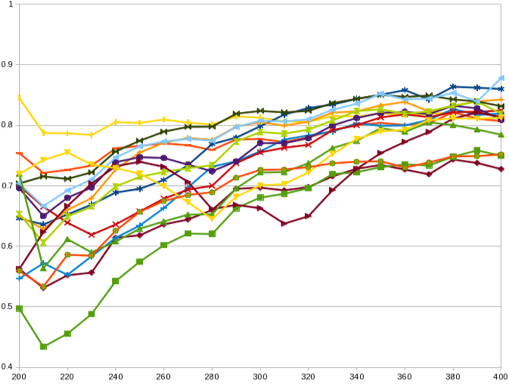
\includegraphics[width=0.99\columnwidth, height=0.7\columnwidth]{img/mirrorsReflectivityBefore.png}
	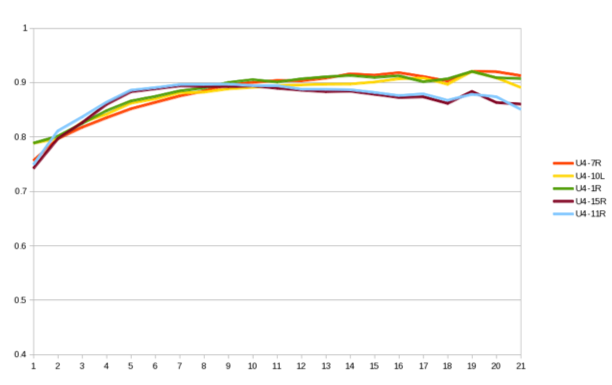
\includegraphics[width=0.99\columnwidth, height=0.7\columnwidth]{img/mirrorsReflectivityAfter.png}
	\caption{Top: Reflectivity measurement as a a function of wavelength of a sample of 8 mirrors before re-coating,
            each sampled at two different places on their surface. The reflectivity
			was measured using a monochromator (Newport model CS260-USB-1-FH-A) with a deuterium light source with a reach
            between 200 nm and 400 nm. The average reflectivity was about 65$\%$ instead of an optimal 90$\%$.
			Bottom: Reflectivity measurement as a function of wavelength of a sample of 5 mirrors measured
            after gluing on the Lexan strips (see text for detail).
            Note the very high value of reflectivity in the UV region, where most of the Cherenkov light is produced.
            In the visible spectrum, the reflectivity is about 90$\%$.}
	\label{fig:reflectivityBeforeAndAfter}
\end{figure}


\subsubsection{Re-coating of cylindrical mirrors}

The cylindrical mirrors range from 6 to 12 inches in length. Each mirror is made from a single piece of aluminum or plastic.
Due to their small size, they fit in most vacuum chambers used to coat mirrors by evaporation of aluminum with magnesium fluoride
(AlMgF$_2$). After successful testing of re-coating of AlMgF$_2$ onto the existing substrate, the work of re-coating the 216 cylindrical mirrors
was awarded to ECI~\cite{ECI}. See \F{reflectivityBeforeAndAfter} (bottom) for typical reflectivity values after re-coating.

\subsubsection{Re-coating of elliptical and hyperbolic mirrors}

The elliptical and hyperbolic mirrors are composed of a Kevlar support structure with a Lexan substrate.
It was not possible to changed this hardware from its original design and construction in 1997.
The support material, which allowed for pitch, roll, and yaw alignment of the mirrors, included
wood and aluminum that was glued to the support structure.

Several companies attempted to re-coat these mirrors but failed due to the outgassing of the various materials.
Furthermore, many of the mirrors are $>$1 m in length, longer than most vacuum chambers.
Therefore the AlMgF$_2$ could not be re-deposited directly onto the mirror substrates.

A different approach consisted of coating thin (25 $\mu$m) Lexan strips and gluing the strips onto the mirror substrate.
While promising, this presented the challenge of protecting the coated Lexan strip from shipping and handling and
from the gluing procedure to the mirrors.

A working chain was setup to:

\begin{enumerate}
	\item coat the Lexan strip
	\item protect the strip with a temporary peel-able film for shipping and handling
	\item ship to Jefferson Lab
	\item glue the strip to mirror substrates
	\item remove the protective film
	\item test the reflectivity
\end{enumerate}

An example of unwrapping the film off the Lexan strip is shown in \F{filmOnStrip}. Several companies produced various test samples with
various protective material films. The job was eventually awarded to ECI \cite{ECI}.
The gluing of the strips to the mirror was done at Jefferson Lab. The mirrors were vacuum-holded on a supporting structure.
Loctite spray contact adhesive glue was applied on the mirror and directed out by a venting system.
The strip was applied to the substrate and after 24 hours of curing time the film was removed.
The typical reflectivity of the refurbished mirrors is shown in \F{reflectivityBeforeAndAfter} (bottom).


\begin{figure}
\centering
	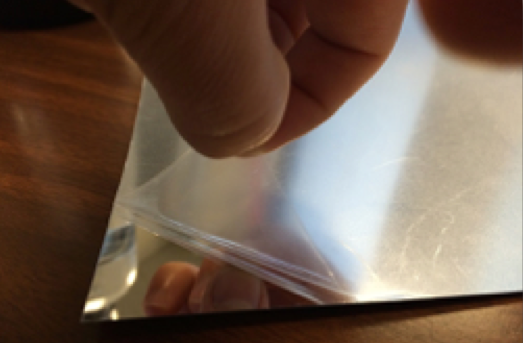
\includegraphics[width=0.98\columnwidth, height=0.7\columnwidth]{img/filmOnStrip.png}
%	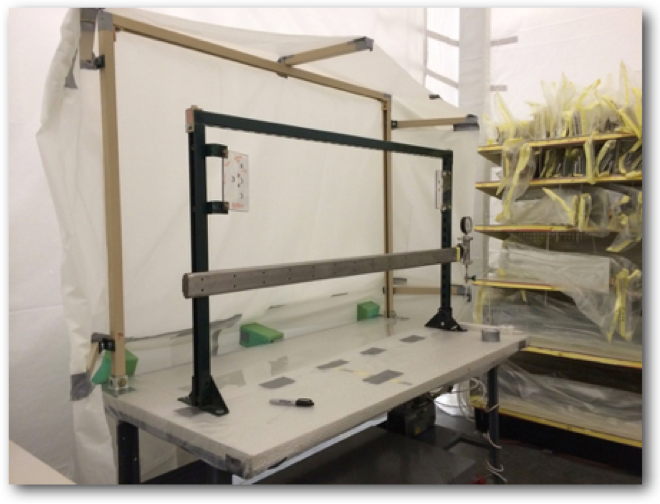
\includegraphics[width=0.98\columnwidth,keepaspectratio]{img/mirrorSetup.png}
	\caption{The protective film. For the elliptical and hyperbolic mirrors the Lexan strips were coated with AlMgF$_2$
			 and covered with films to protect the mirrors during handling and the gluing on top of the mirror substrates.
             The photograph shows the process of removing the protecting film from one such strip.
             The surface reflectivity was tested immediately after the installation on the substrate and again 48 hours after that.
             Only the samples from ECI \cite{ECI} resulted in a consistent high reflectivity. }
	\label{fig:filmOnStrip}
\end{figure}


\subsubsection{Elliptical mirror gaps}

The LTCC elliptical mirrors, especilly the longest ones, presented several gaps between the mirrors, some a few cm long.
This was evident also in the data analyses as a loss of efficiency between the mirrors.
To make sure that no light is lost in these gaps, additional 120 $\mu$m thick Lexan extension strips were produced and coated with AlMgF$_2$.
These strips were manufactured by ECI~\cite{ECI}. They were fitted and glued on left side elliptical mirrors to cover the gaps,
see \F{gapBeforeAndAfter}.

\begin{figure}
\centering
	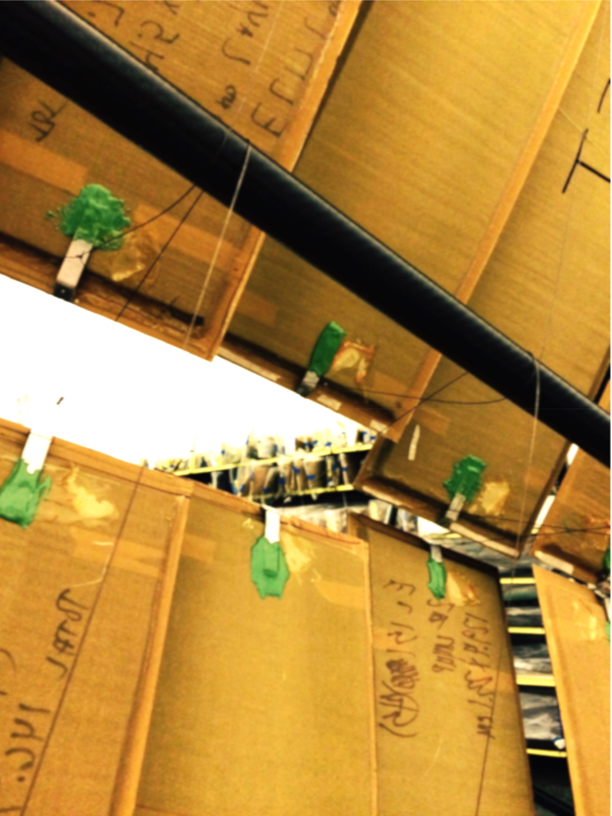
\includegraphics[width=0.98\columnwidth, height=0.7\columnwidth]{img/gapBefore.png}
	\includegraphics[width=0.98\columnwidth, height=0.7\columnwidth]{img/gapAfter.png}
	\caption{Top: the gaps between mirrors before refurbishing LTCC. These gaps were also seeing in the data as
			 drop of efficiency near the middle of the detector, as the Cherenkov light was not collected.
             Bottom: all the gaps are covered by the extension strips.}
	\label{fig:gapBeforeAndAfter}
\end{figure}


\subsubsection{Mirror re-coating summary and results}

All 216 cylindrical mirrors were re-coated on the existing surface. All 216 elliptical and 216 hyperbolic mirrors were refurbished using Lexan strips
coated with AlMgF$_2$ glued onto the substrate. The different sizes of the mirrors were accounted for using different widths for the Lexan strips, see
summary Table~\ref{tab:strips}.


\begin{table}
	\begin{center}
		\begin{tabular}{| l | c |}
			\hline \hline
			Quantity  & Dimensions (inches) \\
			\hline
			190       & 9  x 36 x 0.010  \\
			150       & 10 x 36 x 0.010  \\
			6         & 10 x 36 x 0.010  \\
			\hline \hline
		\end{tabular}
	\end{center}
	\caption{Summary of material used for the elliptical and hyperbolic mirrors. The total length of the Lexan strip necessary to re-coat the 216 elliptical
            and 216 hyperbolic mirror was 310 meters.}\label{tab:strips}
\end{table}


In \F{reflectivityBeforeAndAfter} (bottom) a typical spectrum of reflectivity that applies to all cylindrical, elliptical, and hyperbolic mirrors is shown.
The re-coated mirrors show a $\sim 90\%$ reflectivity in the visible spectrum and an exceptional $\sim 80\%$
reflectivity in the UV spectrum.



\subsection{Mirror alignment}

A new procedure was developed to align the mirrors within the LTCC boxes that takes advantage of their focusing capabilities.
The elliptical mirror focal points (see \F{alignmentSimulation}) are 1. the target (origin of the lab coordinate system)
and 2. a point behind the hyperbolic mirror. The focal points of the hyperbolic mirrors are 1. a point near the focal point of the elliptical mirrors and
2. a point above the face of the PMTs.

The geometrical shape of the mirrors has been built into the CLAS12 Geant4 simulation \cite{gemc2019}.
When a laser line coming from the target is directed at the mirror,
it is focused on the hyperbolic focal point, then directed at the PMT, see \F{alignmentSimulation}.
This geometrical focusing was used during the mirror alignment: a 3 mW, 635 nm laser was placed, relative to the detector,
in center of the CLAS12 coordinate system, the location of the liquid-hydrogen target and the first ellipse focal point.
The laser was mounted on a structure that allowed the beam direction and line angle to move with respect to the floor, while keeping
the origin of the laser at the coordinate system origin.
This position was accurate at the 0.5 mm level. The laser was spread through two cylindrical lenses into a laser line and shone
longitudinally along the center-line of each elliptical mirror. Both the elliptical and hyperbolic mirrors were then
adjusted in pitch, roll, and yaw to minimize the light spot dimensions and to center it in the middle of the face of the PMT.
The PMT entry glasses were protected from the laser line with custom-fitted cardboard pieces. After alignment, the spot size of the laser was 5 mm.


\begin{figure}
\centering
	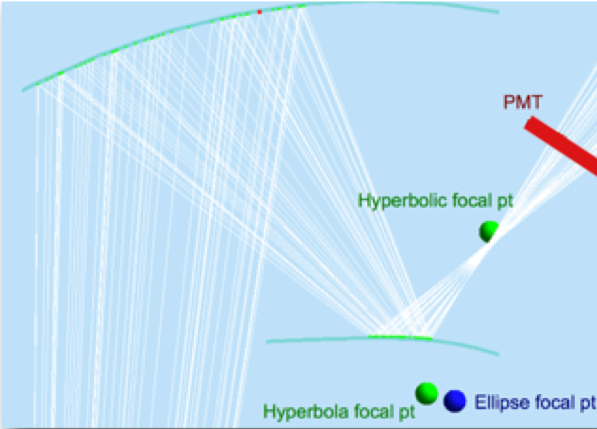
\includegraphics[width=0.99\columnwidth,  height=0.75\columnwidth]{img/mirrorAlignmentSimulationZoomed.png}
	\caption{The simulation of a laser line (white tracks are photons) originating from the target (first ellipse focal point) and directed at the elliptical mirrors.
             The photons are reflected to the second ellipse focal point. The hyperbole first focal point is near the ellipse focal point so the hyperbolic mirror
			 reflects the incoming photons to the hyperbole second focal point, located above the face of the PMTs.
			 This picture illustrates the procedure used for the alignment: the mirror positions are adjusted until the laser line originating from
			 the target is focused on the face of the PMT.}
	\label{fig:alignmentSimulation}
\end{figure}


%\begin{figure}
%\centering
%	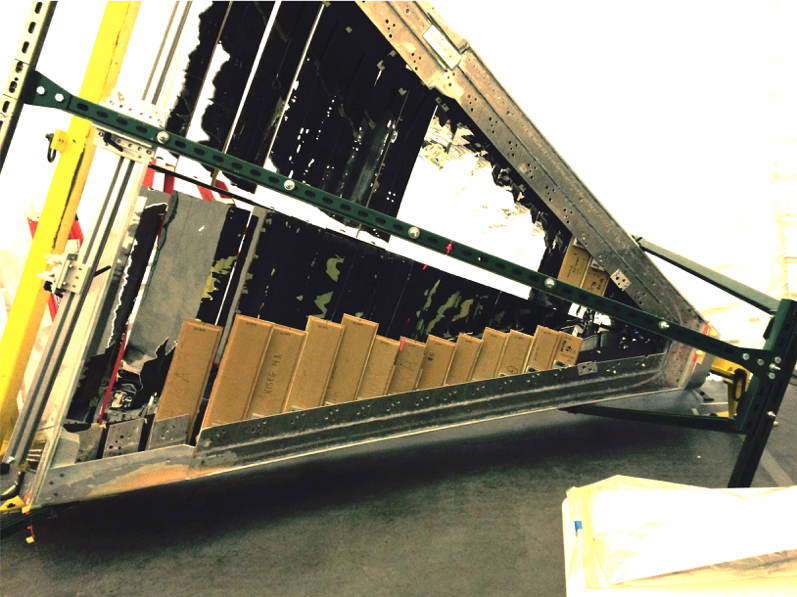
\includegraphics[width=0.95\columnwidth, keepaspectratio]{img/laserAlignment1.png}
%	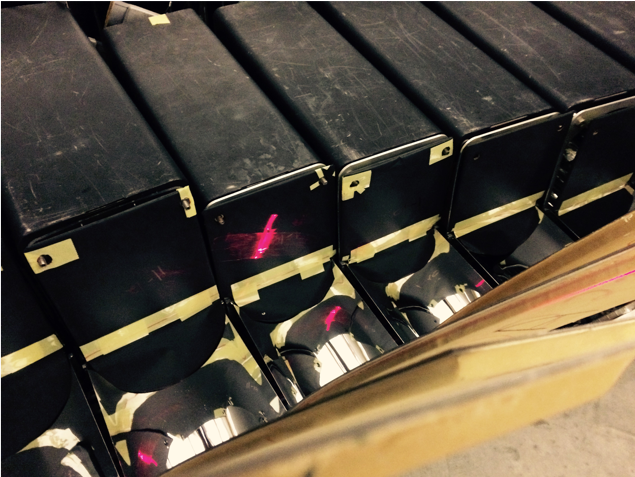
\includegraphics[width=0.95\columnwidth, keepaspectratio]{img/laserAlignment2.png}
%	\caption{The laser alignment setup. Top: the laser was placed, relative to the detector, in the lab coordinate system. The laser line was shined on each elliptical mirror.
%         Bottom: zoomed in view of the laser line focused on the center of the PMT after the mirrors were aligned.}
%	\label{fig:laserAlignment}
%\end{figure}


\subsection{Photo-multipliers surface coating}

The PMTs used in the LTCC are the photonis are the Photonis XP4500B \cite{Photonis:2007ta}.
Their borosilicate windows can be used to detect wavelengths as low as approximately
$300$ nm. However the Cherenkov light is inversely proportional to the wavelegth, see eq.~\ref{eq:cerenkov},
the $C_4F_{10}$ gas is transparent down to wavelengths of $180$ nm, and the mirrors and WCs reflectivities is non zero
even for wavelengths below $200$ nm: the limiting factor of enhanced QE in the UV region
is the transparency of the window material of the PMTs. UV-glass windows can detect photons down to
250 nm, and only quartz windows can efficiently detect light down to 180 nm. While quartz windows maximize the UV-sensitivity
of the PMT, and therefore the Cerenkov detector performance, they are difficult and expensive to produce.

A wavelength shifter (WLS) deposited on the face of a borosilicate or UV glass
PMT provides an effective alternative to boost the efficiency of a \u{C}erenkov
detector by converting UV photons with a wavelength below $300$ nm into two
isotropically emitted photons with longer wavelengths.



\begin{figure}
	\centering
	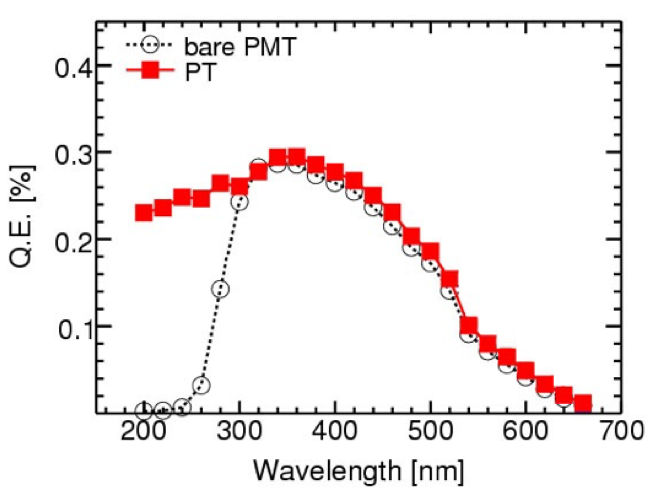
\includegraphics[width=1.0\columnwidth,keepaspectratio]{img/pmtQuantumEfficiencyGain.png}
	\caption{Average number of reflections calculated from simulations studies.}
	\label{fig:pmtQuantumEfficiencyGain}
\end{figure}

\begin{figure}
	\centering
	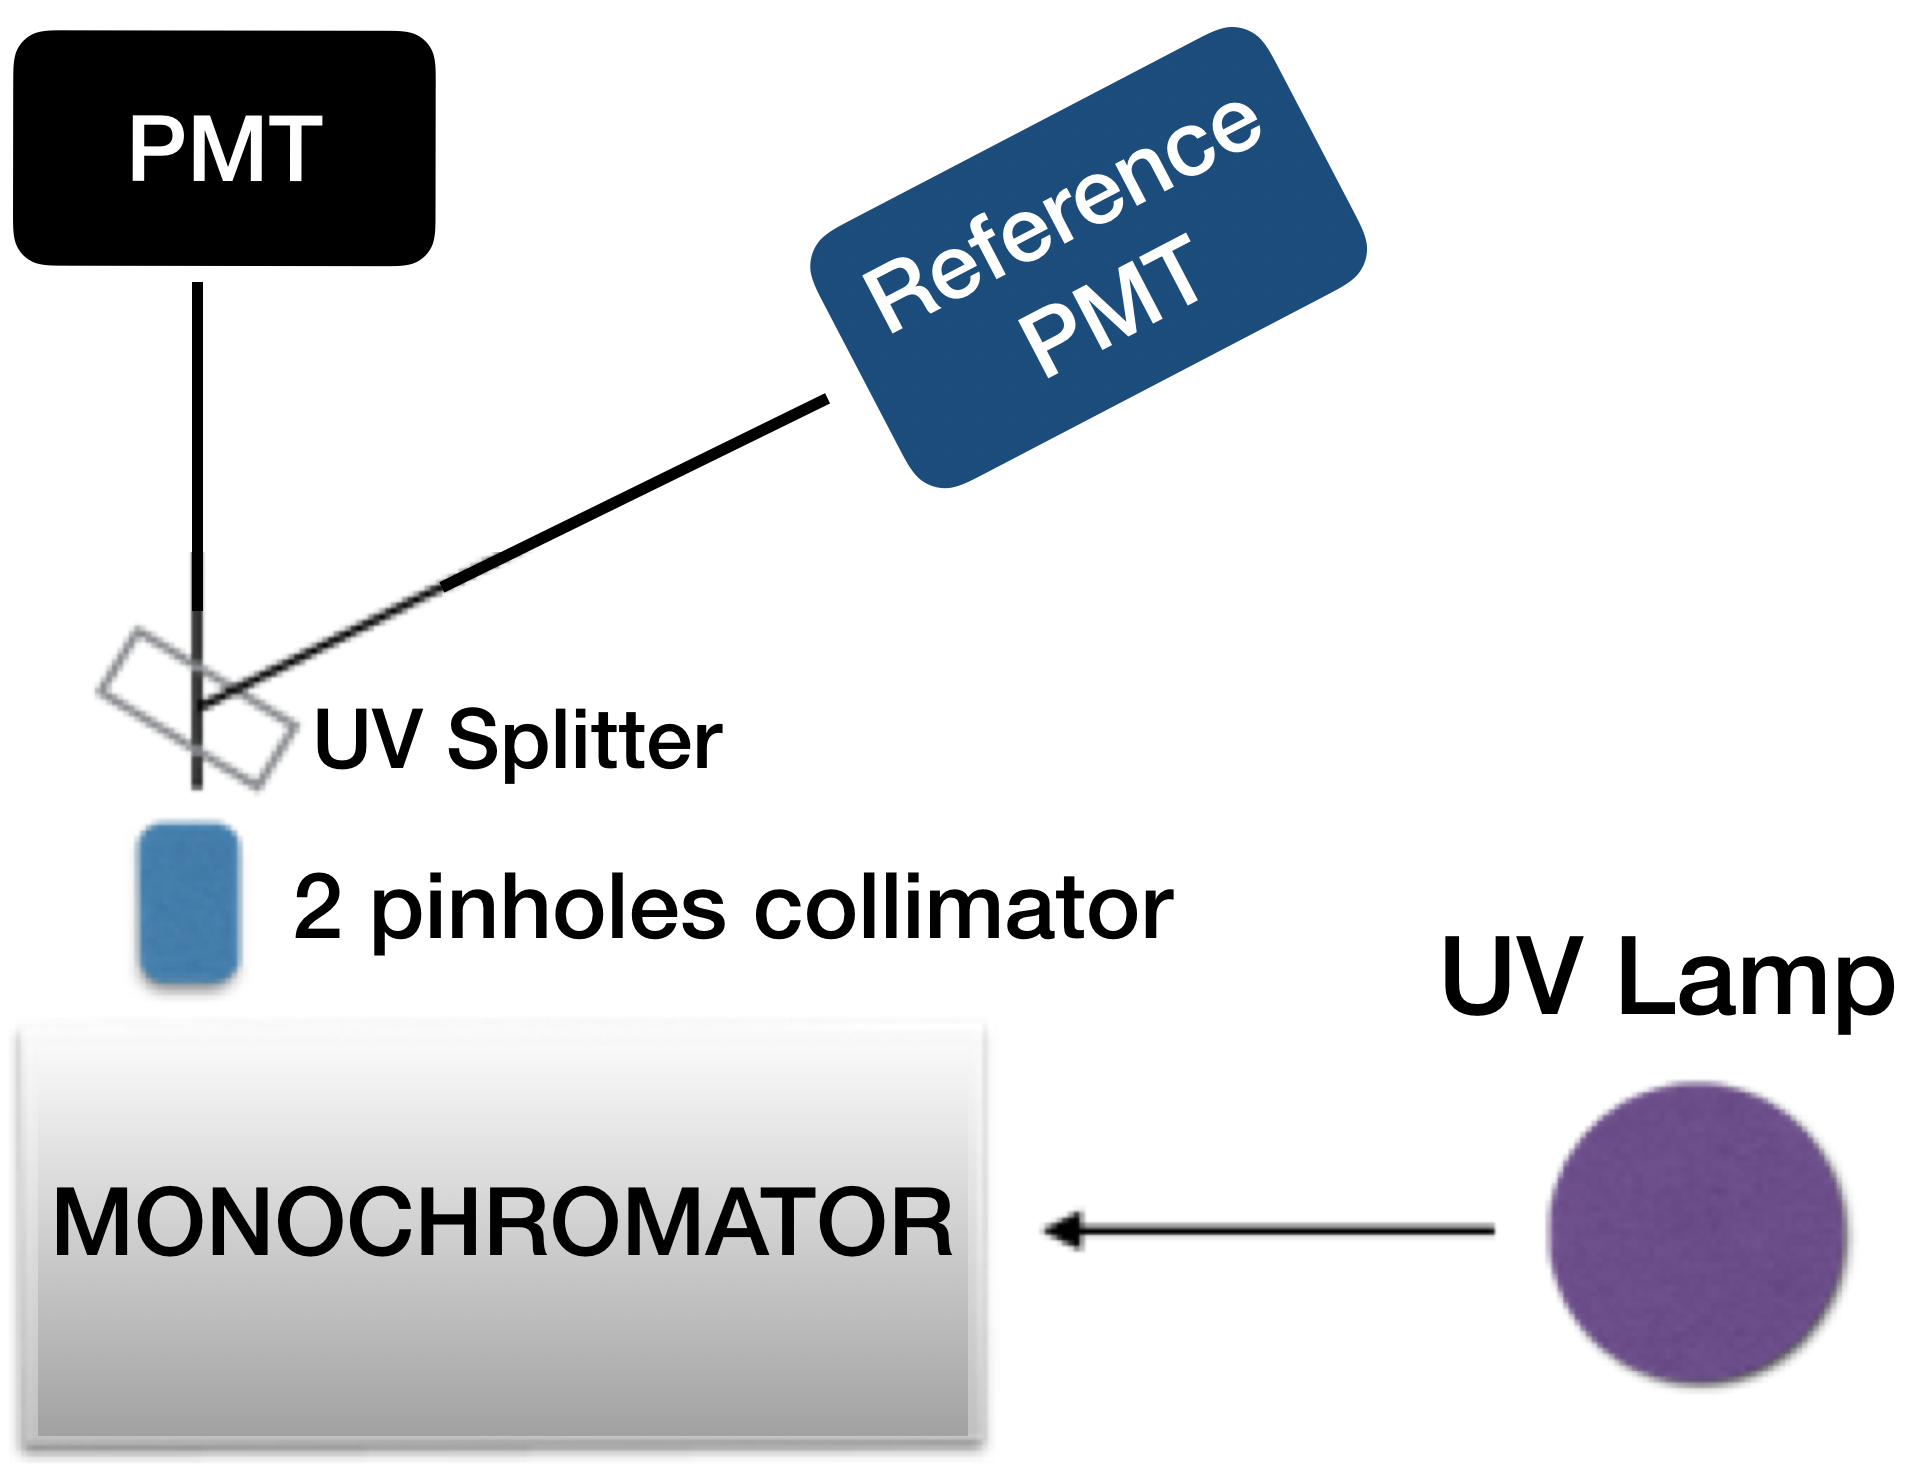
\includegraphics[width=1.0\columnwidth,keepaspectratio]{img/pmtTestingSetup.png}
	\caption{Average number of reflections calculated from simulations studies.}
	\label{fig:pmtTestingSetup}
\end{figure}




\subsection{Winston cone refurbishment}

Winston cones (WC) are used to collect light onto the PMTs. In the LTCC there are three kind of WCs:

\begin{enumerate}

\item Small
	\begin{enumerate}
		\item Height: 18 cm
		\item Radius at the top: 20 cm
		\item Radius at the bottom: 11 cm
		\item Material: 0.25 cm thick copper (electro-formed)
	\end{enumerate}

	\item Medium
	\begin{enumerate}
		\item Height: 22 cm
		\item Radius at the top: 20 cm
		\item Radius at the bottom: 11 cm
		\item Material: 0.5 cm thick plastic (vacuum pressed)
	\end{enumerate}

	\item Large
	\begin{enumerate}
		\item Height: 30 cm
		\item Radius at the top: 22 cm
		\item Radius at the bottom: 11 cm
		\item Material: 0.25 cm thick copper (electro-formed)
	\end{enumerate}
\end{enumerate}

\begin{figure}
	\centering
	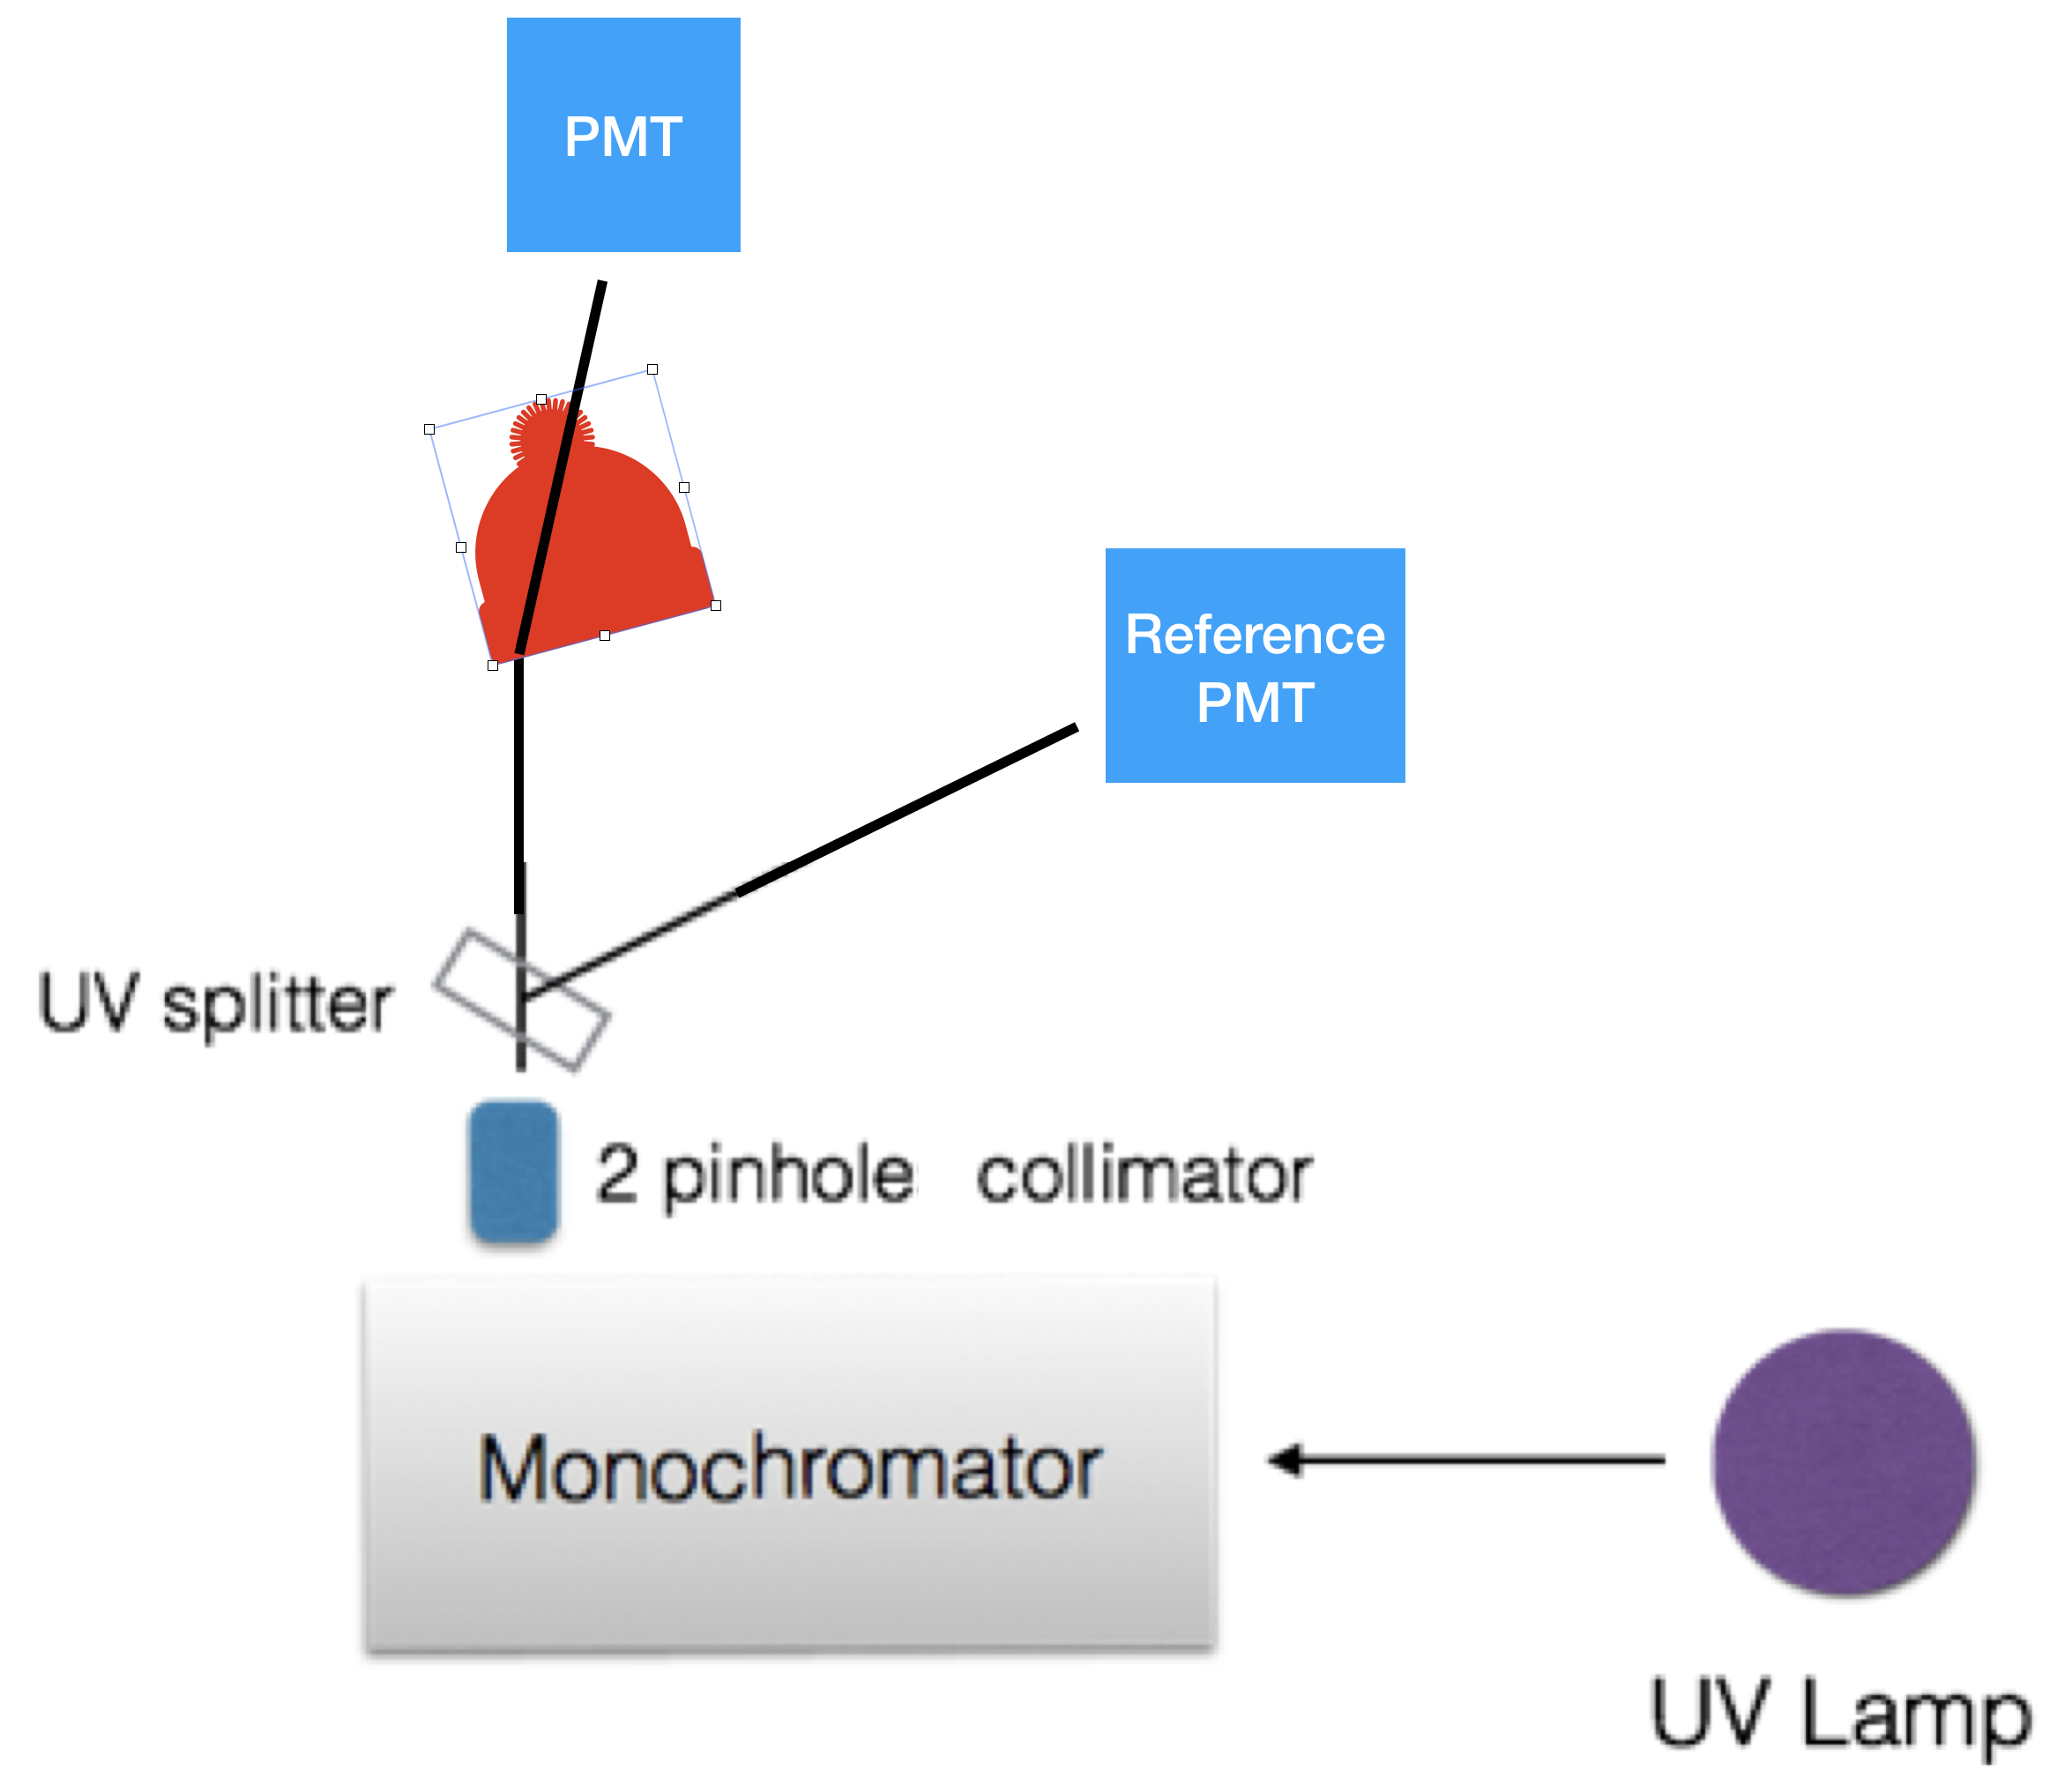
\includegraphics[width=0.95\columnwidth,keepaspectratio]{img/wcSetup.png}
	\caption{Setup to measure the WC reflectivity. The wavelength of light from a deuterium lamp was measured using a mono-chromator and splitted in two
            light beams, each with calibrated intensity. One of the light beam impinged on the WC at a typical angle of 12 degrees,
            while the other was directed at the reference PMT. }
	\label{fig:wcSetup}
\end{figure}

The reflectivity of the WC showed the same degradation as the mirrors. However, due to their shape, re-coating of the WC is more costly than the mirrors and the budget allowed
refurbishing of only 160 out of 216 total WCs.
A setup on an optical bench to measure the reflectivity for all the cones at wavelengths between 200 and 400 nm was designed to accept incident
shallow angles of 10-15 degrees (typical incidence angle based on simulation studies), see \F{wcSetup}. A typical reflectivity of a poor WC is shown in \F{wcStatusBefore} (top).
All 216 WC were measured, and the results are shown in \F{wcStatusBefore} (top). This allowed cataloging ofthe quality of the WC to select the worst ones to refurbish,
see \F{wcStatusBefore} (bottom).
The cones were put in a vacuum chamber and $AlMgF_2$ was deposited on top of the existing coating. The typical reflectivity of WC after recoating is shown in \F{wcStatusAfter} (top).
About 30 cones needed the additional treatment of removing the existing aluminum coating to improve the new $AlMgF_2$ deposition. Even then, about half of these cones did not show improvements.
The results of the WCs refurbishment are summarized in \F{wcStatusAfter} (bottom).


\begin{figure}
	\centering
	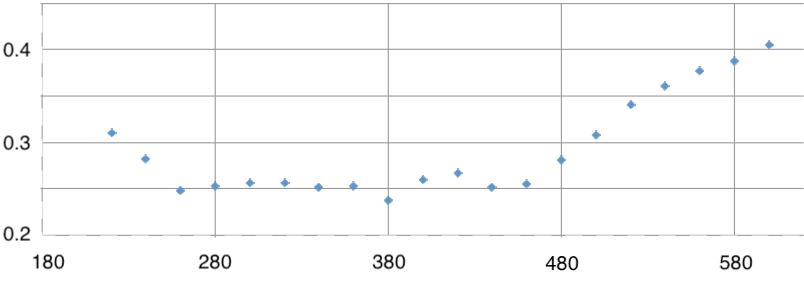
\includegraphics[width=0.95\columnwidth,keepaspectratio]{img/winstoConeSample2Reflectivity.png}
	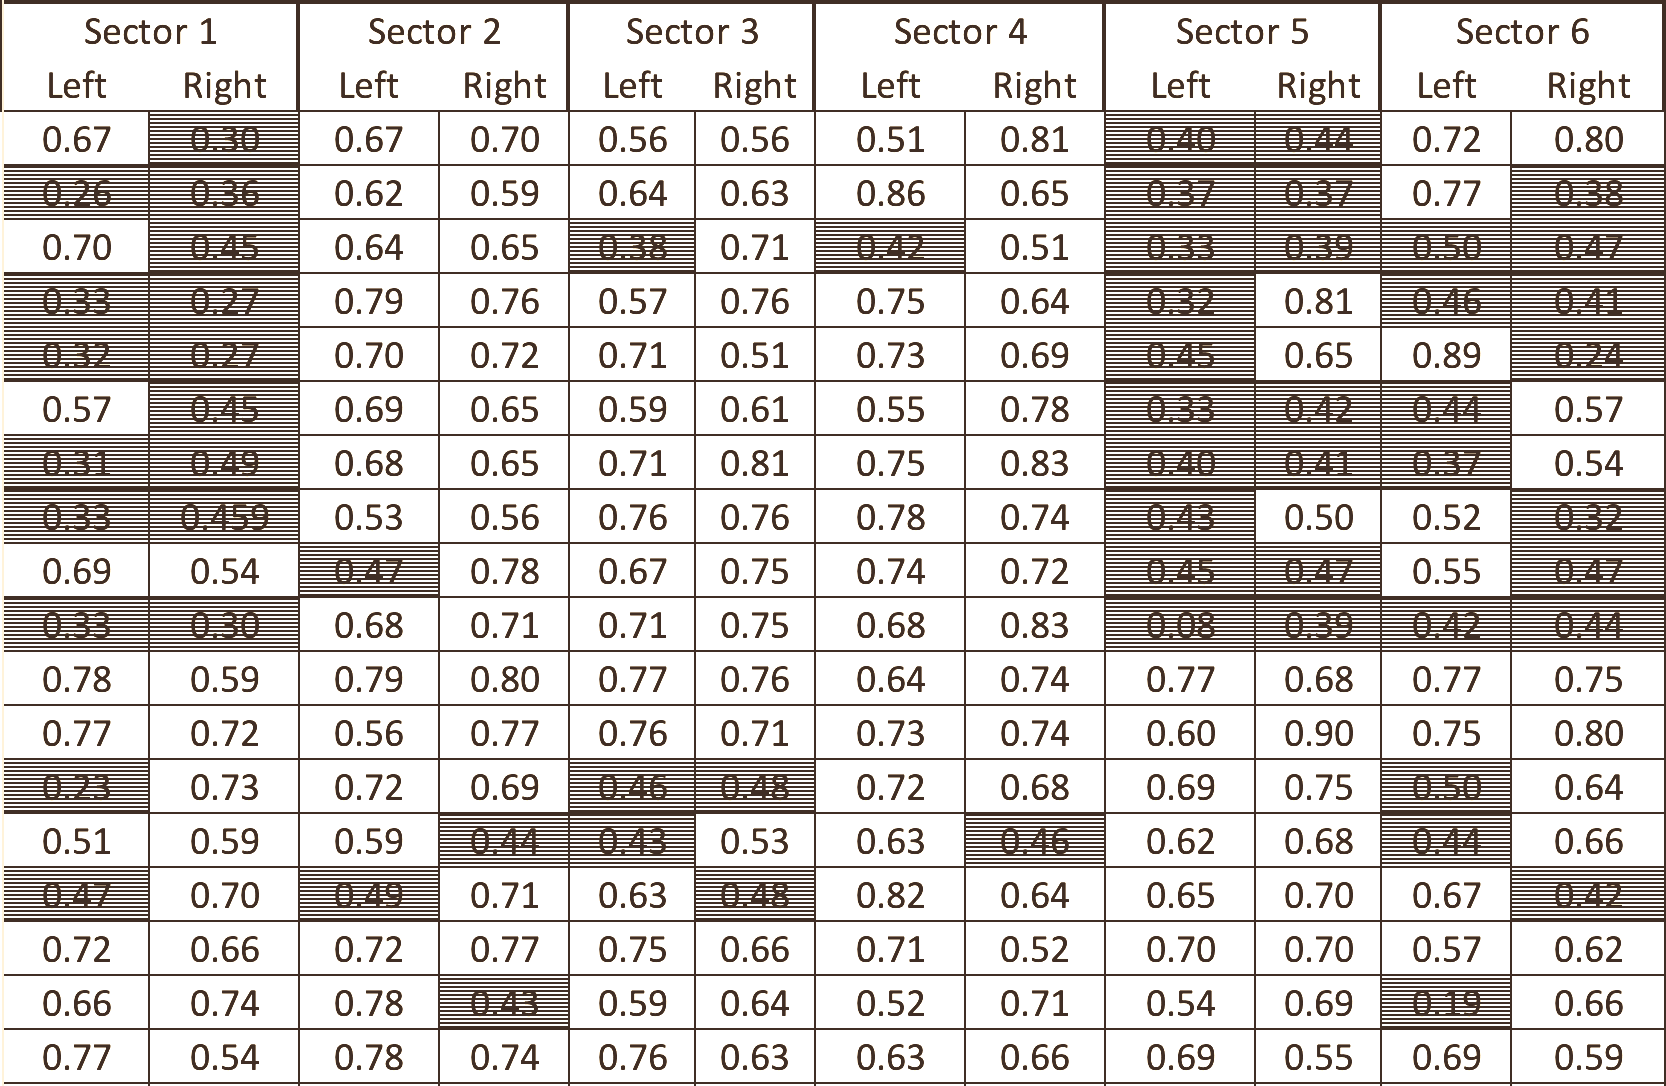
\includegraphics[width=0.95\columnwidth,keepaspectratio]{img/wcStatusBefore.png}
	\caption{Top: typical reflectivity of a "very poor" WC. The reflectivity is below 30\% for most of the wavelength between 200 and 400 nm. Bottom: the average reflectivity $r$ between 200 and 400 nm for
            all the WC. Legend: grey: ``very poor'' ($r < 30\%$); red: ``poor`` (30\% < $r < 50\%$); brown: ``so-so`` (50\% < $r < 70\%$); green: ``good`` (70\% < $r < 80\%$); yellow: ``excellent`` ( $r > 70\%$); }
	\label{fig:wcStatusBefore}
\end{figure}


\begin{figure}
	\centering
	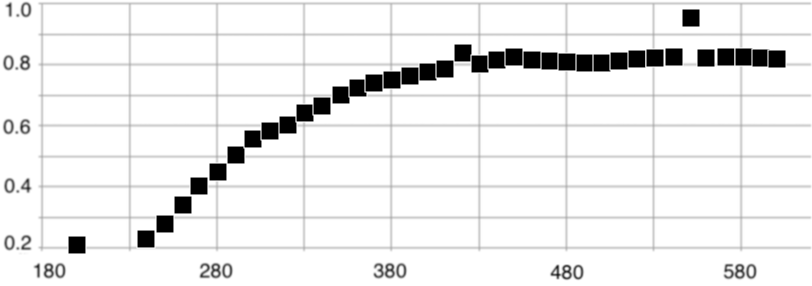
\includegraphics[width=1.0\columnwidth,keepaspectratio]{img/winstoConeSample1Reflectivity.png}
	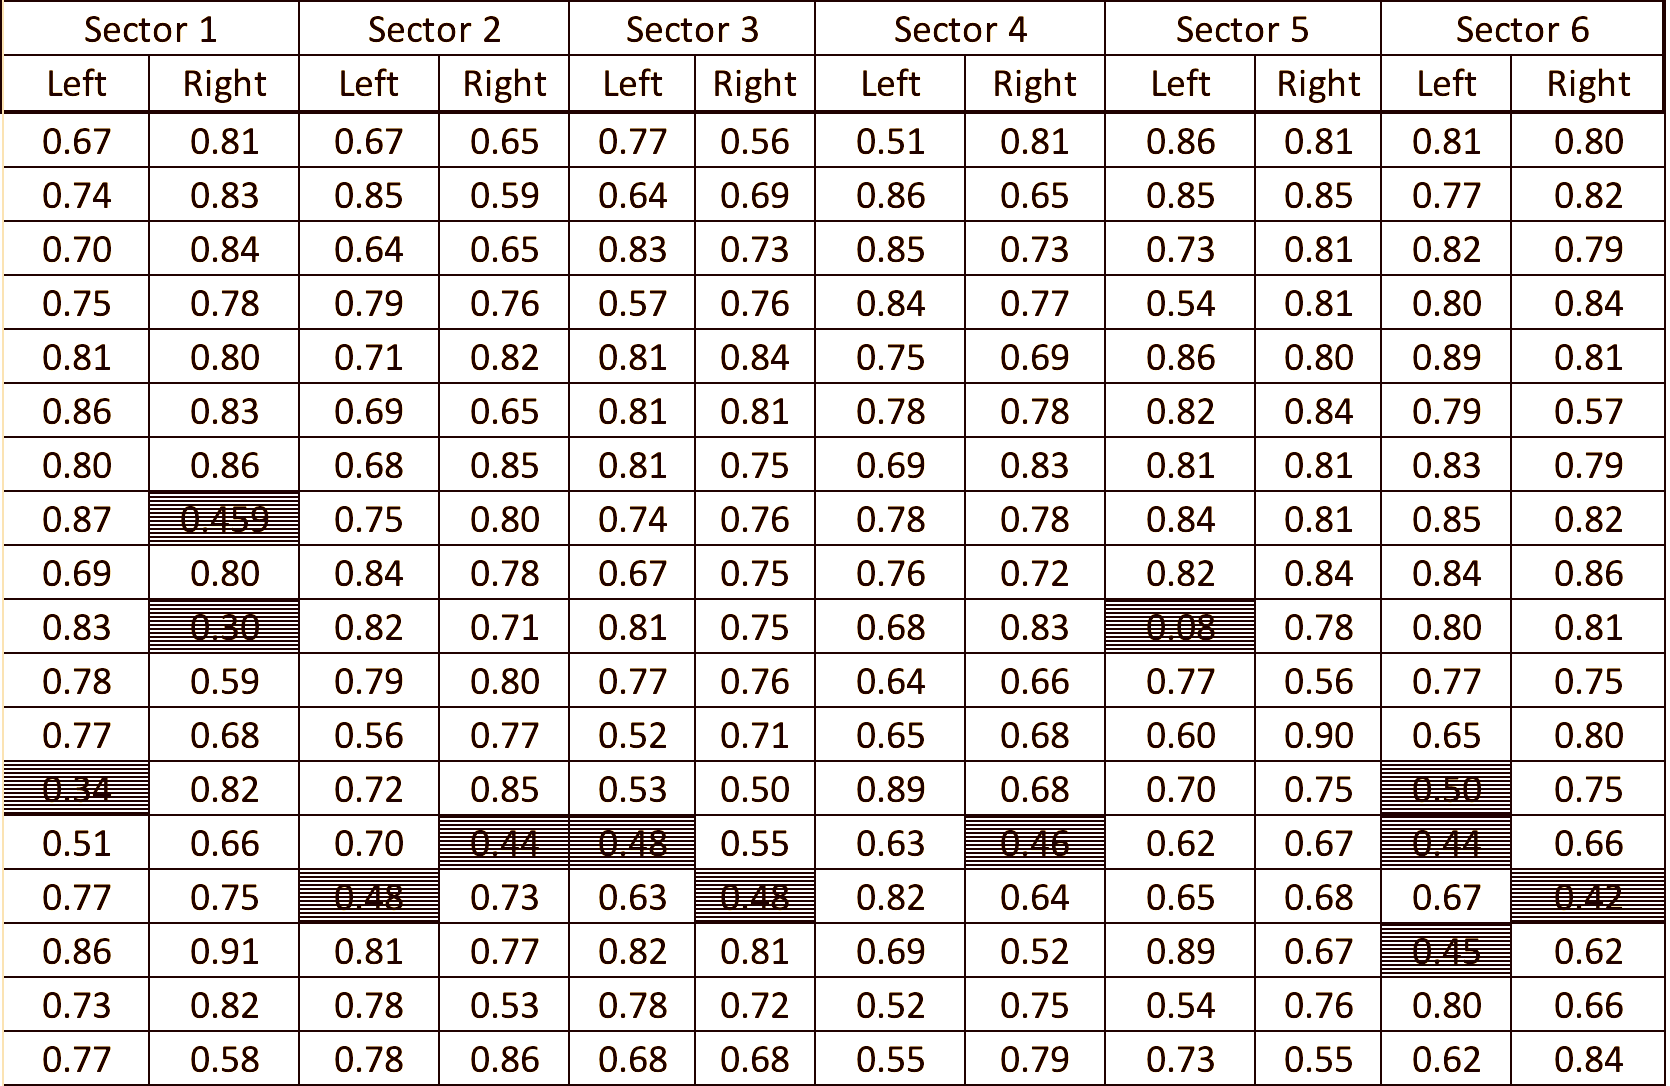
\includegraphics[width=1.0\columnwidth,keepaspectratio]{img/wcStatusAfter.png}
	\caption{Top: typical reflectivity of a "very poor" WC after refurbishment. The reflectivity quickly rise to $to\%$ at a wavelength of about 340 nm. Bottom: average WC reflectivity  $r$ between 200 and 400 nm for
				all the WC. This picture should be compared to \F{wcStatusAfter}. }
	\label{fig:wcStatusAfter}
\end{figure}



\subsection{The LTCC Windows}

The LTCC windows that cover the upstream and downstream open frame of the box are a composite of
Tedlar/Mylar/Tedlar, see \F{windowDesign}. Two layers of the Tedlar film provide reliable light tightness
even if they have some defects such as wrinkles and small pinholes through, while the Mylar portion
adds the material strength necessary to withstand gas differential pressure and increase wear resistance
and reliability. This design, easy to handle and apply to the module,
simplified the replacement of the old composite window.

\begin{figure}[!ht]
	\centering
	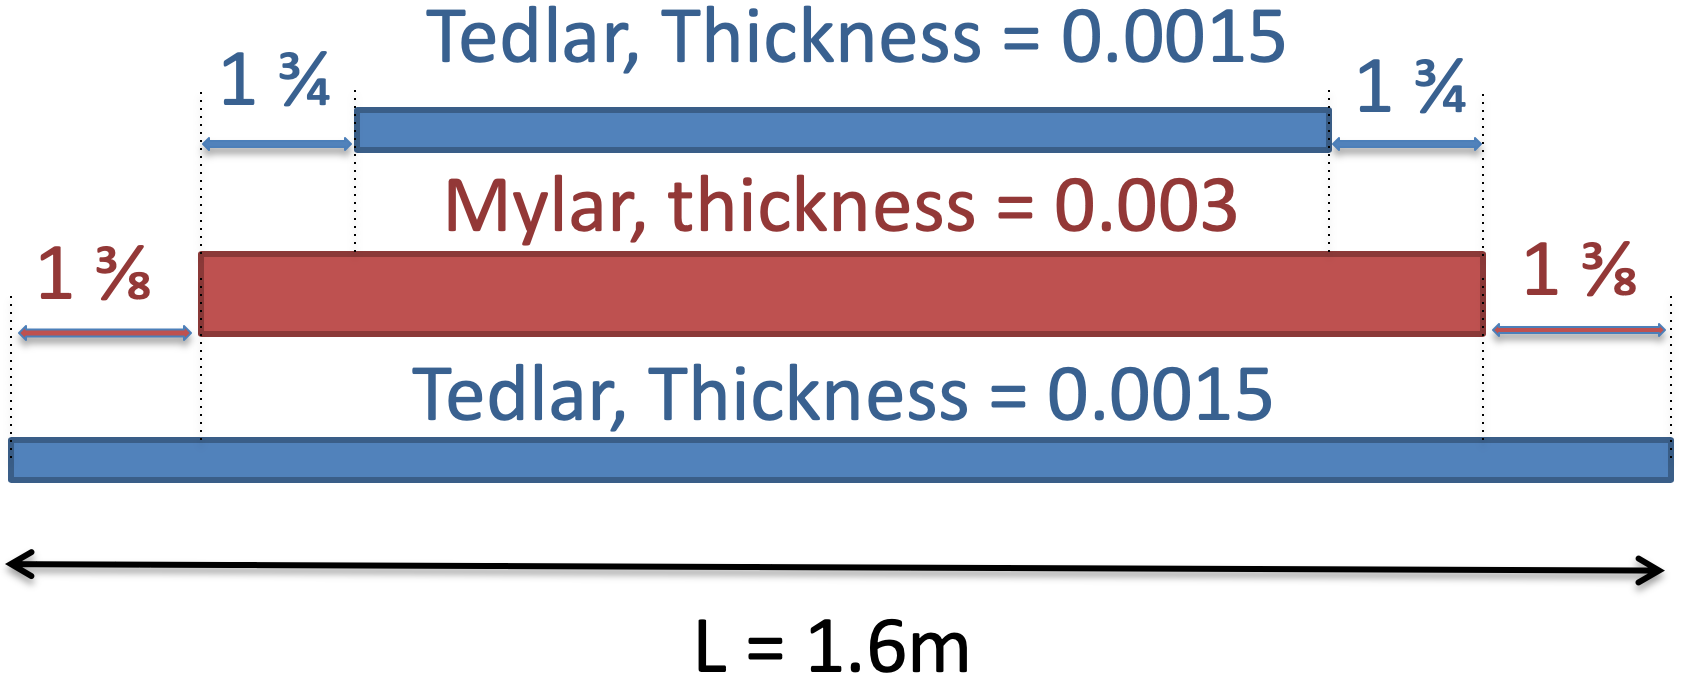
\includegraphics[width=0.98\columnwidth, keepaspectratio]{img/windowDesign.png}
	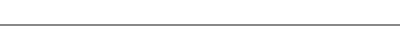
\includegraphics[width=0.98\columnwidth, height=0.1\columnwidth]{img/blank.png}
	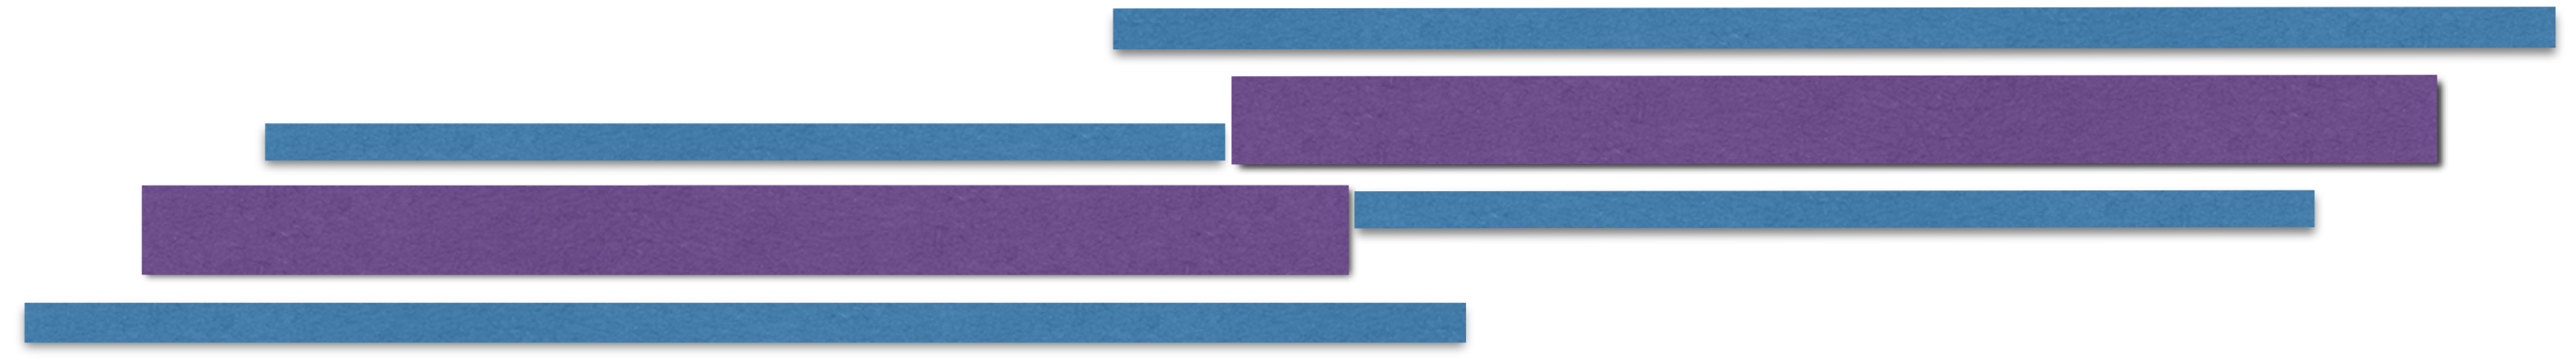
\includegraphics[width=0.98\columnwidth, keepaspectratio]{img/windowSeaming.png}
	\caption{Top: the design of the LTCC Tedlar/Mylar/Tedlar window sandwich. The pyramid design allowed for the
          seaming shown at the bottom. Bottom: the seaming design involves gluing Mylar to Mylar to ensure that the window
          stress is transmitted entirely to the Mylar.}
	\label{fig:windowDesign}
\end{figure}


The window was fabricated in two steps:

\begin{enumerate}
	\item lamination of 1.6~m wide Tedlar/Mylar/Tedlar rolls
	\item seaming of the laminated strips into a 4.8~m $\times$ 4.8~m window
\end{enumerate}

The lamination of the composite material, with dimensions outlined in \F{windowDesign} (top), was performed at
Madico~\cite{madico}, where a sheet 400~m long was produced.

At Jefferson Lab rectangles were cut out of the laminated sheet, each 1.6~m wide and 4.8~m long. To form a final
4.8~m $\times$ 4.8~m single LTCC window, three of the rectangles were seamed together using G/Flex 655 epoxy.
The seam was load tested to withstand a pressure 10 times higher than that expected from the C$_4$F$_{10}$ gas flow and gas weight.

\subsubsection{Window Installation and Gas Leak Tests}

The installation of the window onto the box was achieved through gluing the window on the box sides using G/Flex 655
epoxy. The width of the window attached with glue was 12~cm, to provide sufficient gluing area. A photograph of the
downstream window after installation is shown in \F{downstreamWindow}.

\begin{figure}
	\centering
	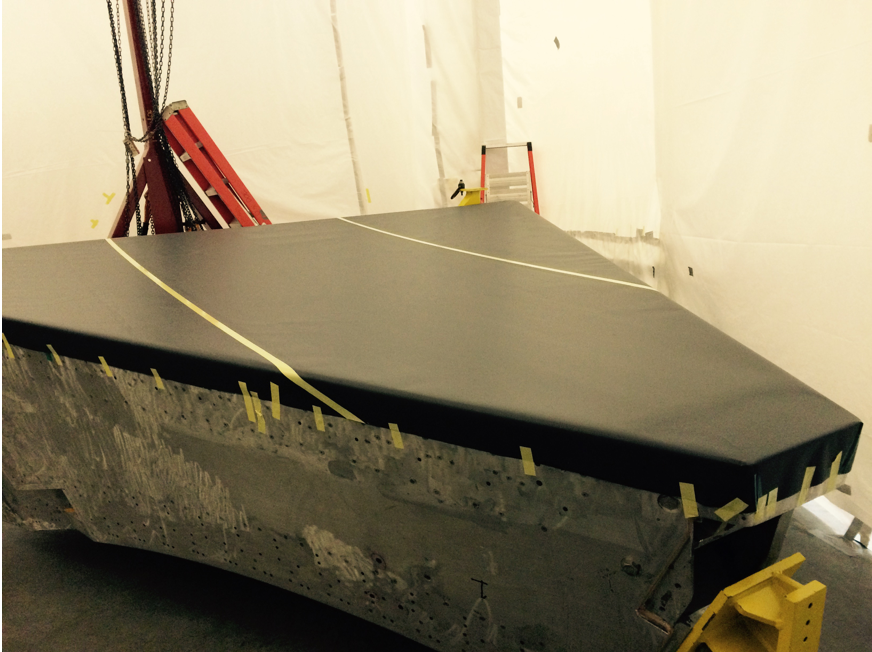
\includegraphics[width=1.0\columnwidth,keepaspectratio]{img/downstreamWindow.png}
	\caption{The downstream window of one LTCC sector during curing of the epoxy. The yellow strips protect the
          window seaming.}
	\label{fig:downstreamWindow}
\end{figure}

After curing of both the upstream and downstream windows, the LTCC box was filled with nitrogen gas to a
positive differential pressure of
2~in of water. Freon gas was pumped into the box and leaks were detected using a refrigerant leak detector. After the
leaks were sealed, the box was pressurized for a 48 hour period to test the overall box gas tightness. This procedure
was repeated after every movement of the LTCC boxes, as small shifts of the frame walls had the potential to introduce
additional leaks due to the large surface area of the detector.


\section{Electronics and Readout}

\F{electronicScheme} shows a schematic diagram of the electronics and readout used for the LTCC
detector. Since the magnetic shield case is near the bulb of the photomultiplier tube, and the WC is in direct contact
with the bulb, the electrons in the photomultiplier tube could strike the inner bulb wall if the negative voltage
was applied to the cathode. For this reason the signals are capacitatively coupled to positive HV, with the PMT
cathode at ground potential,
and the XP4500B Photonis PMTs anodes are powered with positive polarity by a CAEN SY4527 high voltage
mainframe outfitted with 1501P boards. There are two anode signals from the PMT output. One of them is
connected directly to flash ADC boards built at Jefferson Lab, the Flash ADC module FADC250~\cite{daq-nim}.
The FADC250 sampling frequency is 250~MHz. The other signal is discriminated by the Jefferson Lab built
discriminator scaler module DSC2~\cite{daq-nim}, and connected to CAEN v1190 TDC modules. The TDCs have a
50~ps/channel timing resolution, and the discriminator threshold was set to 30~mV, corresponding to 15\% of the
SPE amplitude. The LTCC FADC250 and TDC information are read out using the CLAS12 data acquisition (DAQ)
system~\cite{daq-nim}.

\begin{figure}
	\centering
	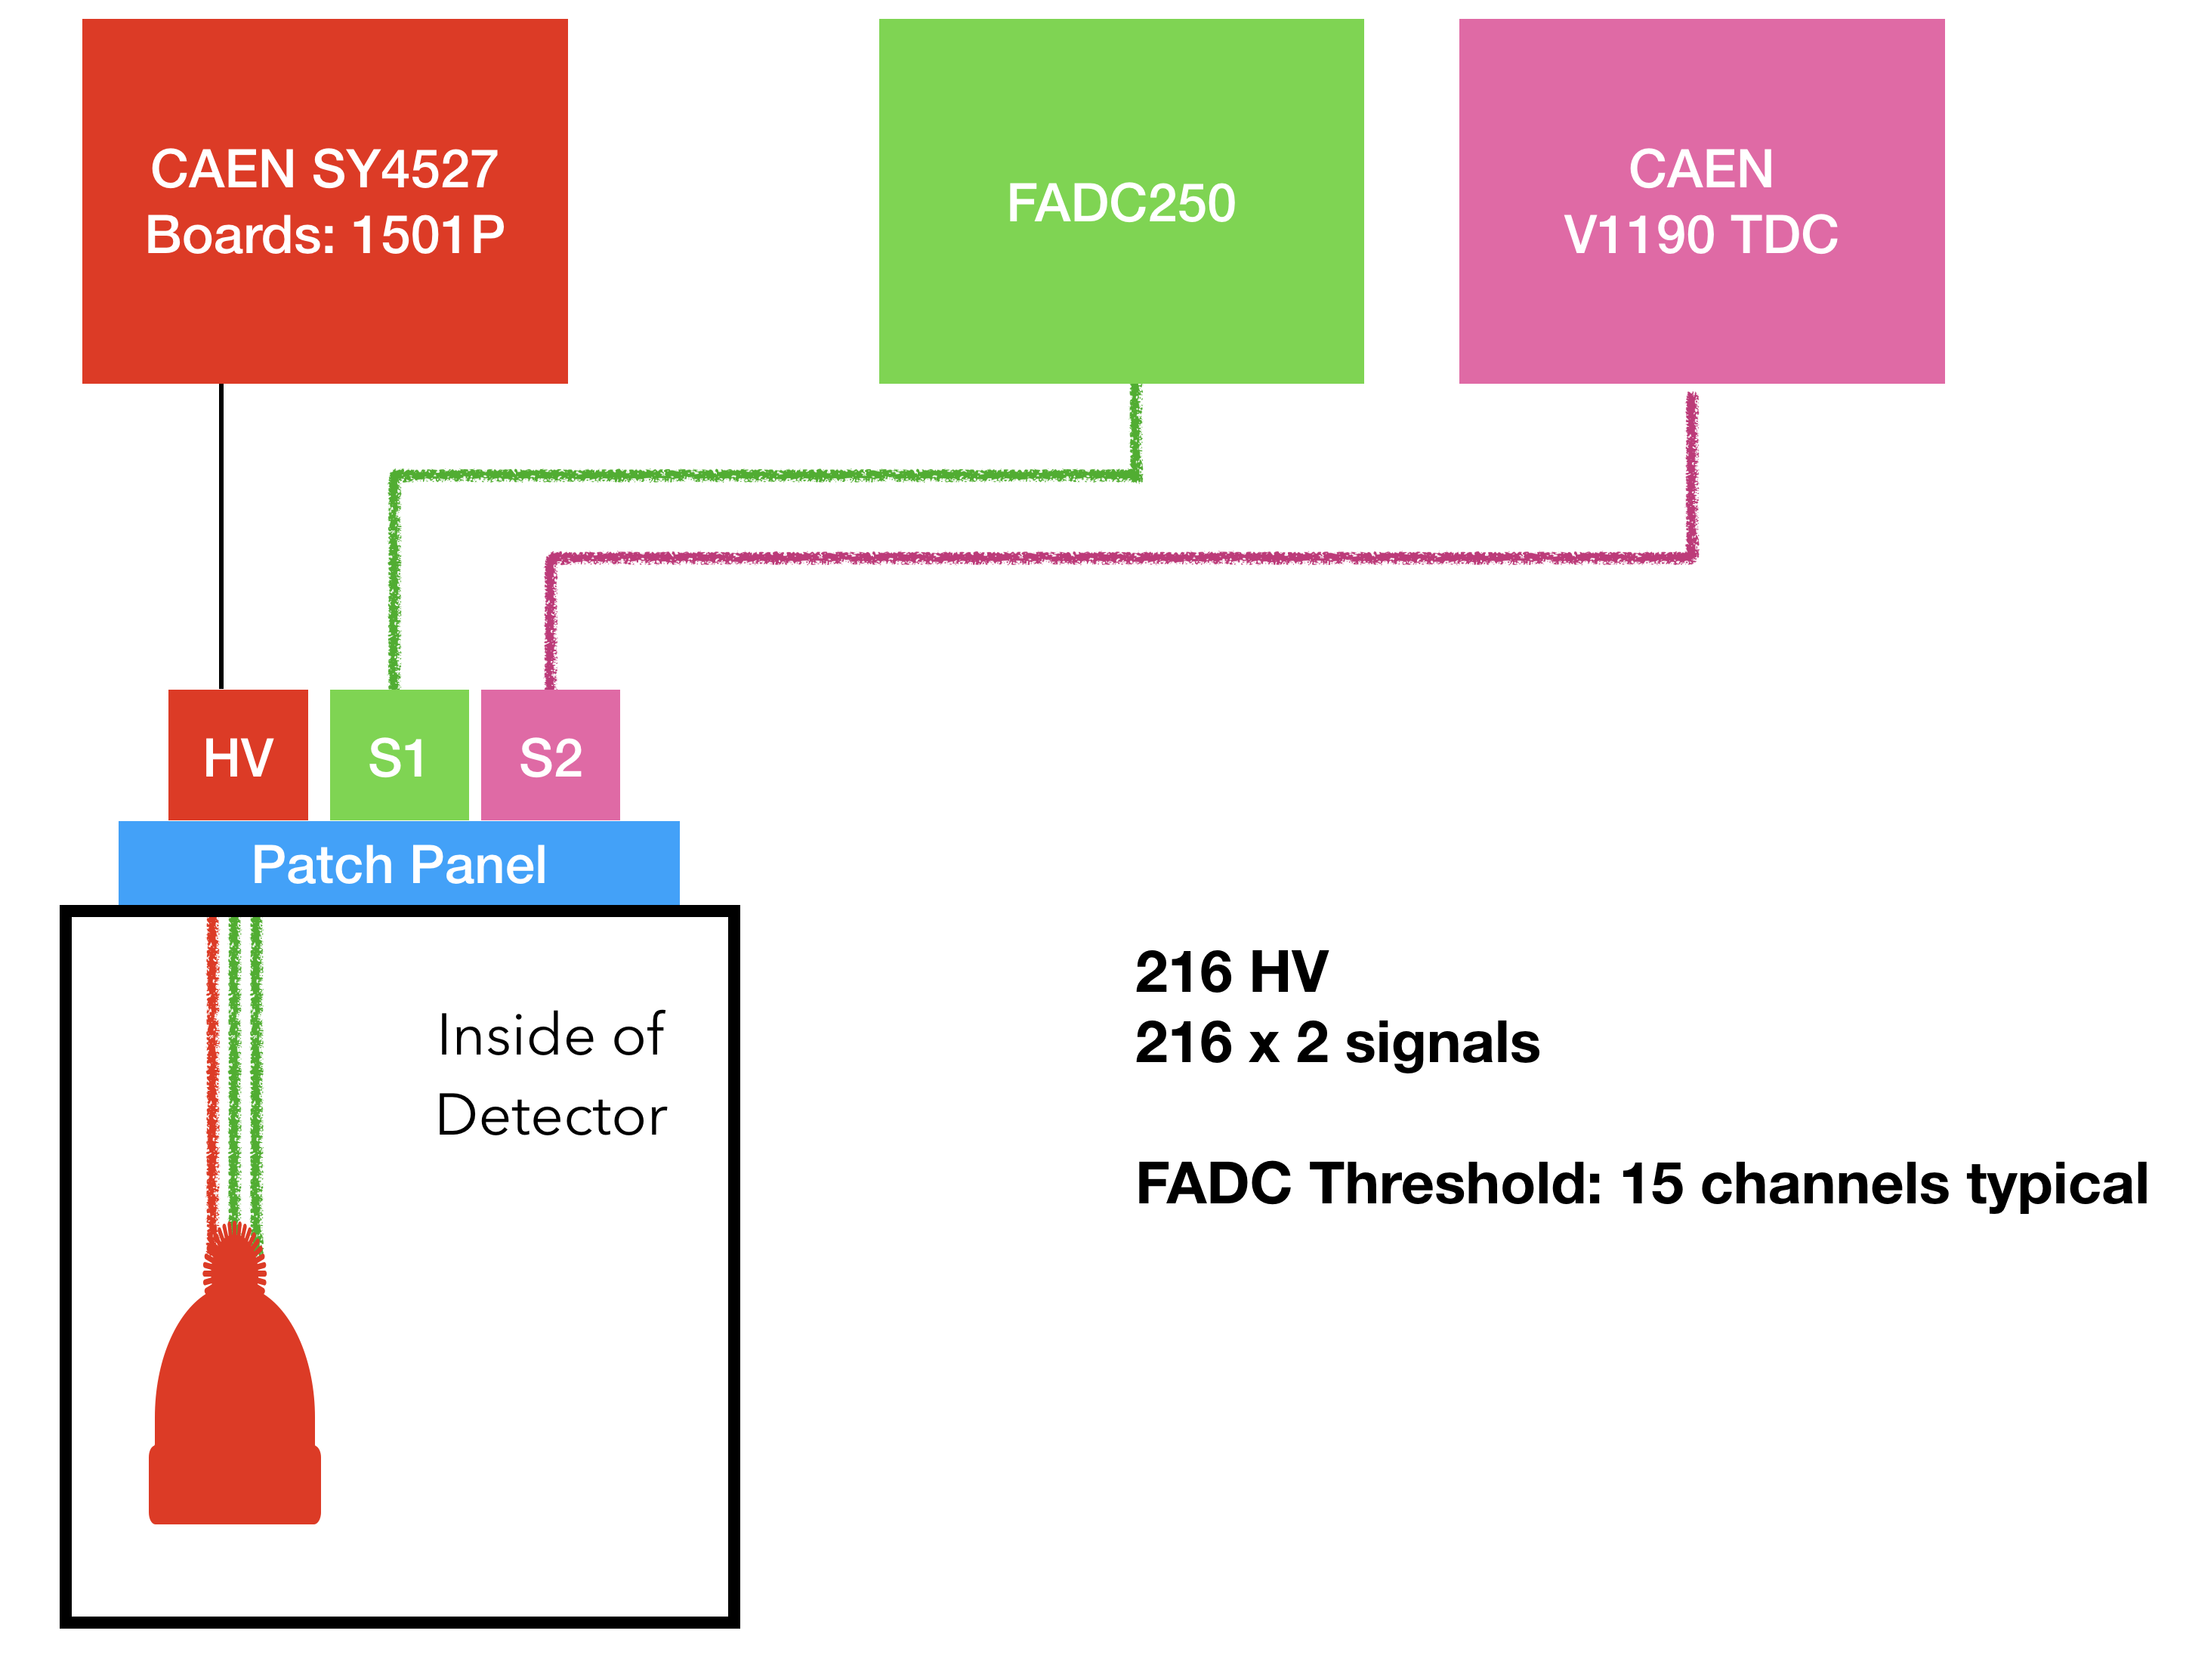
\includegraphics[width=0.99\columnwidth, height=0.6\columnwidth]{img/electronicScheme.png}
	\caption{The electronics schematic of the LTCC. One HV and two readout signals are connected from each PMT
          base to the patch panel. The patch panels then connect the HV to the CAEN SY4527 (1501P boards), one read
          out to the FADC250 and the other to DSC2 discriminators.}
	\label{fig:electronicScheme}
\end{figure}

A typical signal from the FADC250 module is shown in \F{fadc}. The signal is usually contained in 3 to 5 time samples
(each time sample is 4~ns). In order to be written to tape, at least one of the 100 signal samples in the 400~ns
wide readout window must be above a threshold of 30 channels, corresponding to about 30\% of the SPE peak value.
This is well above the typical pedestal variation of 1-5 channels. The FADC250 then integrates the FADC signal over
a time window of 16~ns (4 samples) before the threshold crossing time, for the duration of 20 samples (80~ns). The
final integrated charge used in the reconstruction code is the signal integral minus the electronic pedestal, as
described in \F{fadc}.

\begin{figure}[H]
	\centering
	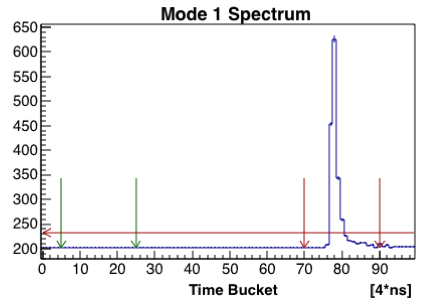
\includegraphics[width=0.99\columnwidth, height=0.6\columnwidth]{img/fadc.png}
	\caption{The FADC250 digitized output as a function of sample index for one of the LTCC PMTs.
          The DAQ system saves a 400~ns time window (100 samples) if at least one of the 100 signal samples is
          above a 30-channel threshold. The integral signal is the sum of the output at the sample indexes between
          the two right arrows, one placed 4 samples before the signal crosses the threshold, and the other placed
          20 samples after that. The final integrated charge used in the reconstruction code is this integral minus
          the pedestal. The pedestal is calculated using the average of the signal between the left arrows. The
          absolute positions of the pedestal acquisition limits and the relative position of the signal integration
          limits are adjusted in the DAQ parameters and loaded before each run.}
	\label{fig:fadc}
\end{figure}

%\begin{figure}
%	\centering
%	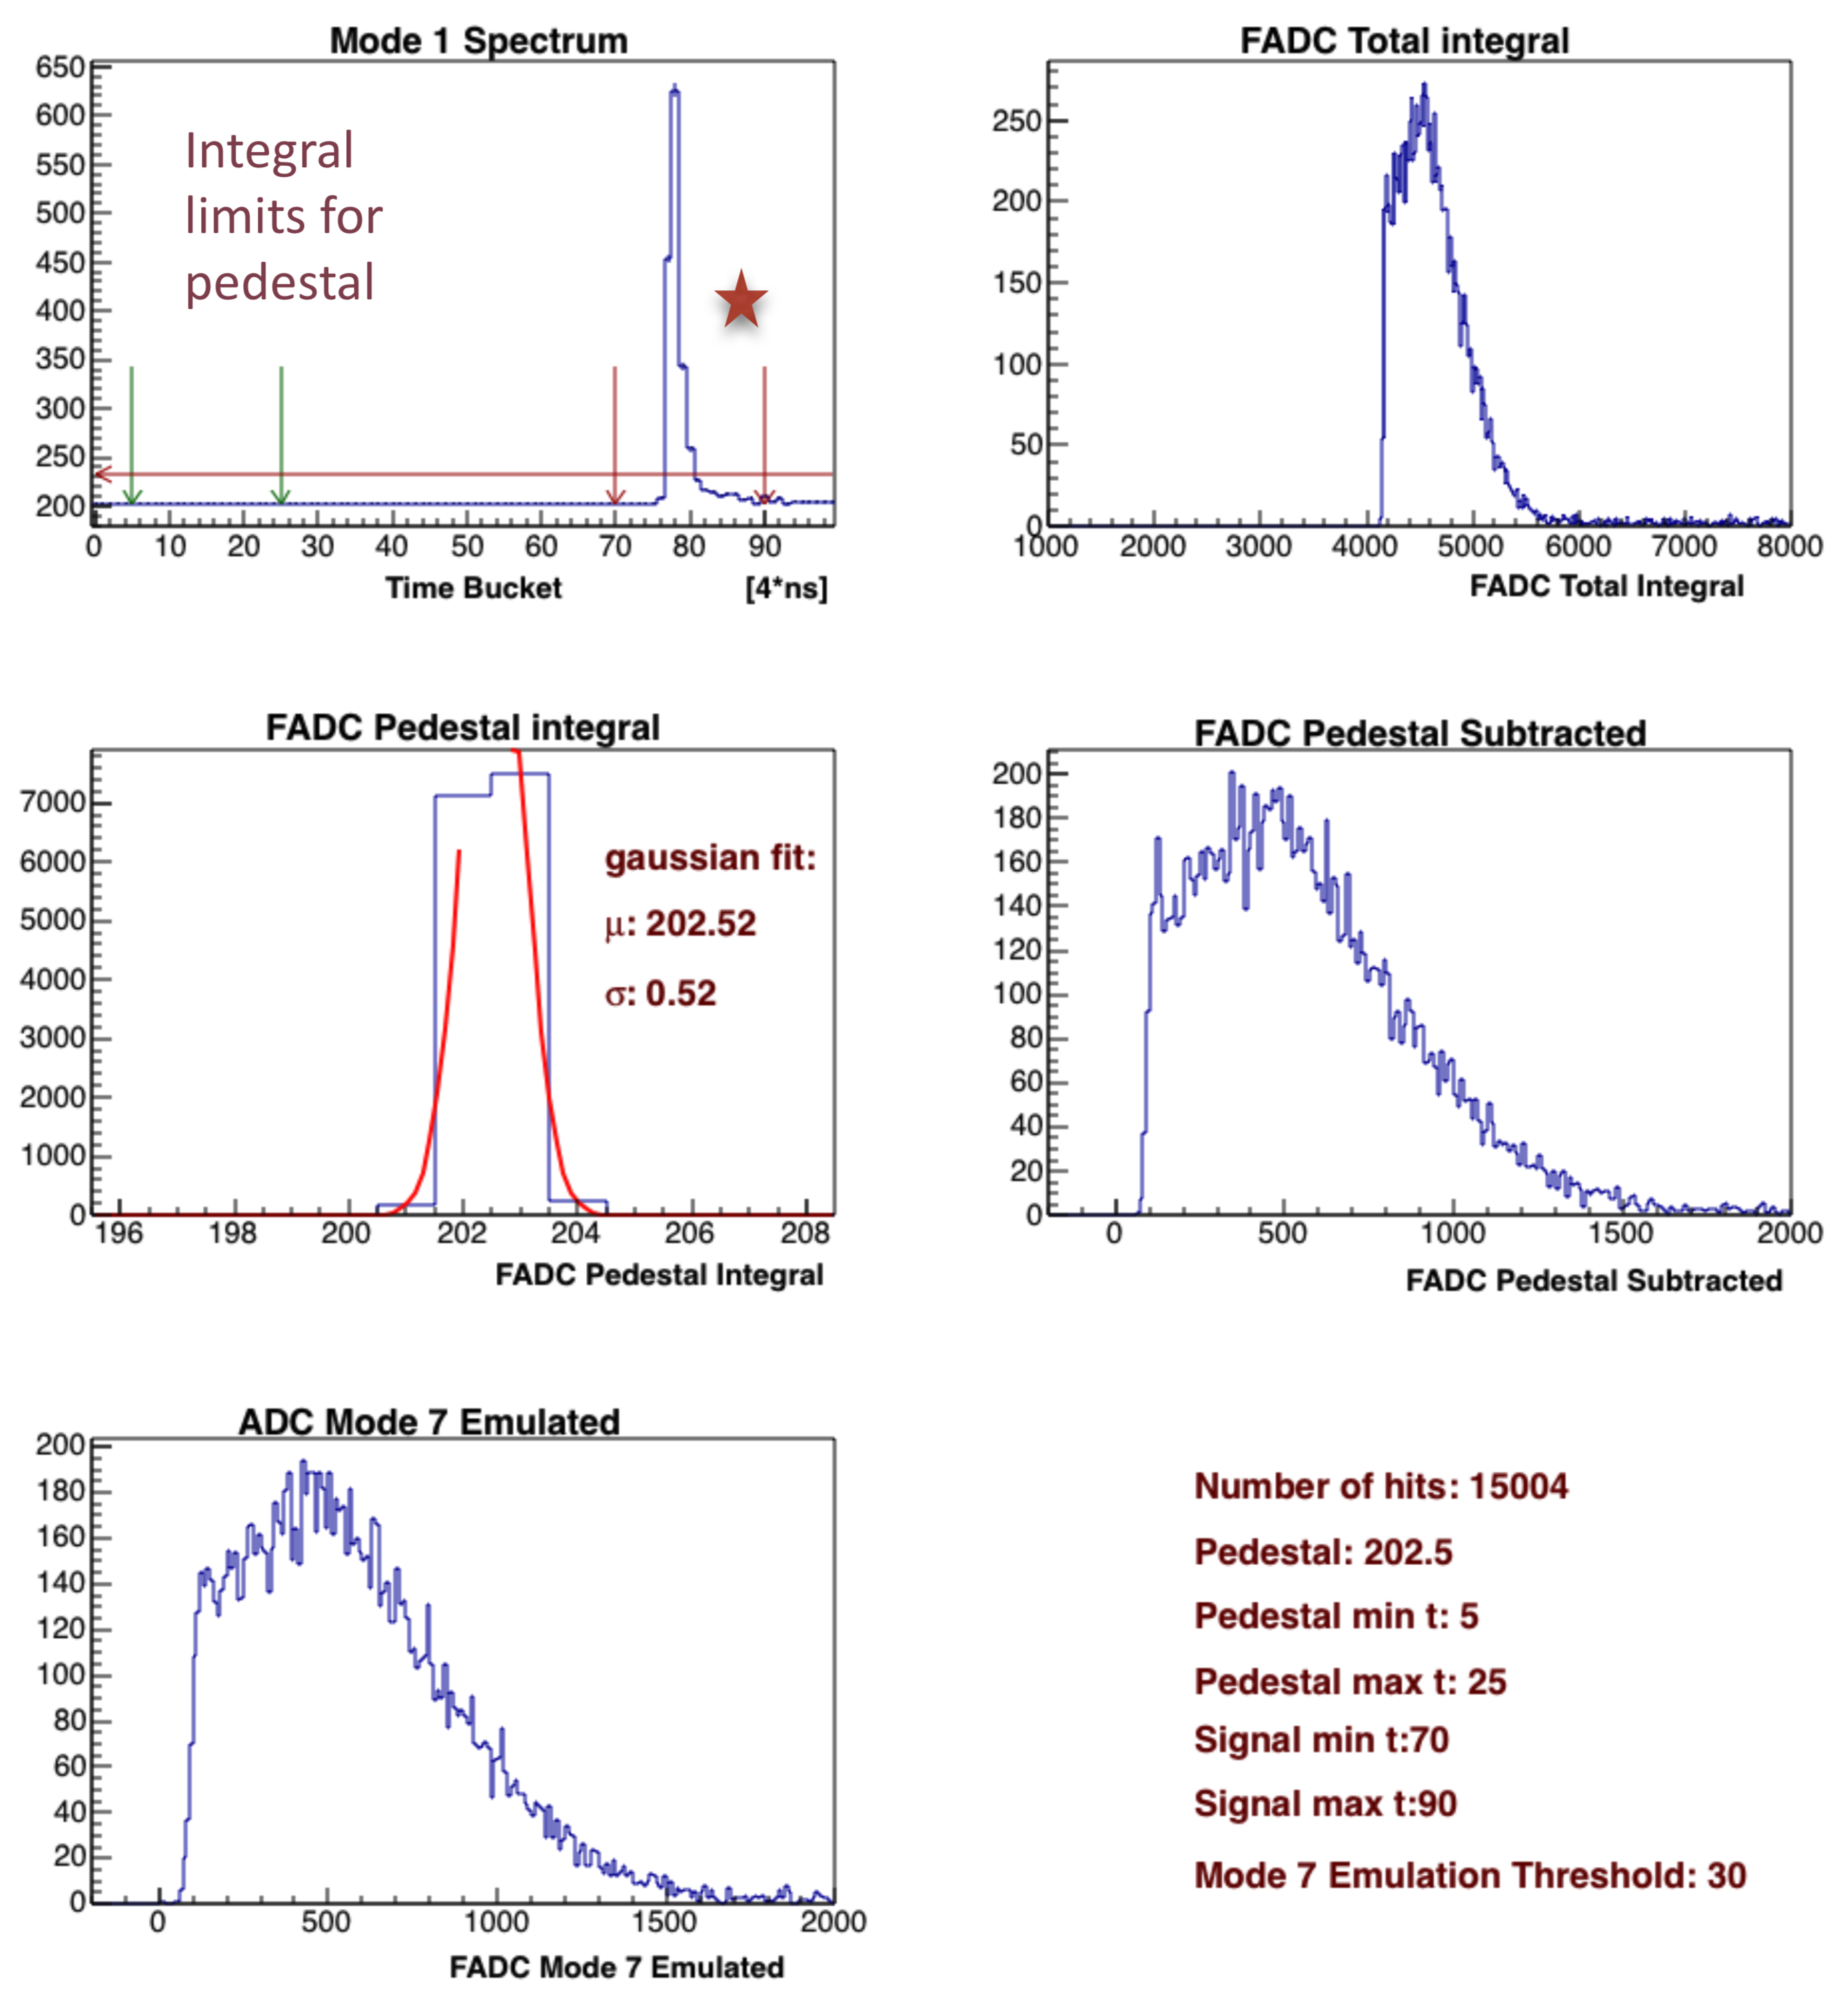
\includegraphics[width=0.99\columnwidth,keepaspectratio]{img/readout.png}
%	\caption{The electronic scheme of the LTCC.}
%	\label{fig:readout}
%\end{figure}

\section{Hardware Components}

New instrumentation modules have been designed by JLab that take advantage of the higher performance and elegant back-plane connectivity of the VITA 41 standard or ``VXS'', defined as VME with serial extensions. 
VXS was selected as the 12~GeV data acquisition back-plane foundation for the front-end detector readout and trigger hardware interface because this standard offered a method to easily synchronize and pass signals between each of the payload slots to a central switch fabric slot. At JLab a dual star back-plane configuration is used, and one switch slot is used for the trigger processing and one switch slot is used to distribute the essential timing and synchronization signals to each of the front-end boards.

The trigger processor switch slot board manages the high-speed gigabit signaling from each of the payload slots, where eight differential pairs connect from the payload slots to the switch slots. The VXS crates are manufactured by WIENER and the back-plane can support up to 8~Gb/s. The payload boards use Xilinx Virtex V technology, and these FPGAs have up to 6.25~Gbps transceivers. The payload boards are designed to run these high-speed gigabit transceivers at a maximum of 5~Gpbs to transfer trigger data to the trigger processor module. 

The design challenges for reliable and successful transmission of gigabit serial data over the VXS backplane requires the investment of high-speed circuit board layout and routing tools.  The FPGA selection requirements include at least four full duplex gigabit transceivers, user I/O pin count $>$~500, and fast integrated block memory with multi-rate FIFO logic. We use circuit board routing simulation tools such as Mentor Graphics HyperLynx [\ref], which are invaluable for critical simulation and verification of circuit board signal integrity for the gigabit transmission paths before the manufacturing process.  The FPGA devices that we use are capable of 6.25~Gb/s serial transfer, and we have designed our circuit boards with signal integrity techniques using standard FR4 circuit board material to achieve $>$~2.5~Gb/s, which meets the data transfer bandwidth requirements. 
Another significant investment required for the hardware verification of the gigabit transceivers was a digital signal analyzer with 8~GHz bandwidth to measure and record the backplane and fiber optic gigabit transceiver performance and to perform jitter analysis on the critical system clock and synchronization signals with at least 1~ps resolution.  We used the Tektronix jitter analysis software which is a critical tool for the verification of our system clock, and for measurements of the phase controlled jitter attenuated clock provided by the Signal Distribution (SD) switch card in every crate. The investment of firmware development tools from FPGA industry leaders Xilinx and Altera were also taken into consideration for the upgrade path to VXS. We use the Xilinx Aurora protocol for serial transmission as it is robust and simple, and is included with the FPGA development tools.  


\subsection{Fiber Optic Trigger distribution system}

As shown in Fig.~\ref{fig:hardwarediagram}, the digital sum value from each VTP in the front-end crate, and the distribution of the global clock, synchronization, and trigger commands from the global trigger hardware, use a separate fiber optic cable.  The crate sum fiber link is shown in orange, and the critical timing signals distributed to each front-end crate are blue.  Each fiber optic link makes use of the Avago POP4 fiber optic transceivers and parallel OM3-rated glass fiber cable with MTP connections. These fiber optic transceivers operate at 3.125~Gb/s for an aggregate bandwidth of 10 Gb/s which is ample enough for the summing information that is sent forward to the global trigger processing hardware.  The fiber link used for the distribution of the global clock, critical timing signals, and trigger commands runs at 1.25~Gb/s.

\begin{figure}[hbt]
	\centering
	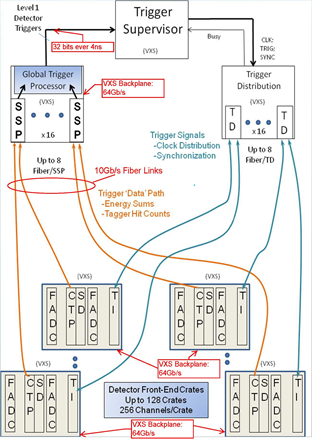
\includegraphics[width=1.0\columnwidth,keepaspectratio]{img/hardware_diagram.png}
	\caption{Hardware diagram with the implemented fiber links scheme.}
	\label{fig:hardwarediagram}
\end{figure}


\subsection{VXS/VME crates}

Previous experiments with the original CLAS spectrometer (see \cite{clas-nim}) used the VXI standard, which was a new extension of the original VME standard. VXI offered a method to distribute clock and other timing signals with low skews via the back-plane. 9U circuit boards were used that offered a large number of front panel input/output connections to handle the six sectors of the CLAS detectors that contributed to the level 1 trigger. The detector signals were acquired with FastBus ADC and TDC or in some instances, from VME or even CAMAC modules. 

During the initial design phase of the 12~GeV experiments the requirements of a 200~KHz sustained trigger rate demanded that the front-end modules adopt a new method of handling precision timing and synchronization over dozens of front-end crates. The latest technology at the 12~GeV inception included FPGA devices with high-speed serial transceivers built into the silicon fabric. A new VME extension was also emerging at the same time, which was labeled VXS, and defined a new high-speed gigabit connector with links between the VME slots and eight serial links to common switch slots. The VXS standard was declared as VITA 41 and several new standards have emerged in the past decade that expand the use of gigabit serial transmission via the crate back-plane. For the 12~GeV experiment era, we now have thousands of custom VXS payload and switch slot modules and hundreds of VXS front-end crates. Complex experiments and high channel count detectors make use of these custom VXS boards  designs for all four experimental halls at JLab.

\subsection{VME Crate Controllers}

The high-speed data physics acquistion and trigger systems for the JLab 12~GeV experiments have been standardized on the VME64X and VXS backplane and crate enclosure form-factor. In addition to the custom electronics that reside in these crates, there must also be a single ``controller'' for each crate. Considering all four experimental halls, this exceeds 100 controllers.

There are many commercial off-the-shelf options for this type of controller, and our general requirements do not extend beyond what is currently commercially available. We do have some specific requirements that narrowed the viable choices.

We purchased VME controllers from several vendors for development purposes and made a significant investment in custom software that runs on all of the existing boards. We also benchmarked our code and have come to expect certain ``minimum'' requirements for performance from the chosen architecture within an specified Linux operating system.

We also expect a certain minimum 10 year timeframe in which these controllers will be supported by the vendor with respect to the avilable parts, repair, and software updates. VME controller requirements are summerized in following list:

\begin{itemize}
	\item Single slot VME form-factor - no required rear transition module
	\item Intel Core i7 dual or quad core embedded processer 2~GHz (or greater)
	\item Hyperthreading and 64~bit arch support
	\item 4 GBytes DDR3 (1066~MHz) ECC SDRAM (or greater)
	\item Front panel gigabit ethernet and serial port console
	\item 1 x4 PCI Express XMC expansion slot (or greater)
	\item VME320-interface using the Tundra Tsi148 chip
	\item support for all VME transfer modes including 2eSST
	\item VXS optional: interface supporting both VITA 41.3 (Gig E) and 41.4 (PCIe) standards.
\end{itemize}

After several different boards were evaluated we purchased XVR16 Intel forth Generation 4-core i7-based rugged VME single board computers from GE (see Fig.~\ref{fig:XVR16diagram}). They were installed in the 70+ crates for CLAS12 and have demonstrated excellent performance and reliability. Most of the controllers send data over their built-in 1~GBit link, while for few of them, a 10~GBit daughter board was installed to increase the bandwidth. The maximum data rate from a single crate in CLAS12 never exceeds 130~MB/s, and with that rate 4-core controllers are able to handle the VME data polling, data processing, and sending data over the network without any issues. 

\begin{figure}[hbt]
	\centering
	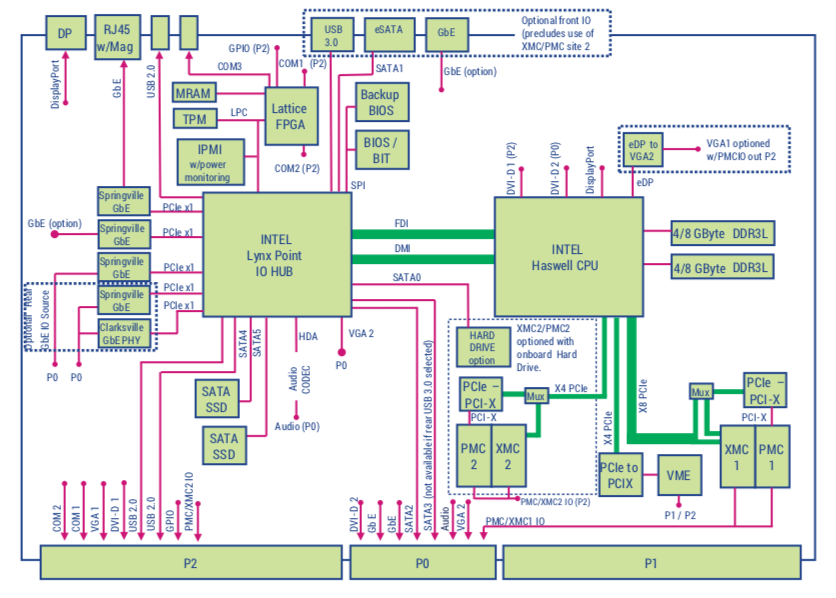
\includegraphics[width=1.0\columnwidth,keepaspectratio]{img/XVR16_diagram.png}
	\caption{Block diagram of the XVR16 VME crate controller}
	\label{fig:XVR16diagram}
\end{figure}



\subsection{Trigger Distribution System Modules (TS, TD, TI)}
	
The TCS (TRIGGER, CLOCK, SYNC, and BUSY) distribution system \cite{tcs-ref} is the hardware interface to bridge the trigger and the DAQ.  The TCS system receives the trigger decision from the trigger system, and initiates data readout for the DAQ system by distributing the readout trigger (TRIGGER) signal.  Additionally, it distributes a 250~MHz system clock (CLOCK) to pipeline the system, and it distributes an encoded synchronous signal (SYNC) for the system synchronization.  It monitors the frontend electronics’ status (BUSY) and makes sure of the smooth data readout of the experiments. Fig.~\ref{fig:TCSdiagram} shows a diagram of the trigger and TCS distribution.

\begin{figure}[hbt]
	\centering
	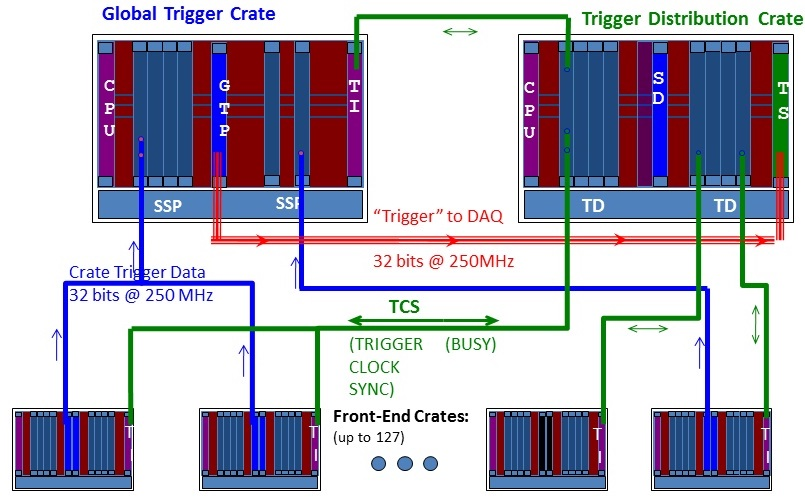
\includegraphics[width=1.0\columnwidth,keepaspectratio]{img/TCSdiagram.jpg}
	\caption{Diagram of the trigger and TCS distribution. The VTP boards generate triggers using detector signals from the front end crates.  The final trigger decisions, up to 32 trigger types, are sent from VTP to TS for data readout.  The TS distributes the TCS to the TD through SD and the backplane, then to the front end crate through optic fiber and TI.  The TI collects the front end boards busy signals and sends to TD, then throttle (disable) the readout trigger distribution on TS.
}
	\label{fig:TCSdiagram}
\end{figure}


The main hardware of the TCS distribution system includes a Trigger Supervisor (TS \cite{ts-ref}) board (see Fig.~\ref{fig:TSused} and ~\ref{fig:TSdiagram}), Signal Distribution (SD \cite{sd-ref}) boards, Trigger Distribution (TD \cite{td-ref}) boards  (see Fig.~\ref{fig:TDused}), Trigger Interface (TI \cite{ti-ref}) boards  (see Fig.~\ref{fig:TIused} and ~\ref{fig:TIdiagram}), VXS crates, and optic fibers.  The TS board, one SD board, and up to sixteen TD boards are located in the global TCS distribution VXS crate.  One TI board and one SD board and/or one FANIO board are located in each front-end crate.  The electronics boards were custom designed and produced for the 12 GeV upgrade.  Field Programmable Gate Arrays (FPGA) are used for TCS generation, control, and decoding.  Optical fibers and high-speed differential backplane connections are used to transmit signals at high speed over long distances.  

\begin{figure}[hbt]
	\centering
	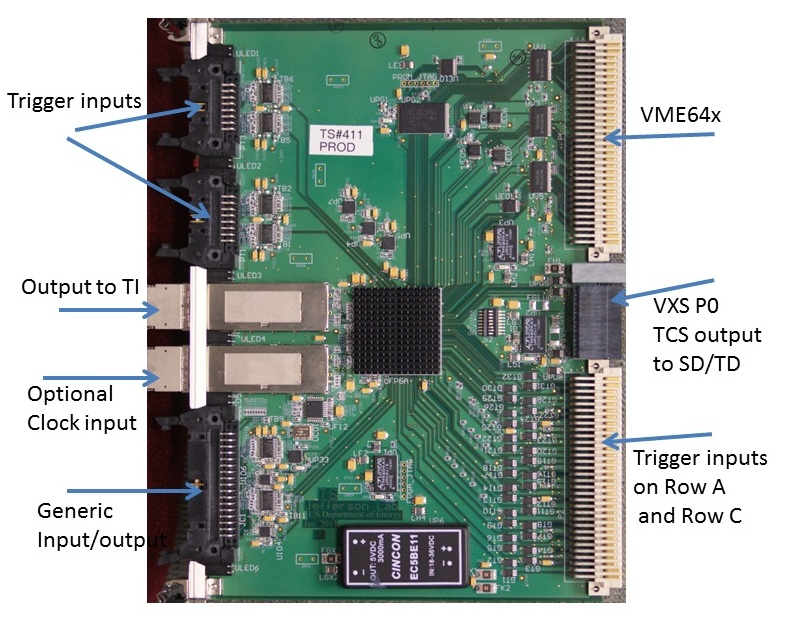
\includegraphics[width=1.0\columnwidth,keepaspectratio]{img/TSused.jpg}
	\caption{Trigger Supervisor (TS) board.  The TS board is a 6U by 160mm VME board with VXS connector.  It generates and distributes the readout triggers, synchronization signals, and clock (either from the front panel input or the on-board oscillator) to the TD boards via the SD through the VXS backplane.}
	\label{fig:TSused}
\end{figure}

\begin{figure}[hbt]
	\centering
	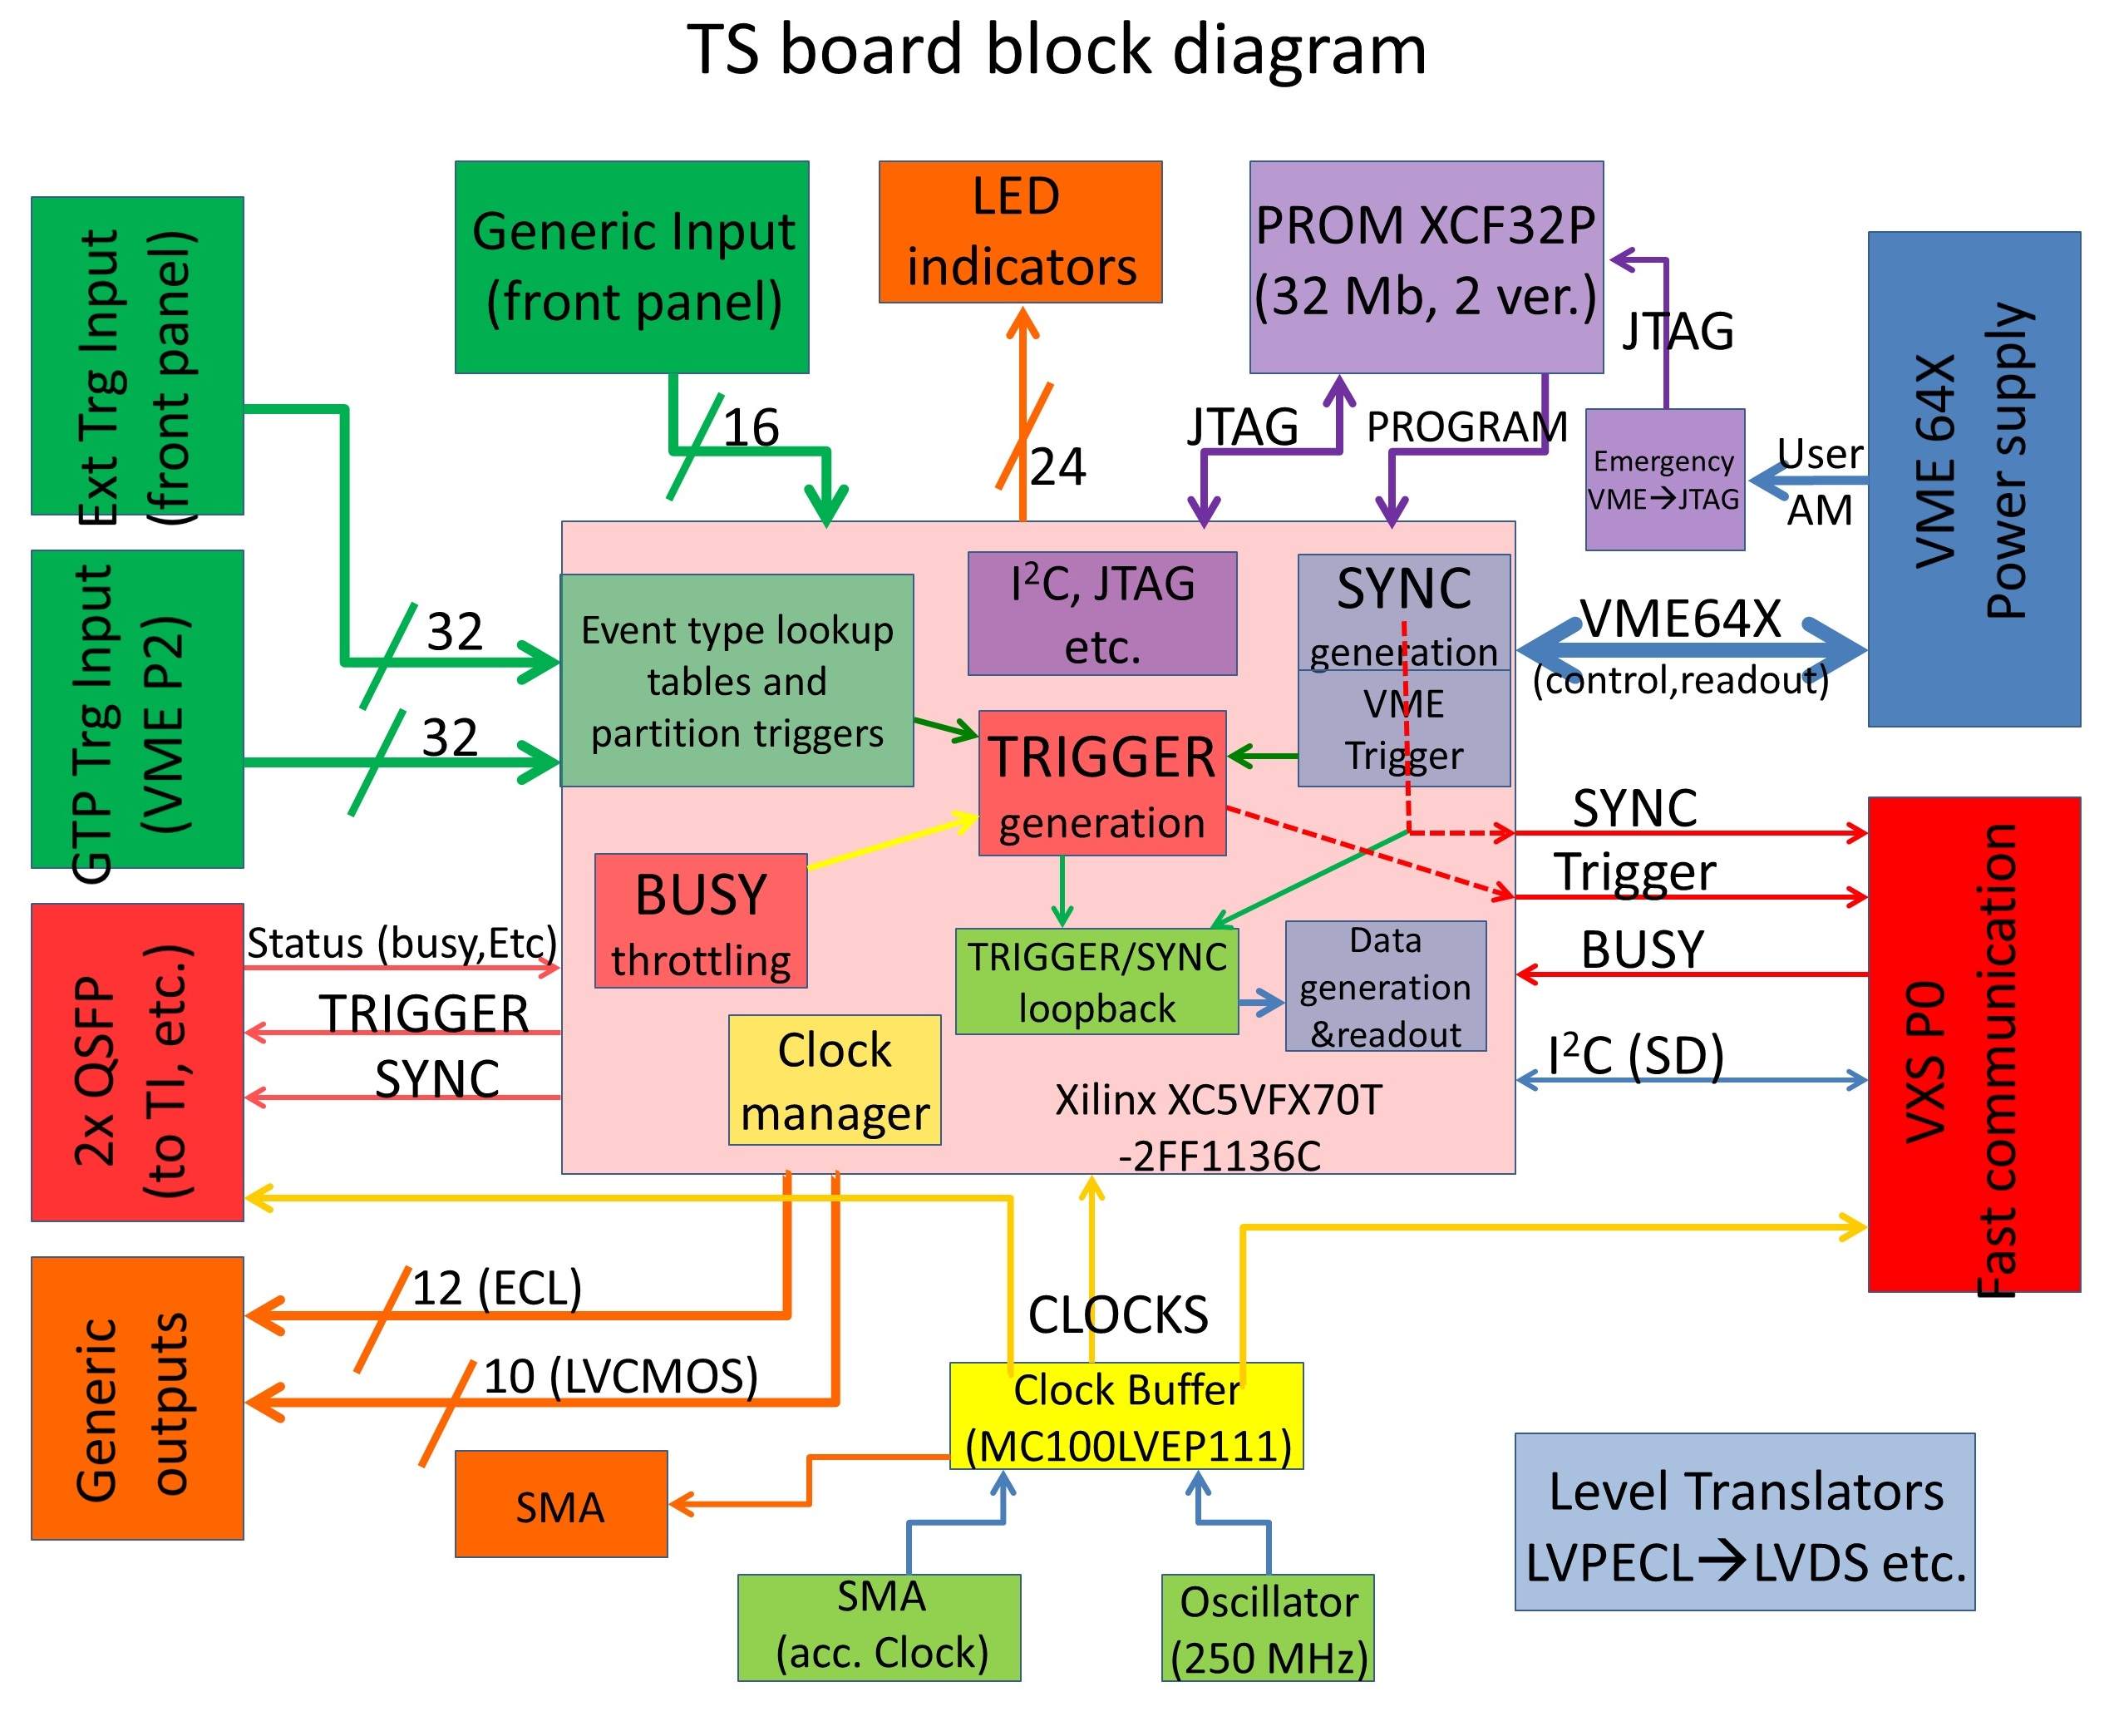
\includegraphics[width=1.0\columnwidth,keepaspectratio]{img/TSdiagram.jpg}
	\caption{TS board diagram.  The TS generates the readout triggers from up to 32 front panel trigger inputs and up to 32 backplane trigger inputs (from GTP), and sends out the triggers via encoded 16-bit words to the backplane.}
	\label{fig:TSdiagram}
\end{figure}

\begin{figure}[hbt]
	\centering
	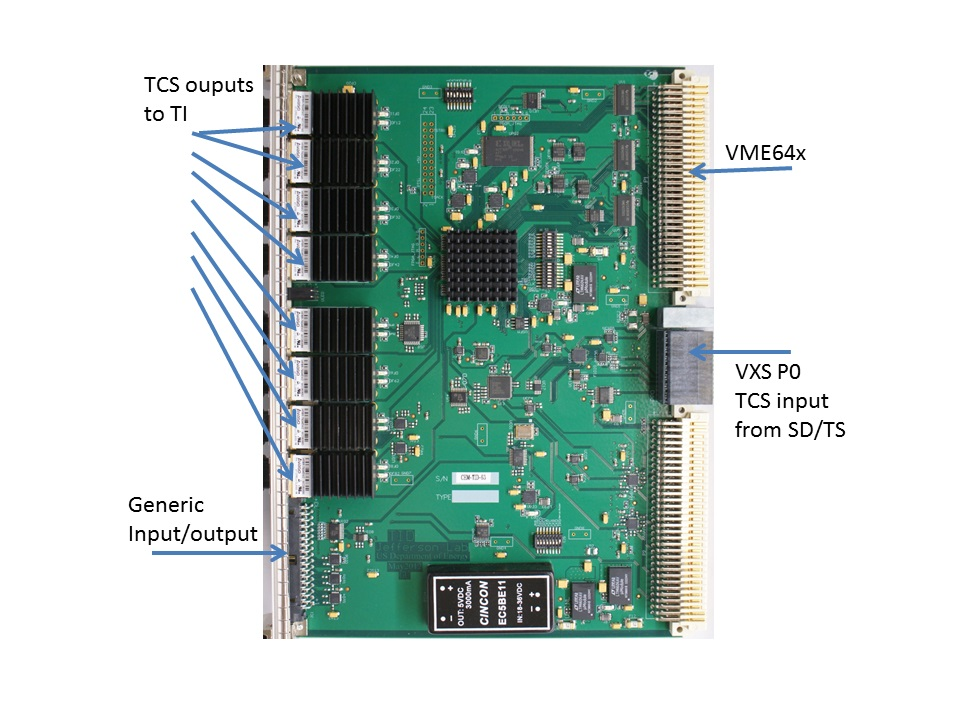
\includegraphics[width=1.0\columnwidth,keepaspectratio]{img/TDused.jpg}
	\caption{Trigger Distribution (TD) board.  The TD board is a 6U by 160mm VME board with VXS connector.  It receives the TCS from TS via the VXS backplane, and distributes the TCS via the front panel QSFP optic links.  It collects the Busy inputs from up to eight TI boards, and generates the readout buffer busies for up to eight front end crates.  The TD sends the collective BUSY to TS to back pressure the trigger generation.}
	\label{fig:TDused}
\end{figure}

\begin{figure}[hbt]
	\centering
	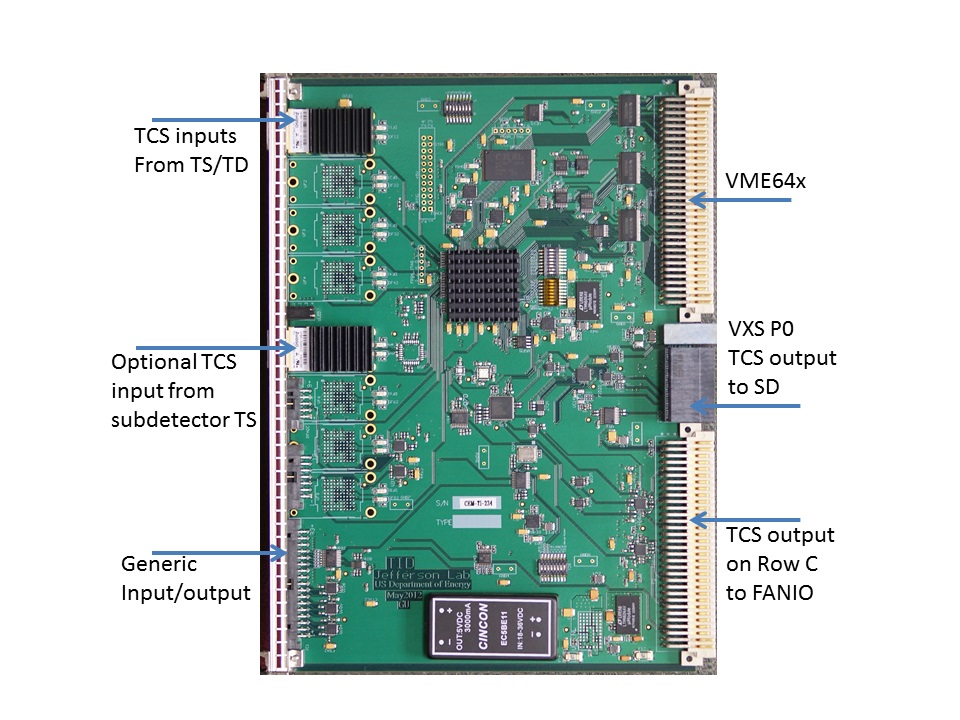
\includegraphics[width=1.0\columnwidth,keepaspectratio]{img/TIused.jpg}
	\caption{Trigger Interface (TI) board.  The TI board is a 6U by 160 mm VME board with (or without) the VXS connector.  It is using the same PCB as TD board with modified components population.  It receives the TCS from TS/TD or a sub-system controller via fiber, and collects the busy and sends to TS/TD via the same fiber.  The TI can also be used as a subsystem controller in the so-called master mode.}
	\label{fig:TIused}
\end{figure}

\begin{figure}[hbt]
	\centering
	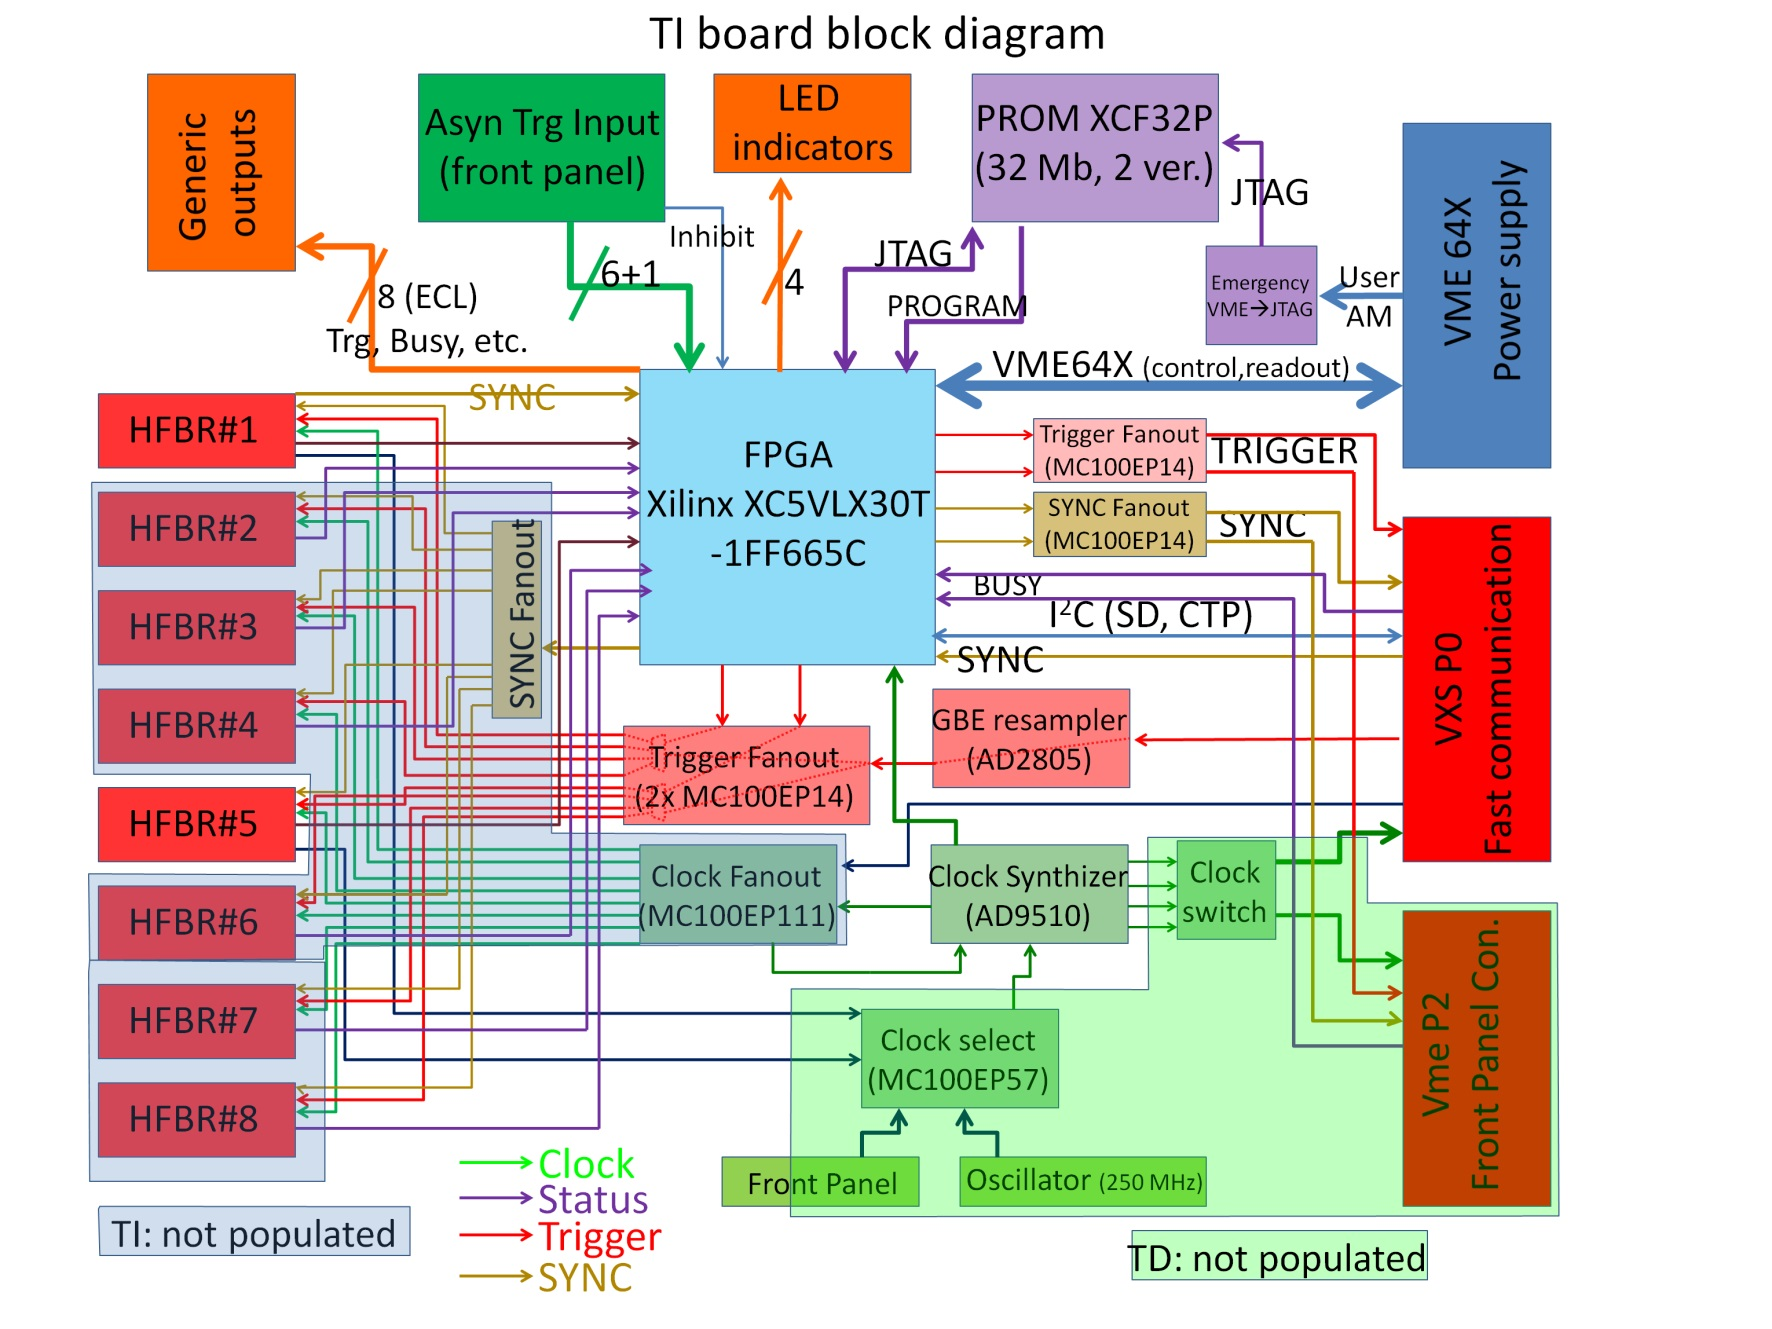
\includegraphics[width=1.0\columnwidth,keepaspectratio]{img/TIdiagram.jpg}
	\caption{TI and TD board diagram.  The TI and TD use the same PCB design, but different component population and FPGA firmware.}
	\label{fig:TIdiagram}
\end{figure}


\subsubsection{Clock Distribution}

The TCS system uses the 250 MHz clock, that comes from the TS in the global trigger distribution crate.  This clock is either generated by the TS on-board oscillator or its fronts panel input.  The clock is fanned out to the VXS P0 connector and then to the SD board.  The SD fans out the clock to the TD boards via the VXS P0 backplane.  The TD boards further fan out to the TI boards via optic fibers.  The TI uses this clock to generate clocks with proper frequencies (250 MHz, 125 MHz, 62.5 MHz, 31.25 MHz and 41.67 MHz) and sends the clocks to the front-end crate SD board, and the SD fans out to the front-end DAQ modules (TDC, ADC).  The fan-out buffer level is minimized on every board to limit the clock jitter.  The slower clocks derived from the main system clock are phase aligned thanks to the Analog Devices AD9510 with a synchronous phase re-alignment command.  The clock jitter is about one ps measured at the front-end electronics.  The clock distribution skew can be adjusted by the SD clock delay if necessary.


\subsubsection{SYNC Distribution}

The TS generates and distributes the SYNC signal.  The SYNC is an encoded 4-bit serialized command transferred at 250 Mbps synchronized with the system clock.  Normally, the serial SYNC line stays at logic high (or ‘1’).  When transferring a SYNC command, the SYNC goes to logic low for one bit, followed by the 4-bit command code.  After the 4-bit SYNC command, the SYNC goes to logic high again.  There is a minimum of four ‘1’s before the next cycle begins.  The SYNC start is phase aligned to the 62.5 MHz clock used for the trigger word transfer, the 41.67 MHz clock used for the CAEN TDC boards, and the 31.25 MHz clock used for Flash ADC boards.  This phase relation is used to synchronize the slower clocks on the TI to the 62.5 MHz clock on the TS.  This also limits the SYNC command to no more than one per 96 ns.  To facilitate the AC coupled optical transceivers, the SYNC is Manchester encoded on the TS and the TD, and Manchester decoded on the TI and the TD.

The SYNC is phase aligned with the 250 MHz system clock on the TI boards using their FPGA’s IODELAY.  The SYNC is synchronized across the TI boards by applying different delays on the individual TI boards.  The delays are determined by the fiber latency measurement.  

The spare fibers between the TD and TI boards are used to measure the fiber latency.  The TI sends a test signal to the TD through one fiber, and the TD loops back the signal through another fiber.  The TI measures the delay between the test pulse and the looped back test pulse using the FPGA counter and the carry chain in the FPGA.  As the fiber skew is small (less than 1 ns for 100 meter fibres), the measurement on these two fibres can be used as the latency of the other fibres in the cable.  
After the SYNC latency compensation, all the TI boards receive the SYNC at the same time with the skew of one system clock period, which is 4 ns.  The synchronized SYNC signals are used to synchronize the triggers as described next.


\subsubsection{Trigger Distribution}

The trigger words, which include the readout trigger signals and event information (event type, trigger timing, etc.), are generated and serialized on the TS.  The serialized trigger word is fanned out by the SD board and the TD board, and deserialized by the TI board.  The 16-bit trigger words are summarized in Table~\ref{tab:trigger_word_definition}.  

\begin{table}
\begin{adjustbox}{width=\columnwidth,center}
	\begin{tabular}{| l | l | l | l |}
		\hline \hline
		Bit 15:12		& 	Bit 11:10 &	Bit 9-0	 & Comment		\\
		\hline
	1001	& Quadrant timing	& Event type	 & GTP major trigger \\
	1010	& Quadrant timing	& Event type	 & Ext major trigger \\
	
	1011	& \multicolumn{2}{c}{Four TS partitions’ event types}    & TS partitioning (4, 3, 2, 1) \\

	\multirow{2}{*}{0110}	& \multirow{2}{*}{Quadrant timing}	& Trigger source & TImaster legacy Trigger \\
		    &                   & Event type	 & (TS) VME trigger     \\
	0101	& Trigger command/Control	& VME command \\
	0100	& TS timer (TS time bit(13:2))	& TI Sync check \\
	0111	& Trigger content	& Additional trigger info \\
		\hline \hline
	\end{tabular}
\end{adjustbox}
\caption{Trigger word definition.  The TS encode the readout trigger, event type, and the fine timing (4ns quadrant) information into a 16-bit word, which is transferred every 16ns.  This 16-bit word can also be some system setting information or the system timer when there is no readout trigger in the 16ns periods.}
\label{tab:trigger_word_definition.}
\end{table}

Both the fiber latency and trigger word serializer/ deserializer are compensated so that all the TI boards send the readout trigger at the same time to the front-end data acquisition electronics.  The SYNC is used in conjunction with a synchronous FIFO to enforce a fixed latency on the trigger distribution. Fig.~\ref{fig:TIsync} shows the diagram of the compensated trigger distribution.

\begin{figure}[hbt]
	\centering
	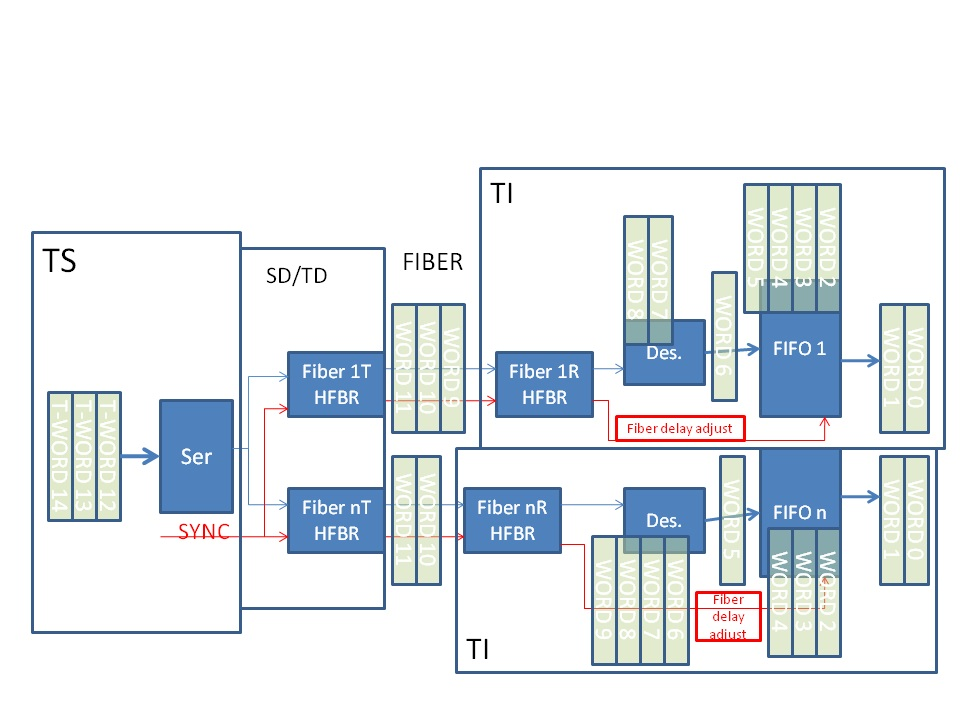
\includegraphics[width=1.0\columnwidth,keepaspectratio]{img/TrgSync.jpg}
	\caption{Trigger synchronization between TIs.  The TI boards delay the decoding of the received readout trigger by the complement of the TS/TD to TI transfer latency, so that all the front end boards receive the readout trigger simultaneously.}
	\label{fig:TIsync}
\end{figure}

On the TI board, the deserialized trigger word is clocked into and clocked out of a FIFO using the 62.5~MHz clock.  At the start-up, the FIFO is reset (0 words) and the FIFO read/write is disabled.  The serial trigger link is idle words only.  On trigger start, the TS starts trigger word transmission.  The TI will write the deserialized data (valid data, that is non-idle data word) to the FIFO.  After some pre-set delay (VME register controlled), the TS issues a ‘Trigger Start’ command on the SYNC link.  When TI receives the ‘Trigger Start’, the TI resets the trigger FIFO readout address, and enables continuous readout of the FIFO.  As the SYNC lines are fiber length adjusted and the 62.5 MHz clocks are phase aligned, the trigger words from the TI board FIFO are synchronized across the system.
The trigger word also has the fine trigger timing information.  By decoding that, the TI board distributes the trigger in 4 ns precision, although the trigger word is serialized every 16 ns.  If the system clock phase is not adjusted, there will be a maximum of 4 ns skew among the clocks on the TI boards, so does the readout trigger.  The clock phase can be adjusted by SD if the skew is critical to the system.


\subsubsection{DAQ synchronization (trigger throttling) control}

Because of the finite memory size and the randomness of the triggers, it is possible for the memory to become overwhelmed somewhere in the system, which could cause DAQ problems.   The TCS throttling mechanism is used to prevent possible memory overflows, and to keep the DAQ synchronized.  Fig.~\ref{fig:DAQ_synchronization} shows the DAQ synchronization logic implementation.  Three methods are used to keep the DAQ synchronized.  These include trigger rules and event limit setting, pipeline DAQ, and synchronization events (special events).

\begin{figure}[hbt]
	\centering
	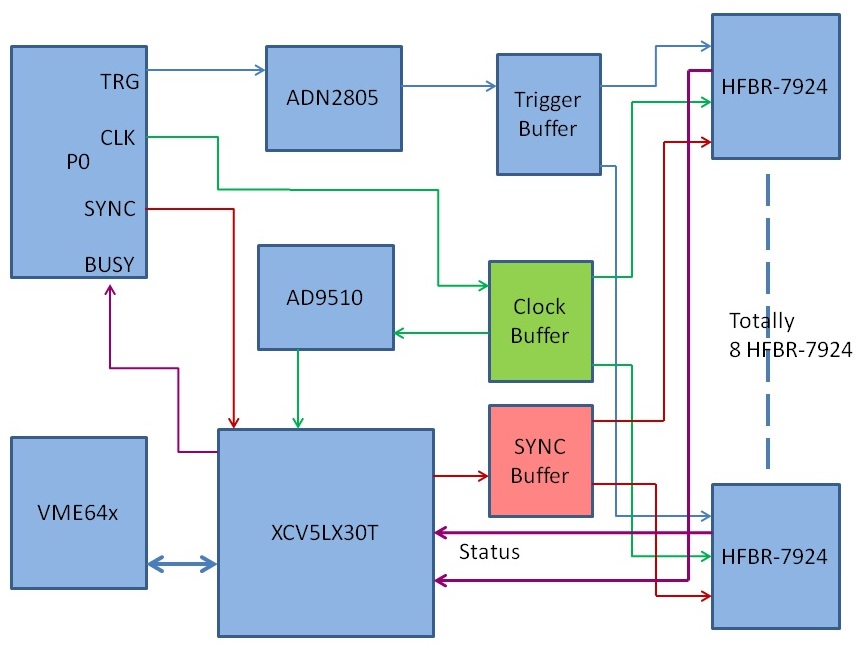
\includegraphics[width=1.0\columnwidth,keepaspectratio]{img/TDdiagram.jpg}
	\caption{DAQ synchronization}
	\label{fig:DAQ_synchronization}
\end{figure}


%REFERENCES
%[1] 	J. Gu etal. (2014, May). The TRIGGER/CLOCK/SYNC Distribution for TJNAF 12 GeV Upgrade Experiments    %https://coda.jlab.org/wiki/index.php/Trigger_distribution_overview
% [2] 	J. Gu. Description and technical information for the Trigger Supervisor (TS) module.  TJNAF, VA, 2013.  %Available: https://coda.jlab.org/drupal/system/files/pdfs/HardwareManual/TS/TS.pdf 
%[3] J. Gu, etal, 	“Design of the Trigger Interface and Distribution Board for TJNAF 12 GeV Upgrade,” IEEE Trans. Nucl. %Sci., Vol. 60, no. 5, pp 3714-3719, Oct. 2013

	
\subsection{Signal Distribution Module (SD)}

The Signal Distribution Board (SD \cite{sd-ref}) module (see Fig.~\ref{fig:SDpic}) occupies the “B” switch card slot as specified in VITA 41. The main purpose of this module is to distribute the signals received from payload slot 18 (Trigger Interface board) of a VXS crate to the 16 other payload slots (ADC boards).

The SD module distributes the 4 LVPECL differential pair  signals from payload slot 18 to 16 VXS payload slots within the crate. This is done using the high-speed, point-to-point connections from the switch slot to each payload slot. The four distributed signals are length-matched to minimize the output jitter seen on all of the payload slots. Three of the four remaining pairs are LVDS signals routed from the each payload module to the FPGA on the SD module. The last pair is an LVDS signal routed from the FPGA on the SD module to each payload module. Each of the 16 payload modules has a single-ended signal to the SD module and one from the SD module back to the payload module.

\begin{figure}[hbt]
	\centering
	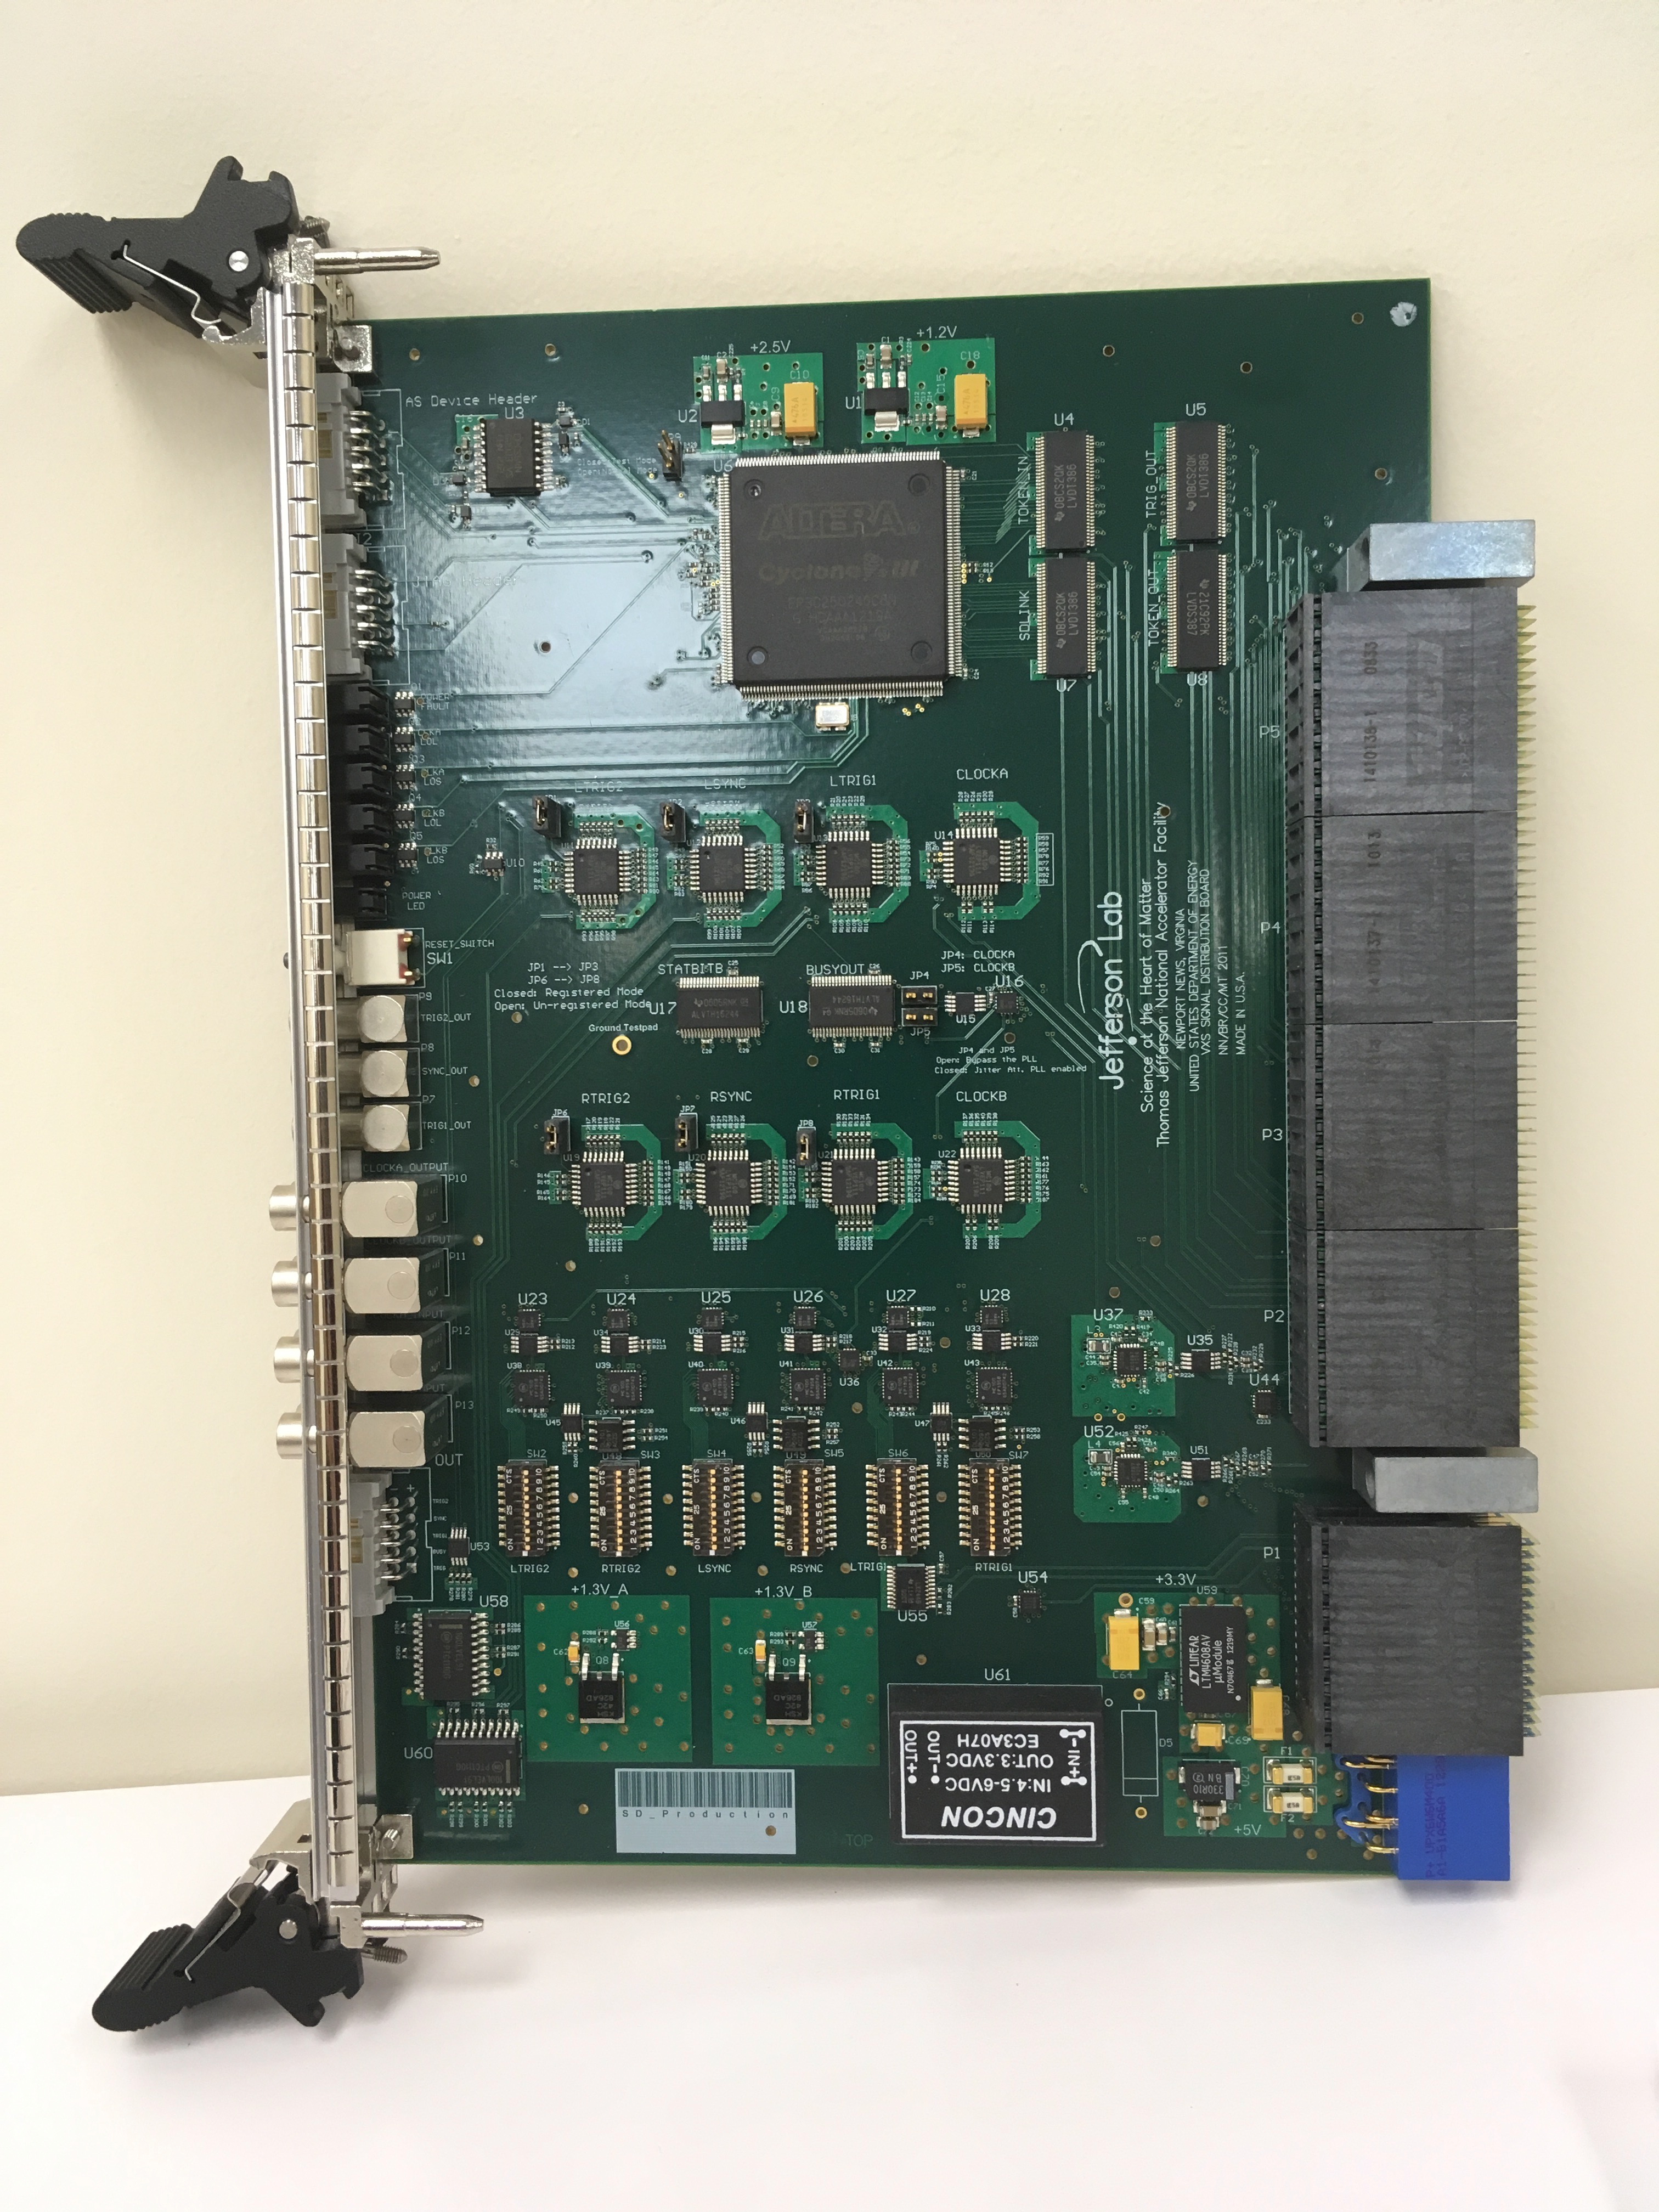
\includegraphics[width=1.0\columnwidth,keepaspectratio]{img/sd_board.jpg}
	\caption{Signal Distribution module (SD)}
	\label{fig:SDpic}
\end{figure}


\subsection{Flash ADC Module (FADC250)}

A 16-channel 250 MSPS pipelined flash ADC (FADC \cite{fadc-ref}, see Fig.~\ref{fig:FADC250pic}) with 12-bit precision was designed to digitize and process detector pulses for experiments at JLab.  The FADC250 module (see Fig.~\ref{fig:FADC250_board}) conforms to the VITA-41 VME64x switched serial (VXS) standard.  Each channel of the module accepts input signals on a LEMO style coaxial connector and has three user-selectable ranges (0.5 V, 1.0 V, 2.0 V).  Differential signal conditioning scales the input signals to within the dynamic range of the ADC and a single-pole low pass filter limits the signal bandwidth to the Nyquist band of the converter (125 MHz). Individual channel offsets are accomplished by means of DACs under VME control.  Each channel has its own dedicated ADC chip (Analog Devices AD9230). Both positive and negative polarity input signals are supported. The 250 MHz clock is distributed to the ADC chips through a low jitter ($<$ 2~ps) network.  

\begin{figure}[hbt]
	\centering
	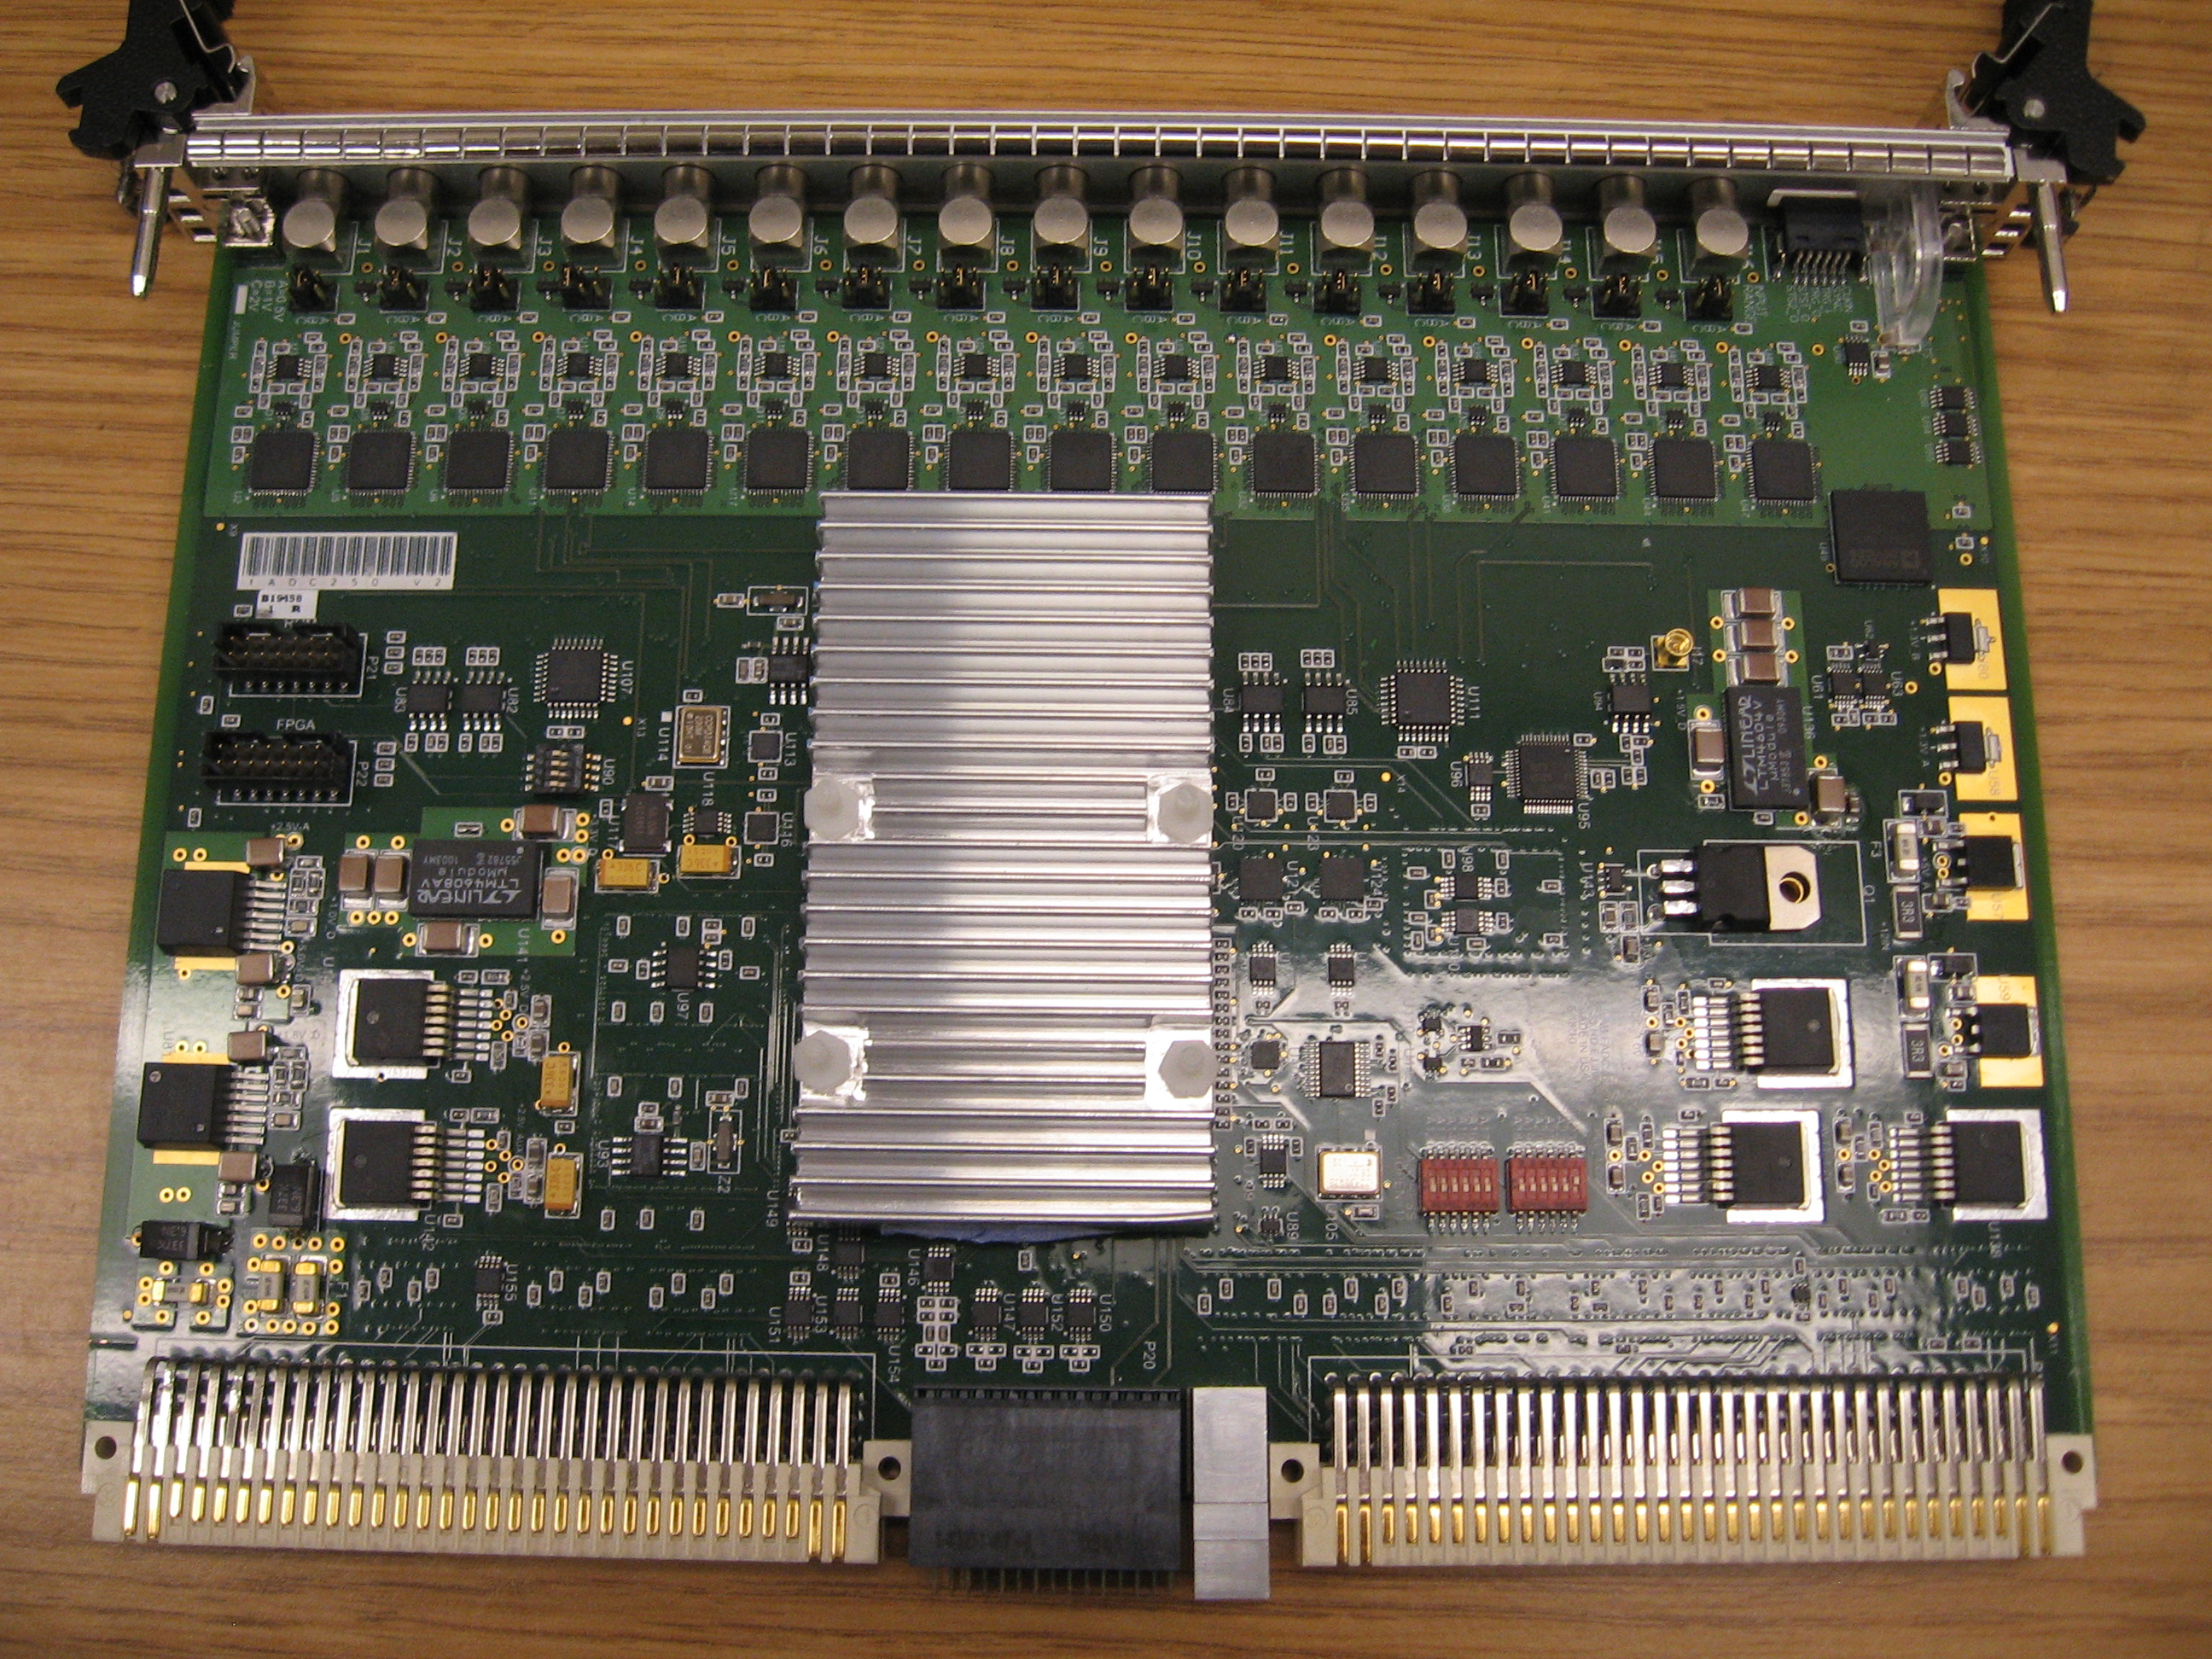
\includegraphics[width=1.0\columnwidth,keepaspectratio]{img/FADC250pic.jpg}
	\caption{Flash ADC module (FADC250)}
	\label{fig:FADC250pic}
\end{figure}

\begin{figure}[hbt]
	\centering
	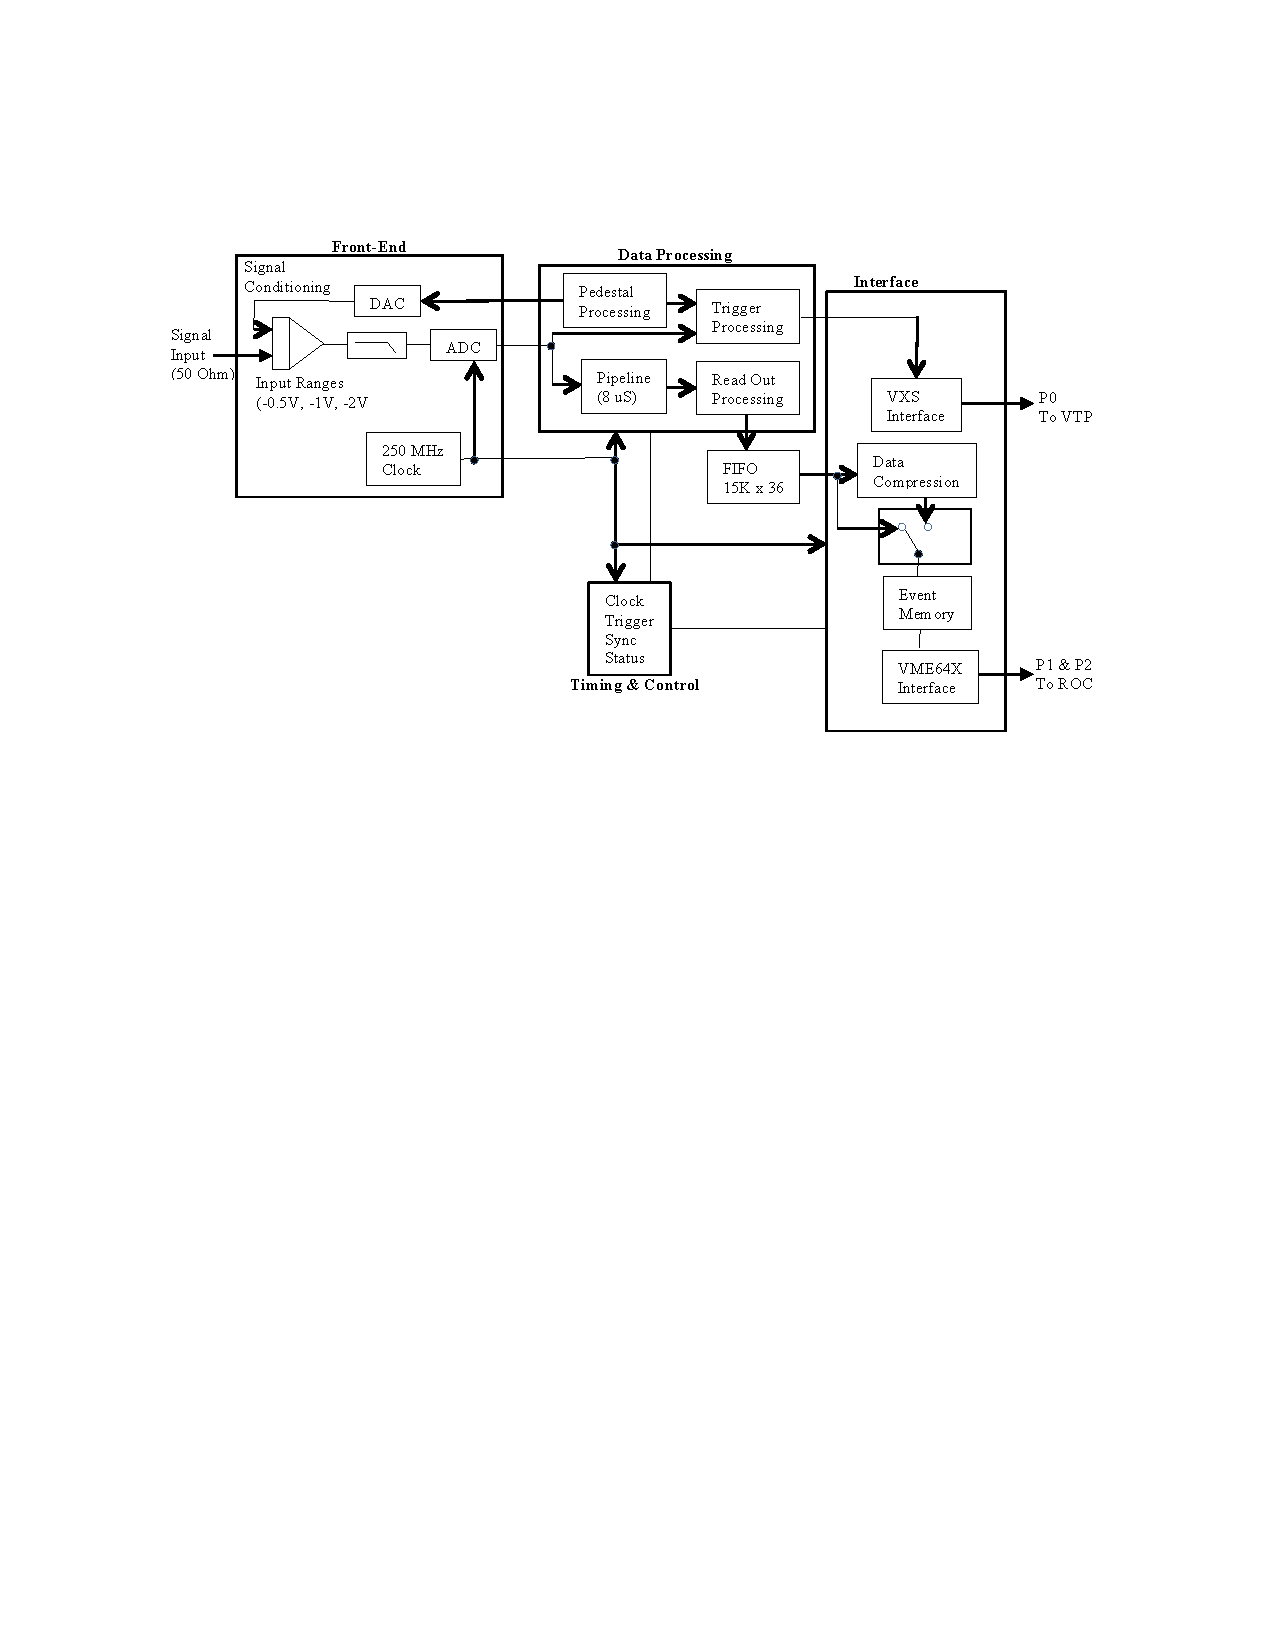
\includegraphics[width=1.0\columnwidth,keepaspectratio]{img/FADC250_Diagram.pdf}
	\caption{Flash ADC module diagram (FADC250)}
	\label{fig:FADC250_board}
\end{figure}

Digitized data from the 16 FADC chips is processed and formatted for readout in a pair of high performance Xilinx FPGAs. The digitized data from the ADCs follows two distinct paths.  Logic in the trigger data path pre-processes data for the trigger algorithms of the VXS Trigger Processor (VTP). The FADC250 module continuously streams this data to the crate VTP located in VXS switch slot A via high-speed serial links of the VXS fabric.  Data from multiple VTPs and other modules are used to form a global trigger signal that is returned to the crates to initiate data readout.

The readout data path continuously stores digitized data for each channel in circular buffers. When a trigger signal is received by the module a programmable window up to 2 $\mu$s wide of digitized data is extracted from the buffers for processing. The starting point of this window can be programmed up to 8 $\mu$s earlier than the arrival of the trigger signal to account for the time required to form the trigger signal.  Zero suppression on the extracted data may be implemented for each channel using programmable thresholds.  A lossless data compression algorithm can also be applied to the data of each channel with typical compression factors of 2 to 3. The design is pipelined so that data from multiple triggers can be processed simultaneously.  Triggers separated in time by as little as 50 ns can be accepted by the module. The trigger number and trigger time (clock periods since last synchronization) are reported along with the channel data so that data from multiple modules can be correctly assembled into events. 

Data associated with a programmable number ``N'' of triggers is packaged into a block of data for read out over VME.  ``N'' can take values from 1 to 255, with 40 being a typical value chosen.  Data is stored in an on-board 8 MB SRAM as 64-bit words to match the 64-bit high-speed (200 MB/s) dual edge VME Source Synchronous Transfer (2eSST) mode employed to read out the module.  

In order to save the overhead of setting up a DMA transfer for each FADC250 module in the crate, a chained block readout mechanism with token passing is used.  A common address range is enabled for all modules in the crate but only the module having the token will respond to a read request.  A single logical DMA read is initiated by the VME crate controller and the first module in the chain supplies data from its block of event fragments.  When the block data from the first module is exhausted, a token signal is passed to the next module in the chain and this module then proceeds to transmit its data from its block.  When the block for the data from that module is exhausted, it transfers the token to the next module.  This continues until the data from the last module in the chain is exhausted.  Instead of passing the token the last module asserts the VME bus error signal (BERR), which terminates the DMA cycle.  The user returns the token to the first module and the process can begin again when the next block of events is ready for readout.  The user does not have to query the modules in advance to discover the number of words to read out.  The DMA is set up with a total number of words larger than any expected value for the entire crate.  Data from each module is tagged with the slot number to identify its source.  The token passes along a VXS signal line to VXS switch slot B, where a module there (SD) routes it to the next enabled module.


\subsection{Discriminator Scaler Module (DSC2)}

The Discriminator Scaler Module (DSC2 \cite{dsc2-ref}, see Fig.~\ref{fig:dsc2_board}) is a 16-channel general purpose discriminator and scaler module designed as a 6U VME card. It replaces an older design, improving on jitter, noise, crosstalk, and adding new features.

\begin{figure}[hbt]
	\centering
	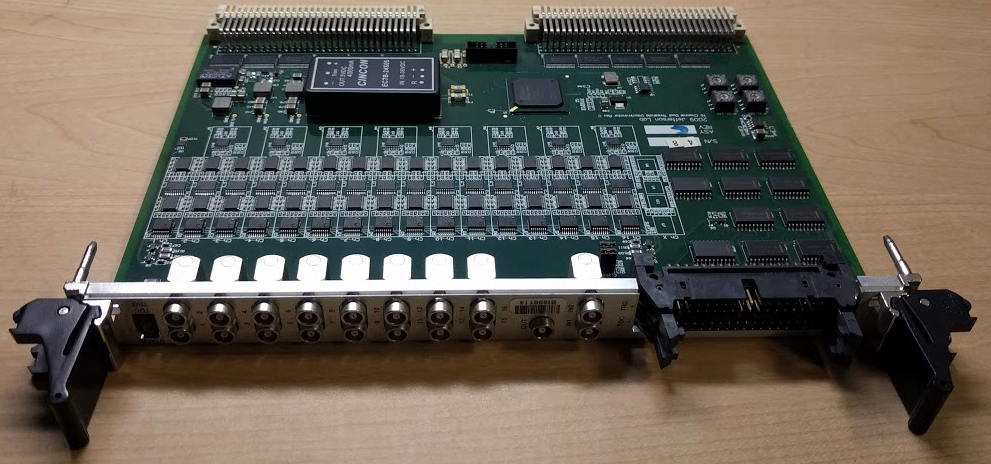
\includegraphics[width=1.0\columnwidth,keepaspectratio]{img/dsc2_board.png}
	\caption{Discriminator Scaler module (DSC2)}
	\label{fig:dsc2_board}
\end{figure}

\begin{center}
	DSC2 Specifications\\
	\begin{tabular}{| l | l |}
		\hline \hline
		Property			& Value				\\
		\hline
		{\bf Analog Discriminator}	&				\\
		Threshold			& 0 to -1023 mV			\\
		Pulse width			& 4 ns to 40 ns			\\
		Dead-time			& 4 ns typ. w/8 ns pulser width	\\
		Maximum input rate		& $>$125 MHz 			\\
		Ch-ch isolation			& $>$65 dB			\\
		Threshold noise			& 1.3 mV RMS (typical)		\\
		Slew-rate delay disperson	& $<$20 ps			\\
		Input-to-output delay		& $<$5 ns			\\
		{\bf Digital Processing}	&				\\
		Digital delay step		& 4 ns				\\
		Digital delay maximum		& 1 us				\\
		Digital width maximum		& 1 us				\\
		Maximum count rate		& 125 MHz			\\
		\hline \hline
	\end{tabular}
\end{center}

\paragraph{Discriminator}
Inputs are single-ended LEMO and leading-edge discrimated by two different thresholds. Typically one threshold is used for time-to-digital applications and the other threshold is used for trigger applications. There are separate differential ECL outputs for each channel and threshold. Low jitter performance was an important goal of the design as this module will be used in high resolution applications. Fig.~\ref{fig:dsc2_jitter} shows the typical jitter as a function of a variety of input slew rate signals and threshold overdrive conditions.

\begin{figure}[hbt]
	\centering
	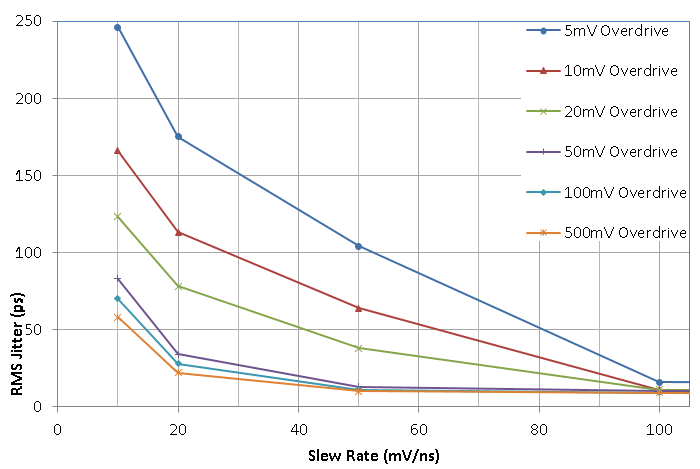
\includegraphics[width=1.0\columnwidth,keepaspectratio]{img/dsc2_jitter.png}
	\caption{Output Jitter vs Input slew rate and overdrive}
	\label{fig:dsc2_jitter}
\end{figure}

\paragraph{Digital Processing}
A Xilinx Spartan 3A FPGA is used to implement the VME interface, scalers, discriminator controls, and scaler event building features. Each channel and threshold has two scalers associated with it. The first scaler counts all threshold crossings for the input. The second scaler is gated using a front-panel input source, which can be useful to computing dead-time of channels and many other applications. Additionally, reference scalers are accumulated (a gated and ungated version) that count the elapsed time, which can be used to normalize inputs scalers to Hz. All together there are 68 scalers, which can be slow to read over VME if using single-cycle transfers. An event builder is implemented that can synchronously read (and optionally clear) all scalers and build an event with this data. Over 100 events can be buffered and readout using the VME 2eSST protocol at 200~MB/s.


\subsection{TDC Modiles (v1190/v1290)}

Commercial CAEN V1190/V1290/V1290N TDC \cite{tdc-ref} boards are used for timing measurements in the PMT-based CLAS12 detectors (see Fig.~\ref{fig:v1190_board}). The V1190 has timing resolution about 100~ps and the V1290 about 35~ps. All boards installed in CLAS12 run on an external 250/6=41.666~MHz clock rather then internal 40~MHz clock. The use of a different clock required compensation table remeasuring and reloading.

\begin{figure}[hbt]
	\centering
	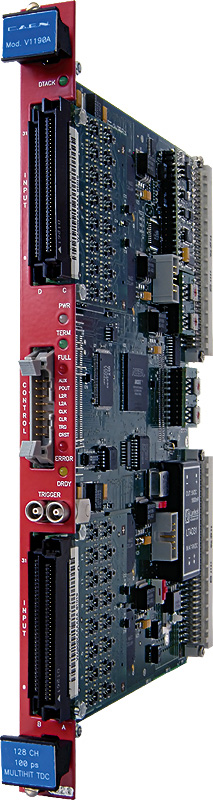
\includegraphics[width=0.2\columnwidth,keepaspectratio]{img/v1190_board.jpg}
	\caption{CAEN V1190 TDC module (V1190)}
	\label{fig:v1190_board}
\end{figure}

\subsection{Drift Chamber Readout Board (DCRB)}

\begin{figure}[hbt]
	\centering
	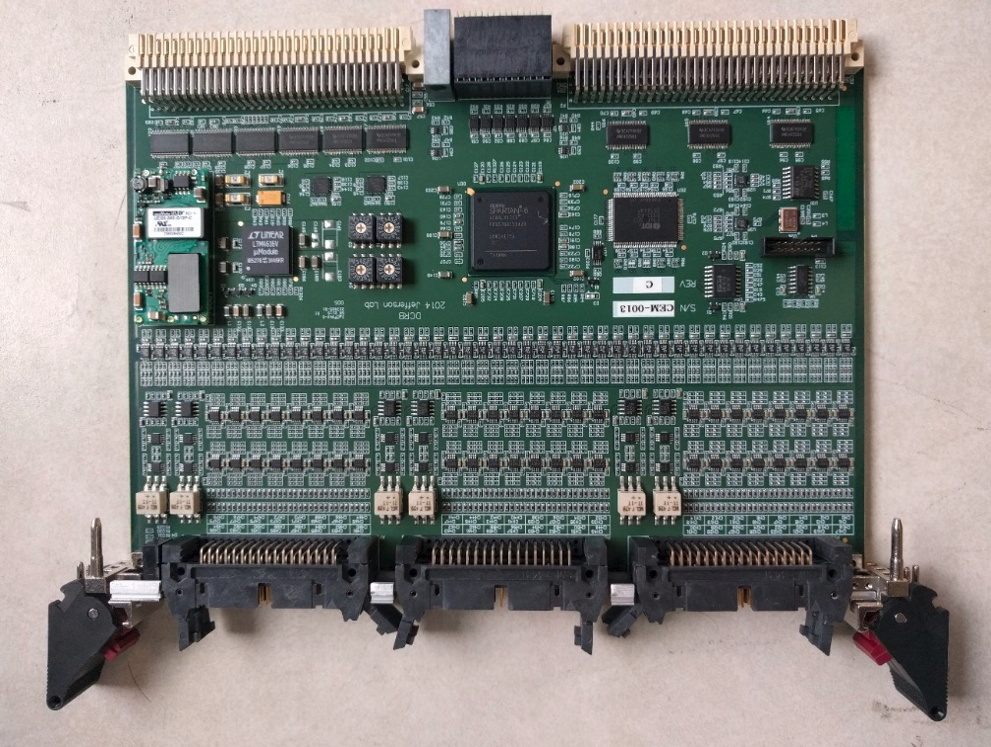
\includegraphics[width=1.0\columnwidth,keepaspectratio]{img/dcrb_board.png}
	\caption{Drift Chamber Readout Board (DCRB)}
	\label{fig:dcrb_board}
\end{figure}

The Drift Chamber Readout Board (DCRB \cite{dcrb-ref}, see Fig.~\ref{fig:dcrb_board}) is a 96-channel amplifier, discriminator, and time-to-digital converter module used to digitize and readout hits from the CLAS12 Drift Chambers. A single VXS crate of DCRB modules can readout a full region of the drift chambers for a single sector resulting in 18 VXS crates of DCRBs to instrument 6 sectors each having 3 regions of drift chamber.

\paragraph{Analog Inputs}
Each DCRB receives 96 differential analog signal pairs using twisted pair cabling from the drift chamber pre-amplifiers. The pre-amplfiers located on the detector provide a gain of ~2.3~mV/$\mu$A. On the DCRB each analog input channel is amplified by a voltage gain of 30 and then discriminated by a programmable threshold (common to all channels on the board with an effective chamber wire threshold range of 0 to 3.5/$\mu$A).

\paragraph{TDC Event Builder}
All discriminated channels go to a Xilinx Spartan 6 FPGA where a 96-channel 1~ns resolution time-to-digital converter (TDC) is implemented in firmware. The TDC is based on the ISERDES2 shift register FPGA primitive that directly samples of the digital input with a single-data-rate (SDR) input register clocked at 1~GHz. The TDC sampling clock is synchronized to the CLAS12 master oscillator, making it easy to relate hit times in the drift chamber to the other detectors in CLAS12. The TDC inputs are buffered to support multiple hits, allowing for an average hit rate of 4~MHz per input before loss of data, which exceeds the chamber design hits rates by a few orders of magnitude. Hits from groups of 16 channels are written into a large buffer that a linked-list content addressable memory (CAM) tracks for 16~$\mu$s. When a L1A trigger signal is received, a time window of hits is extracted from the TDC hit buffer. The readout window times are supplied to the CAM, and the CAM provides the address of the last hit matching each readout time bin. The hit buffer is then read to extract the hit and also the address of the next hit in the buffer matching the time bin (this is the linked list behavior). The result is an extremely fast event builder with natural zero suppression that does not require time sorted data. Cleanup is accomplished by a timer that invalidates the CAM entries after time bins are older then 16~$\mu$s. Hits for an event are assembled and buffered in a 2~MByte external RAM, which is readout through the VME bus using the 2eSST protocol at 200~MB/s.

\paragraph{Calibration Support}
A programmable amplitude pulse generator is implemented that can inject test pulses directly into the DCRB differential amplifier inputs as well as to the pre-amplfiers that are on the detector. This provides a way to test points of failure, check channel gain, and check channel delays without any extra equipment. A scaler is implemented on each channel for slow control monitoring of all chamber wires.

\subsection{VXS Silicon Readout Module (VSCM)}
The CLAS12 Silicon Vertex Tracker detector (SVT, \cite{svt-ref}) front-end utilizes the data driven FSSR2 ASIC for digitization. The VXS Silicon Readout Module (VSCM \cite{vscm-ref}, Fig.~\ref{fig:vscm_board}) was designed to interface the FSSR2-based front-end to the CLAS12 DAQ system. This system is capable of reading out all 33,792 SVT channels in 3 VXS crates.

\begin{figure}[hbt]
	\centering
	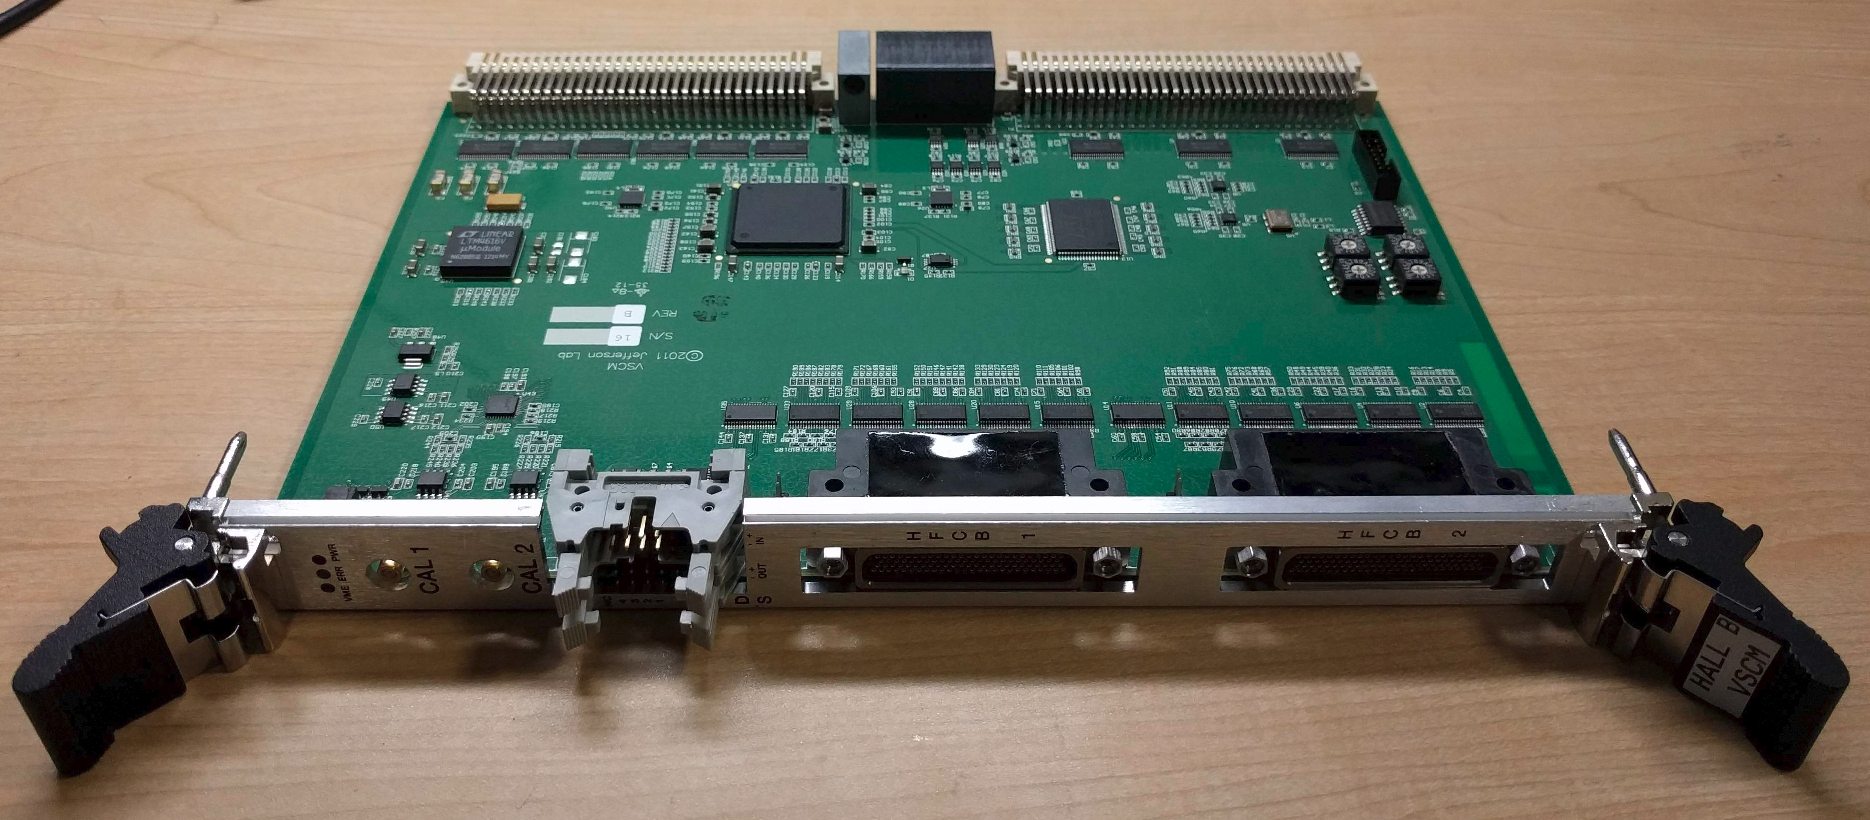
\includegraphics[width=1.0\columnwidth,keepaspectratio]{img/vscm_board.png}
	\caption{VXS Silicon Readout Module (VSCM)}
	\label{fig:vscm_board}
\end{figure}

The main features of the VSCM include:

\begin{itemize}
	\item Receives 8 FSSR2 streams, each at 840~Mbps
	\item De-randomizes hits into an 8~$\mu$s buffer
	\item 512k hit, multi-event buffer
	\item Supports $>$1~MHz trigger rate
	\item Programmable amplitude charge injector
	\item 1~ns resolution time-to-digital converter (TDC)
	\item Per channel hit scaler
	\item FSSR2 synchronization, status, and control
\end{itemize}

\paragraph{Event Builder}
The VSCM deserializes the FSSR2 streams, checks for errors, and decodes the hits, which are stored in an 8~$\mu$s circular memory. The hits are not guaranteed to be time ordered, so the timestamp and channel number are used to form the circular memory address (rather than storing in the order received). The VSCM also implements an 8-channel 1~ns time-to-digital converter (TDC) that measures the logic OR of hits from each FSSR2 ASIC. This high time resolution is significantly better than the FSSR2 serial stream hit time resolution and is required for improved out-of-time hit rejection. The L1A trigger signal time is used to look back a fixed amount of time and extract a time window of hits from the circular memory, which corresponds to the physics event. Non-zero hits are assembled as an event and buffered in a 2~MByte external RAM that is readout through the VME bus using the 2eSST protocol at 200~MB/s.

The event data contains primarily two hit word types that together provide high time resolution and spatial hit resolution while keeping the front-end complexity low.

\begin{center}
	Low time resolution hit word\\
	\begin{tabular}{| l | l |}
		\hline \hline
		Property	& Description		\\
		\hline
		Hit Time	& 128~ns resolution	\\
		Channel		& 0-1023 strip ID	\\
		Charge		& 0-7 threshold		\\
		\hline \hline
	\end{tabular}
\end{center}

\begin{center}
	High time resolution hit word\\
	\begin{tabular}{| l | l |}
		\hline \hline
		Property	& Description		\\
		\hline
		Hit Time	& 1~ns resolution	\\
		Channel		& 0-7 chip ID		\\
		\hline \hline
	\end{tabular}
\end{center}

Fig.~\ref{fig:vscm_blockdiagram} shows the hardware block diagram of the module. Essentially, a single low-cost Xilinx Spartan 6 FPGA was used to implement the deserialization, buffering, event-building, monitoring, front-end configuration, time-to-digital conversion, and monitoring.

\begin{figure}[hbt]
	\centering
	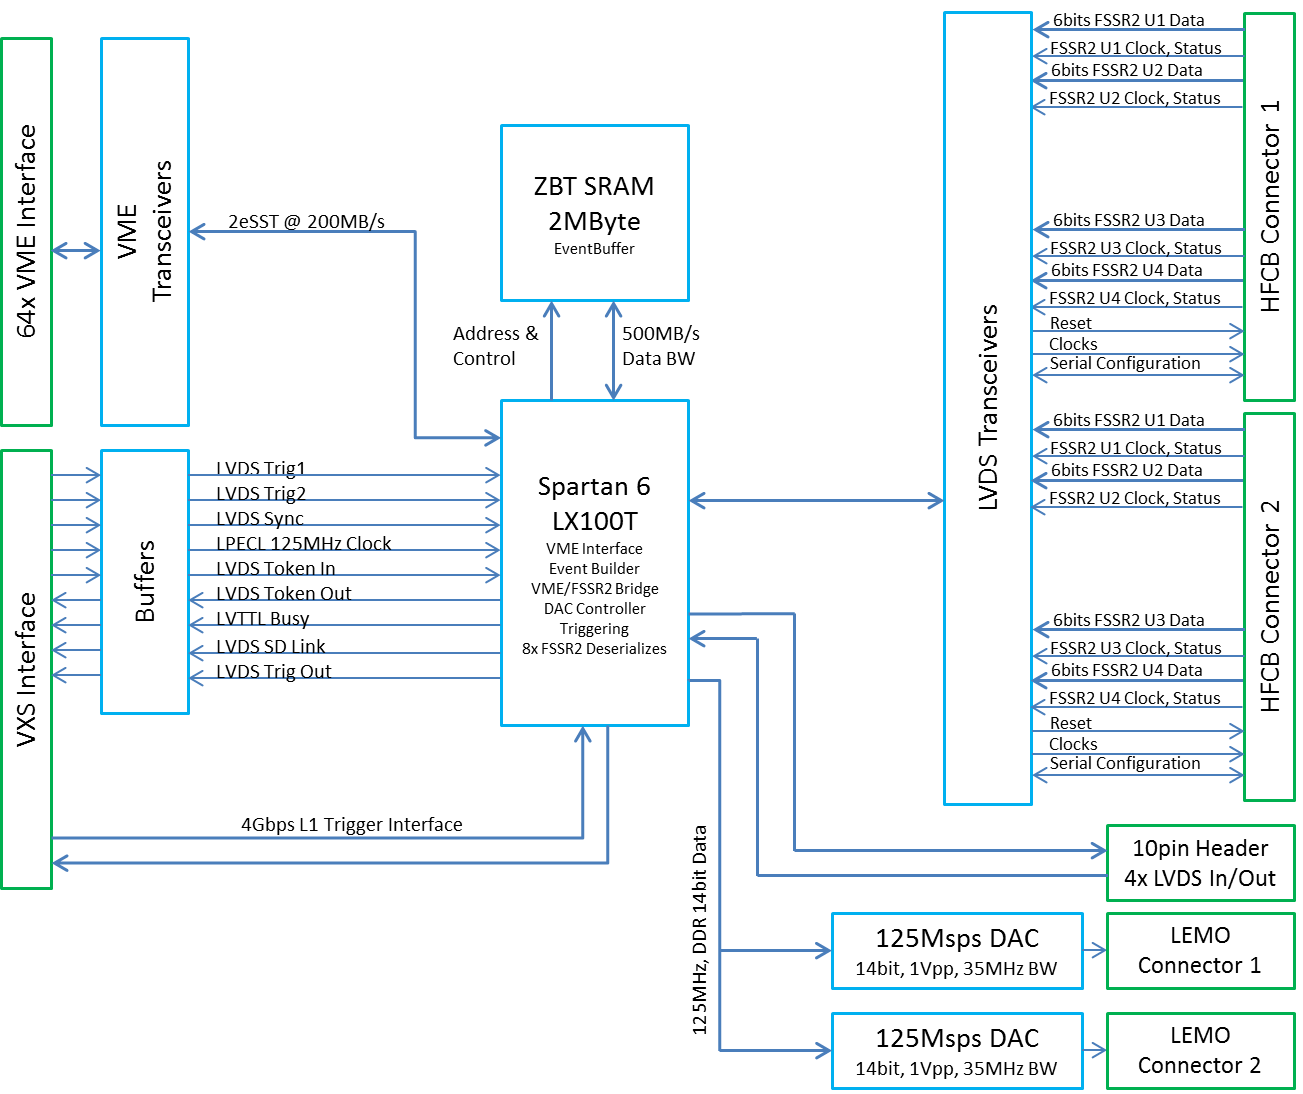
\includegraphics[width=1.0\columnwidth,keepaspectratio]{img/vscm_blockdiagram.png}
	\caption{VSCM Hardware Diagram}
	\label{fig:vscm_blockdiagram}
\end{figure}


\subsection{SSP Board as ffber Readout Module}

The SubSystem Processor (SSP \cite{ssp-ref}) was originally designed to work as part of CLAS12 Trigger System. It is used to readout some front-end electronics in the DAQ system as well. The board description can be found in the CLAS12 Trigger System article \cite{trig-ref}.
\section{Calibration}

Since the SVT modules are designed with a binary readout system, the analog channel response cannot be measured directly. Instead, the analog response is reconstructed by injecting a calibration charge on the channel and measuring the corresponding occupancy over a range of threshold values. 

\begin{figure}[hbt] 
	\centering 
	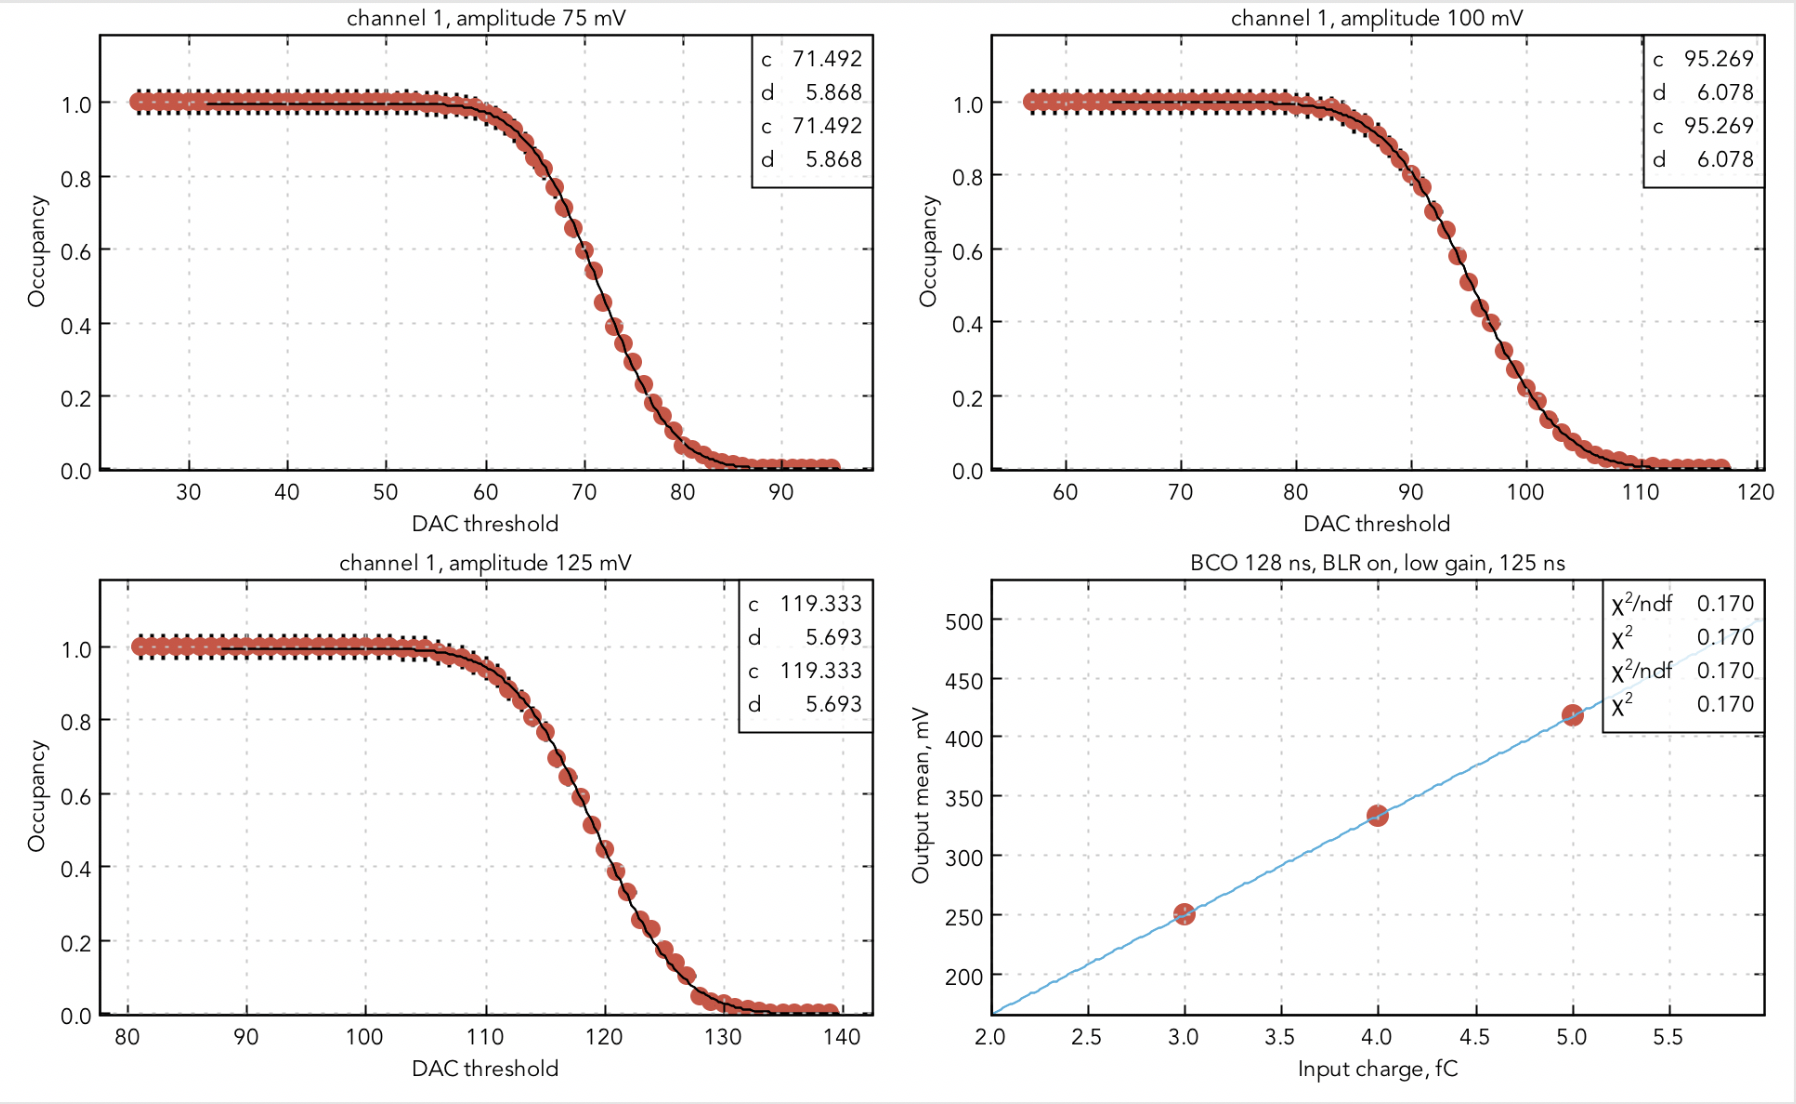
\includegraphics[width=1.0\columnwidth,keepaspectratio]{threshold-scan.png}
	\caption{Threshold scan on a single representative SVT channel.}
	\label{fig:threshold-scan}
\end{figure}

The output signals from the FSSR2 chip can be converted to charge using either internal or external calibration pulses. Because external pulser can be set to higher frequency than internal pulser without affecting the calibration process, external pulser circuit was added to the HBCB and the VSCM. Noise is measured using external, low frequency calibration charge injected in the absence of signal. The injected charge is shaped and amplified in the analog circuitry to form an output signal. The discriminator threshold determines whether or not the output signal corresponded to a hit. The probability that the injected charge produces a hit depends on the setting of the discriminator threshold. The average hit probability is measured by repeating the process of injecting charges and counting the fraction of readout triggers that produced a hit. This measurement is repeated over a range of threshold settings to produce an occupancy plot. 

The occupancy plots are measured setting the pulser amplitude at fixed values and changing the comparator thresholds. Each point of an occupancy plot represents the percentage of times that the comparator fires for a certain value of injected charge. In Fig.~\ref{fig:threshold-scan} presented three occupancy plots taken at different pulser amplitudes and the response plot showing the linear dependence of the output pulse height on the input charge in the operation region of the preamplifier. In between the high and low threshold regions, the occupancy curve is described by an error function, or S-curve, which can be fitted to the occupancy histogram for each channel, producing a mean value (discriminator threshold) and standard deviation (noise). The conversion from mV to electrons is performed considering a nominal value for the FSSR2 injection capacitance of 40~fF. 

\begin{figure}[hbt] 
	\centering 
	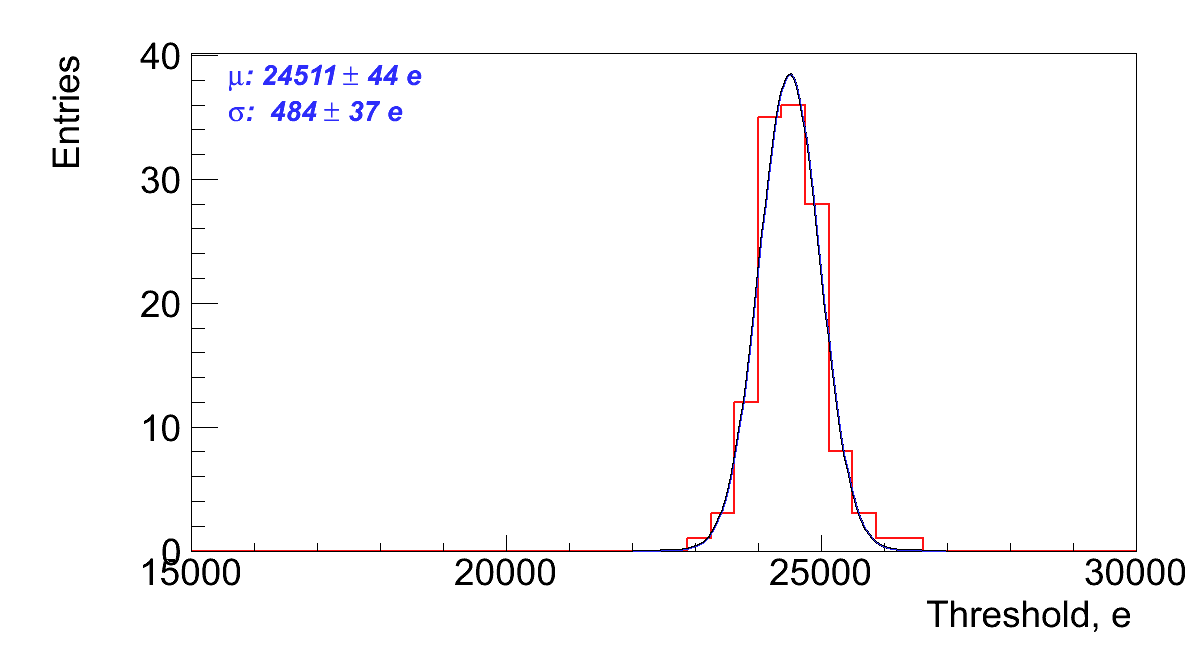
\includegraphics[width=0.8\columnwidth,keepaspectratio]{thrdisp.png}
	\caption{Typical threshold dispersion within a chip.}
	\label{fig:thrdisp}
\end{figure}

Threshold charge must be the same across the channels in a detector, otherwise the track-finding algorithms would be biased by the potential extra hits. Any spread in the response among the different channels of a chip results in a spread of the efficiency and noise occupancy which degrades effective performance. This leads to a requirement that the channel-to-channel variations in threshold and noise are kept to a minimum. Threshold dispersion is defined to be a standard deviation of the distribution of means obtained from the parameters of the complementary error function fit. The noise and threshold dispersion constants for each individual detector channel are measured and the values are used by the zero-suppression algorithms implemented in the core logic of the FSSR2 and by calibration procedures to identify defective channels. A comparison of the noise for 33~cm strips with the threshold spread demonstrates that the threshold spread is negligible compared to the noise and does not affect the efficiency and noise occupancy (see Fig.~\ref{fig:thrdisp}). The threshold dispersion agrees with expectations for the FSSR2 chip for the chosen settings.

SVT calibration data are stored in CLAS12 calibration database. The channel calibration table has columns corresponding to sector, layer, chip ID, mean, channel status (good, noisy, open, dead, or masked), ENC, gain, offset, V$_{t50}$ (threshold at 50$\%$ occupancy), and the threshold. There are 21504 rows in the channel calibration table. The ENC and gain are calculated using a calibration amplitude equal to 100 DAC.
The chip calibration table has columns corresponding to layer, sector, chip ID, ENC (electrons), gain (mV/fC), offset (mV), the threshold at 50$\%$ occupancy (V$_{t50}$, mV), threshold dispersion (electrons), chip gain (low, high), BLR mode (off, on), BCO time (ns), shaper time (ns), 8 ADC thresholds in DAC. There are 168 rows in the chip calibration table. 


\section{Event Reconstruction}

Reconstruction of the FT sub-detector information and the matching between the detectors to determine the type and
three-momentum of the incident particles is implemented in the CLAS12 Java reconstruction framework. Details on
the algorithms and implementation are provided in Ref.~\cite{reconstruction}. In the following we briefly summarize
the main steps and final outputs.

FT-Cal hits are reconstructed from the analysis of the recorded FADC information to extract energy and time;
hits are then associated based on position and time to form clusters whose energy and centroid position are used
as an initial seed to define the three-momentum of the incident particles. Similarly, FT-Hodo hits are reconstructed
from the FADC raw information and matched based on position and timing to form clusters of matching tiles in the
two layers of the detector. These are matched to clusters in the calorimeter based on position and time to distinguish
charged particles from neutrals. Finally, FT-Trk hits are also reconstructed from the raw data and geometrically
grouped to form clusters in each of the detector layers separately. Combinations of clusters in the $x-y$ layers of
each of the two sub-detectors are used to define crosses that are finally matched to calorimeter clusters to improve
the determination of the impact point of the particle.


\section{Simulation}

%\subsection{Expected physics performance}

%A series MC simulation have been used to calculate the acceptance of the central detector and have reconstructed physics parameters for types of events that are of interest. Fig. ... shows the missing mass resolution expected for MC simulation studies for a number of different reactions. For all cases studied, the results show that it is possible to identify the missing particle for each reaction.
%Figure ... shows the missing mass spectrum expected when pion is detected in the central tracker. There is sufficient resolution to study resonant production and to compare, for example, s, t, and u channel processes.

\subsection{Detector simulation}

A realistic model of the SVT has been developed, describing the location and composition of all modules, with material description based on the engineering drawings and assembly procedures, and confirmed by the survey measurements during integration. The SVT design and module layout were validated by Geant-4-based simulated detector performance studies demonstrating compliance with the technical requirements and engineering models. A 3D view of the simulated geometry of the SVT sensors is shown in Fig.~\ref{fig:svt3dview}. The SVT model is described in the simulation article of this volume. 

\begin{figure}[hbt] 
\centering 
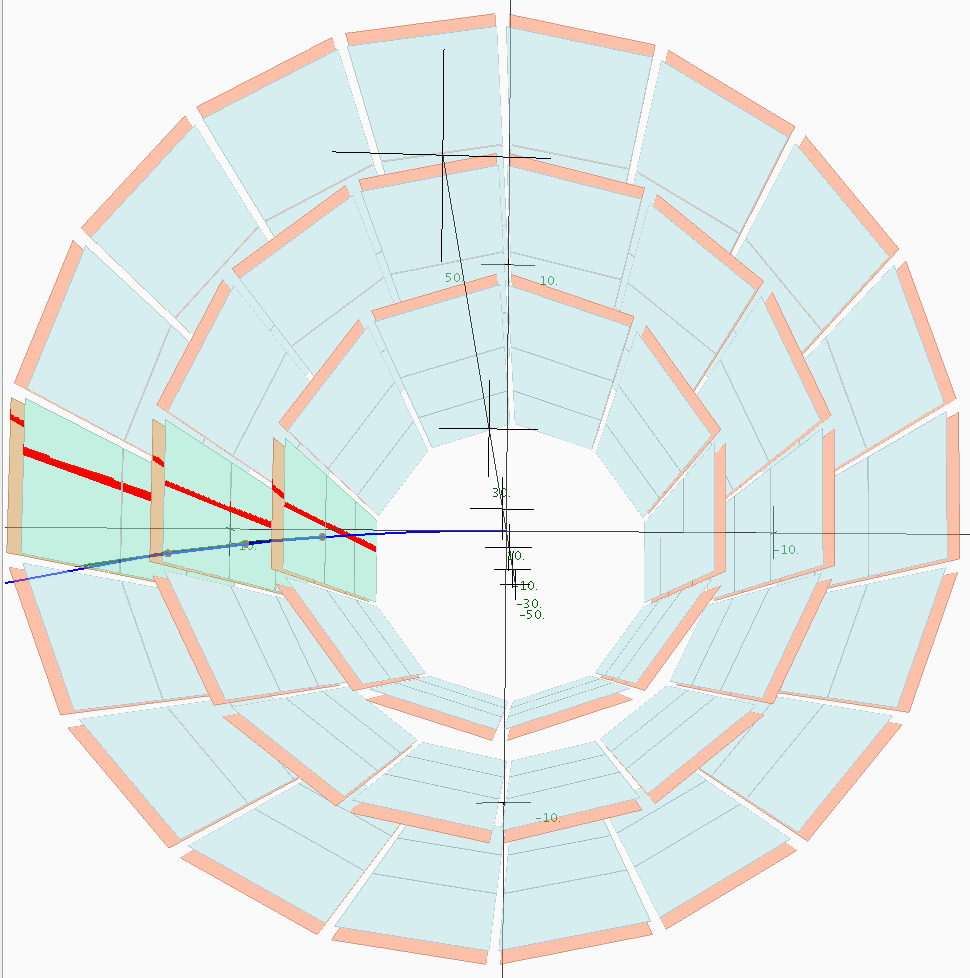
\includegraphics[width=1.0\columnwidth,keepaspectratio]{svt3dview.png}
\caption{3D view of the simulated SVT detector geometry.}
\label{fig:svt3dview}
\end{figure}

According to the results of GEANT simulation of the SVT, a resolution of 50~$\mu$m in the bending plane is needed to measure, with a precision better than 5$\%$, tracks with momentum up to 1~GeV (see Fig.~\ref{fig:PtRes}) \cite{MC1,MC2}. At low momenta the degradation of the resolution is caused by multiple scattering.

\begin{figure}[hbt]
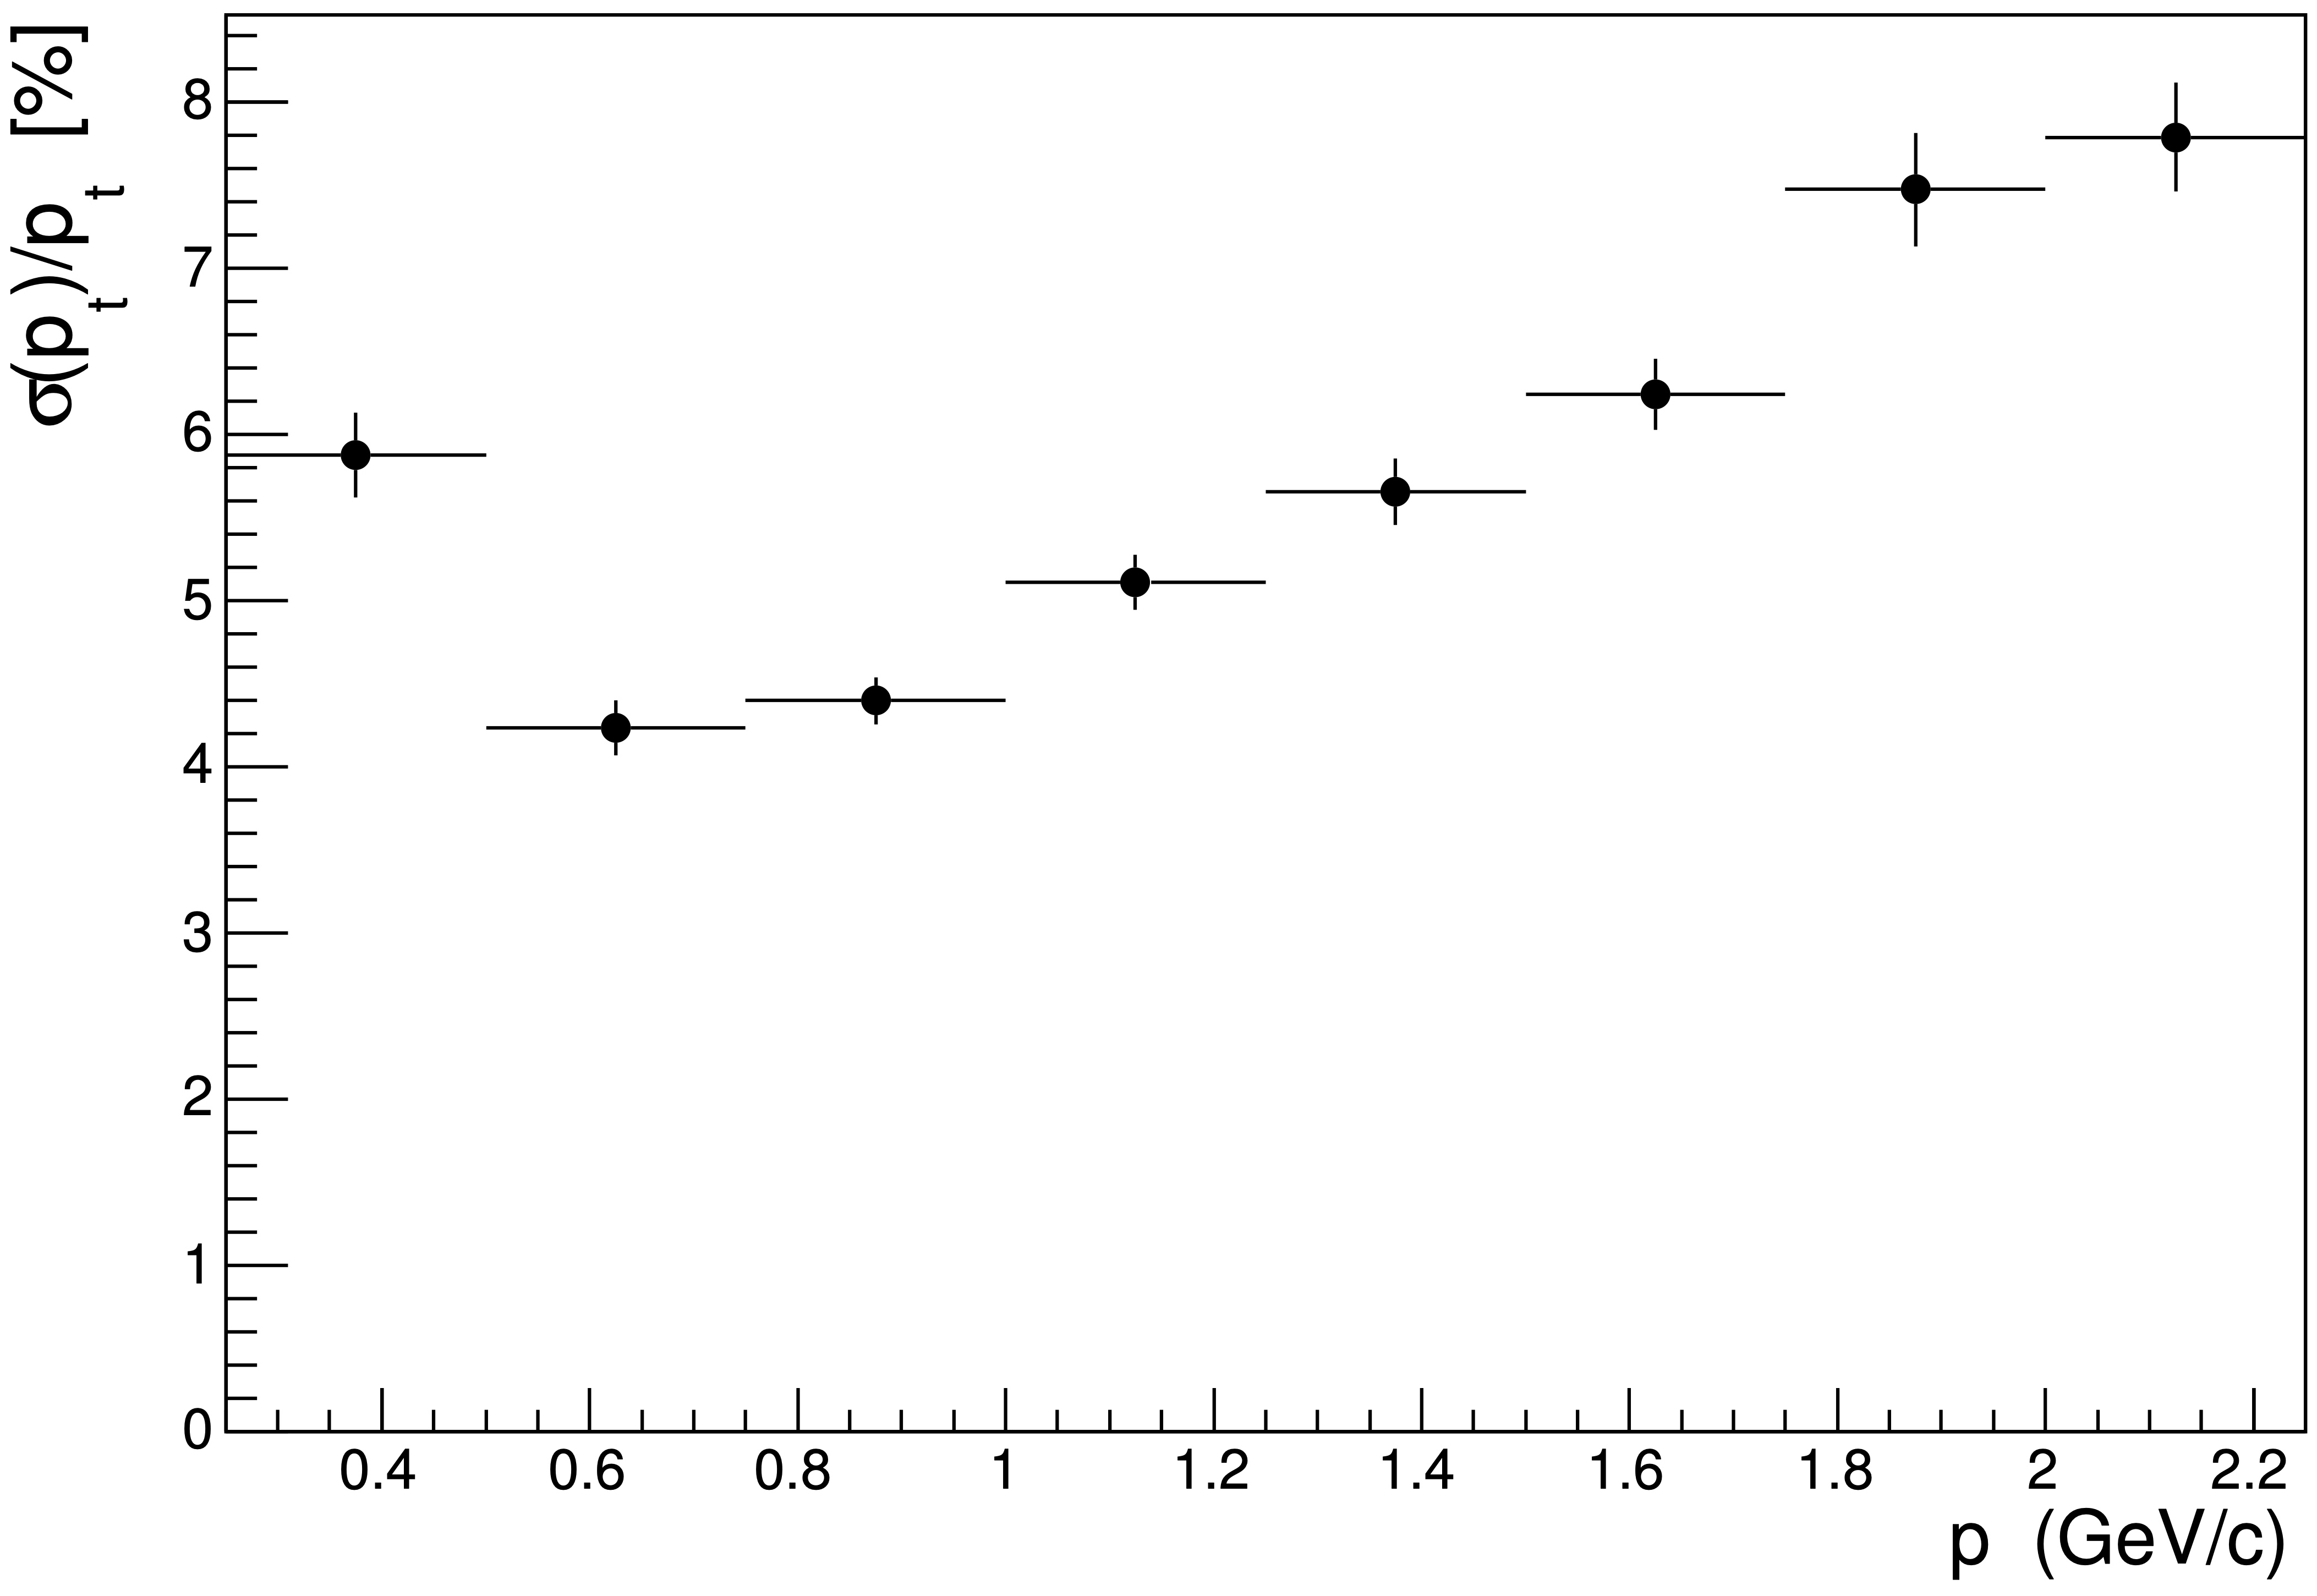
\includegraphics[width=1.0\columnwidth,keepaspectratio]{PtResol.jpg}
\caption{Simulated SVT momentum resolution.}
\label{fig:PtRes}
\end{figure}

Centroid residual distribution for the simulated muon tracks generated in the interval 0.5--2 GeV is shown in Fig.~\ref{fig:centroid-residual-mc}. Cluster centroids were calculated based on the charge weighting method. The spacial resolution of the sensors in the transverse plane using the ideal SVT geometry with no misalignments was found to be about 30~$\mu$m. 

\begin{figure}[hbt]
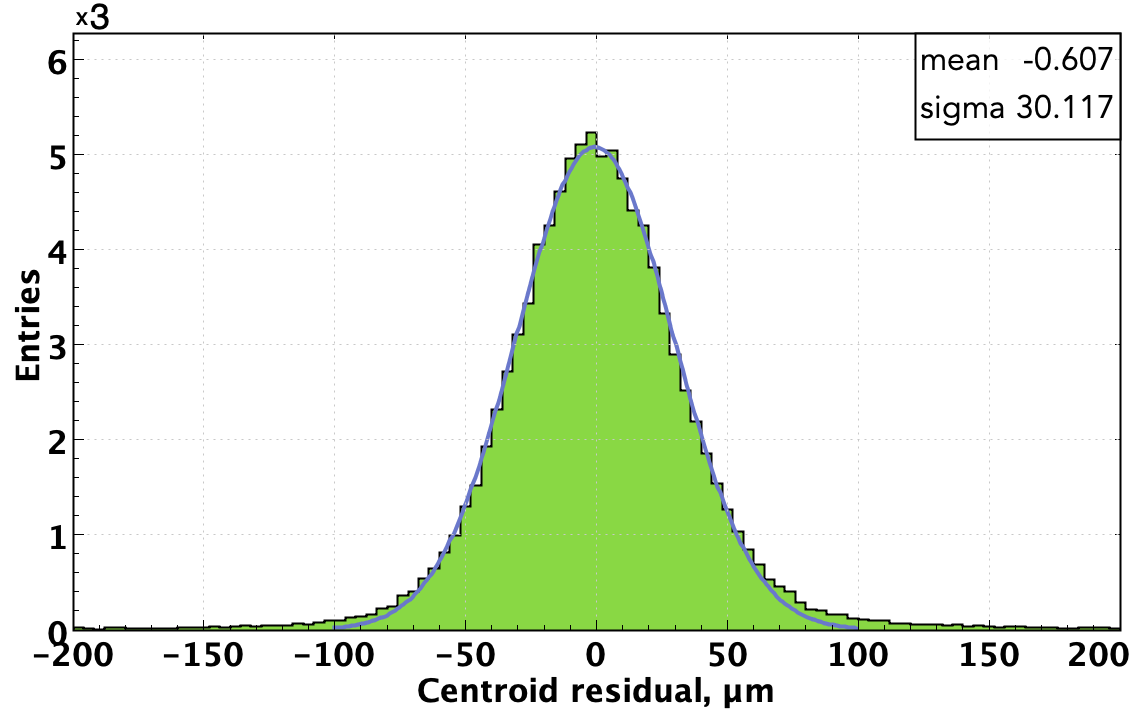
\includegraphics[width=1.0\columnwidth,keepaspectratio]{centroid-residual-mc.png}
\caption{Simulated centroid residual distribution for the SVT module.}
\label{fig:centroid-residual-mc}
\end{figure}

\subsection{Backgrounds, energy deposition, dose rates}

Radiation-induced bulk and surface detector damage studies have been conducted with charged hadrons, leptons, neutrons, and $\gamma$-ray photons. The radiation damage produced by different particles with different energies are scaled under the assumption of the Non-Ionizing Energy Loss (NIEL) hypothesis as the radiation damage in the silicon bulk depends only on the non-ionizing energy loss. The damage caused by different particles is referenced to the damage from 1 MeV neutrons. The standard value for the NIEL of 1 MeV neutrons is 95 MeVmb. 

\begin{figure}[hbt] 
\centering 
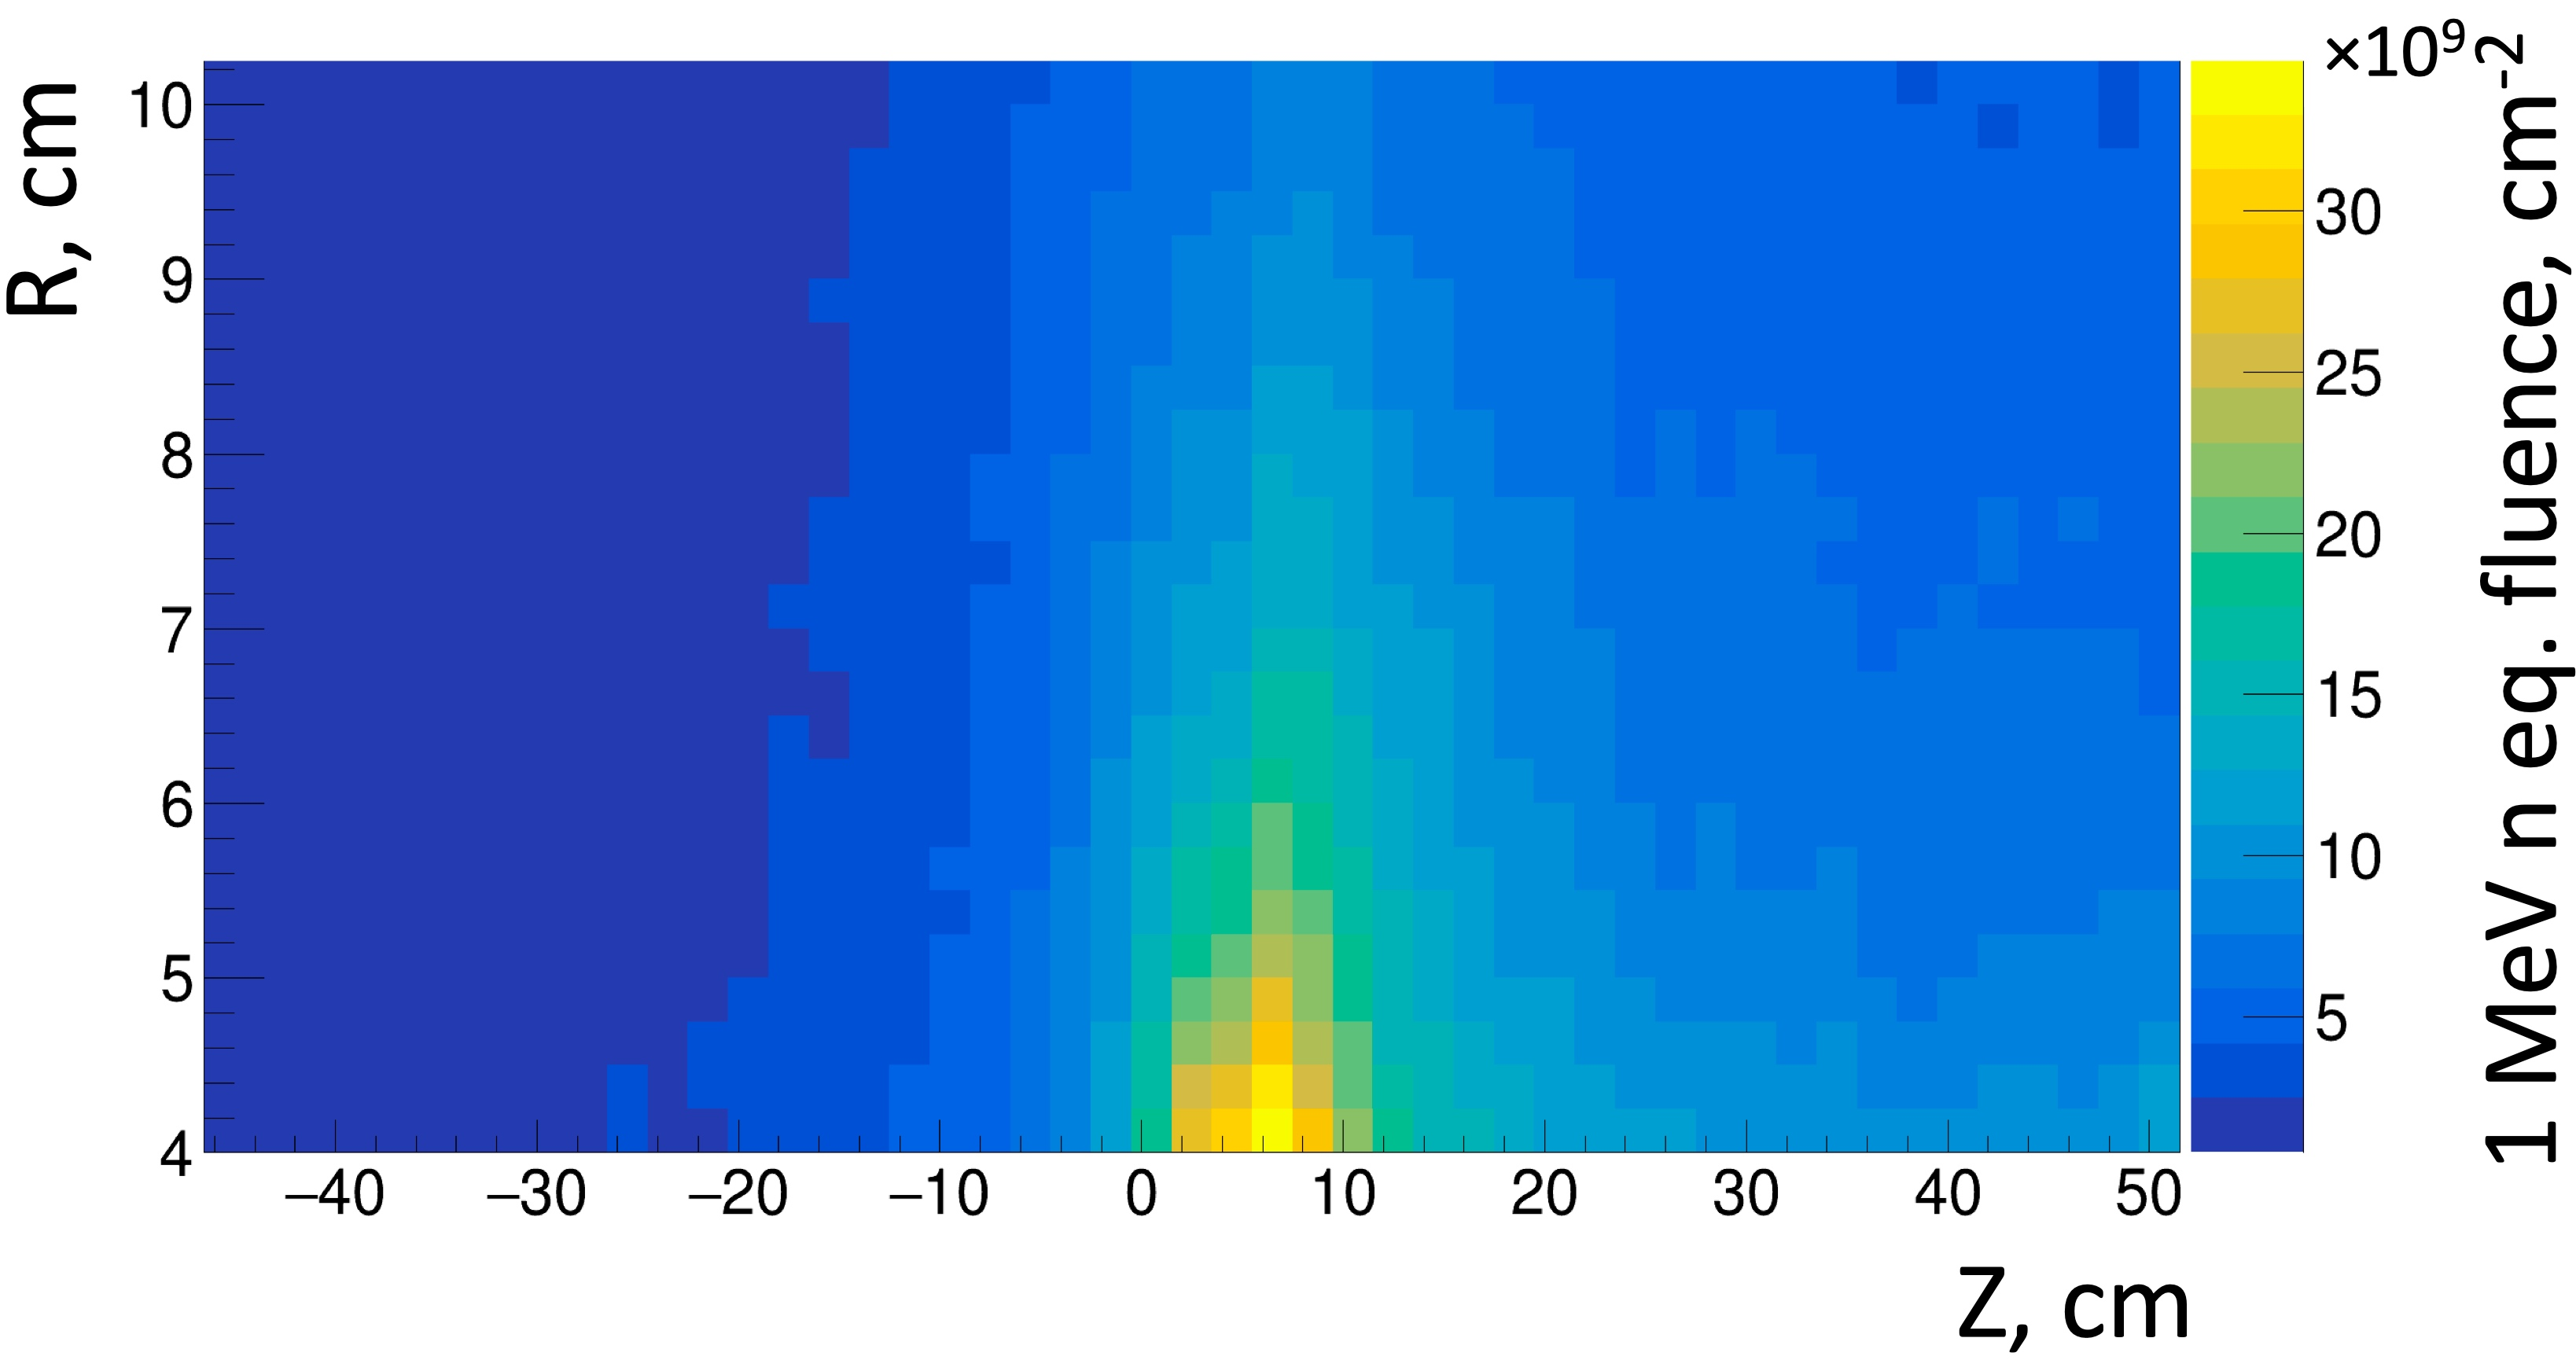
\includegraphics[width=1.0\columnwidth,keepaspectratio]{Pb_1MeVeq.jpg}
\caption{Accumulated 1MeV equivalent neutron fluence for the lead target.}
\label{fig:fluka1}
\end{figure}

To calculate the effects of different target configurations on the SVT detector,  FLUKA~\cite{FLUKA1, FLUKA2} simulations have been performed. In order to include the hadron electro-nuclear production, a dedicated source term has been used to enhance the physics production from the target, since it is a key in radiation estimates for targets with radiation length below 4$\%$. To assess the radiation damage to the SVT, the accumulated 1MeV neutron equivalent fluence has been recorded corresponding to the planned run conditions. For the experiment with lead target, the expected exposure was 240 h at beam current of 38 nA with electron beam energy of 6.6 GeV (Fig.~\ref{fig:fluka1}). For deuterium target, the study has been done for the accumulated charge of 108 mC at 11 GeV (Fig.~\ref{fig:fluka2}). In both scenarios the expected doses should not cause substantial degradation of the silicon sensors.

\begin{figure}[hbt] 
\centering 
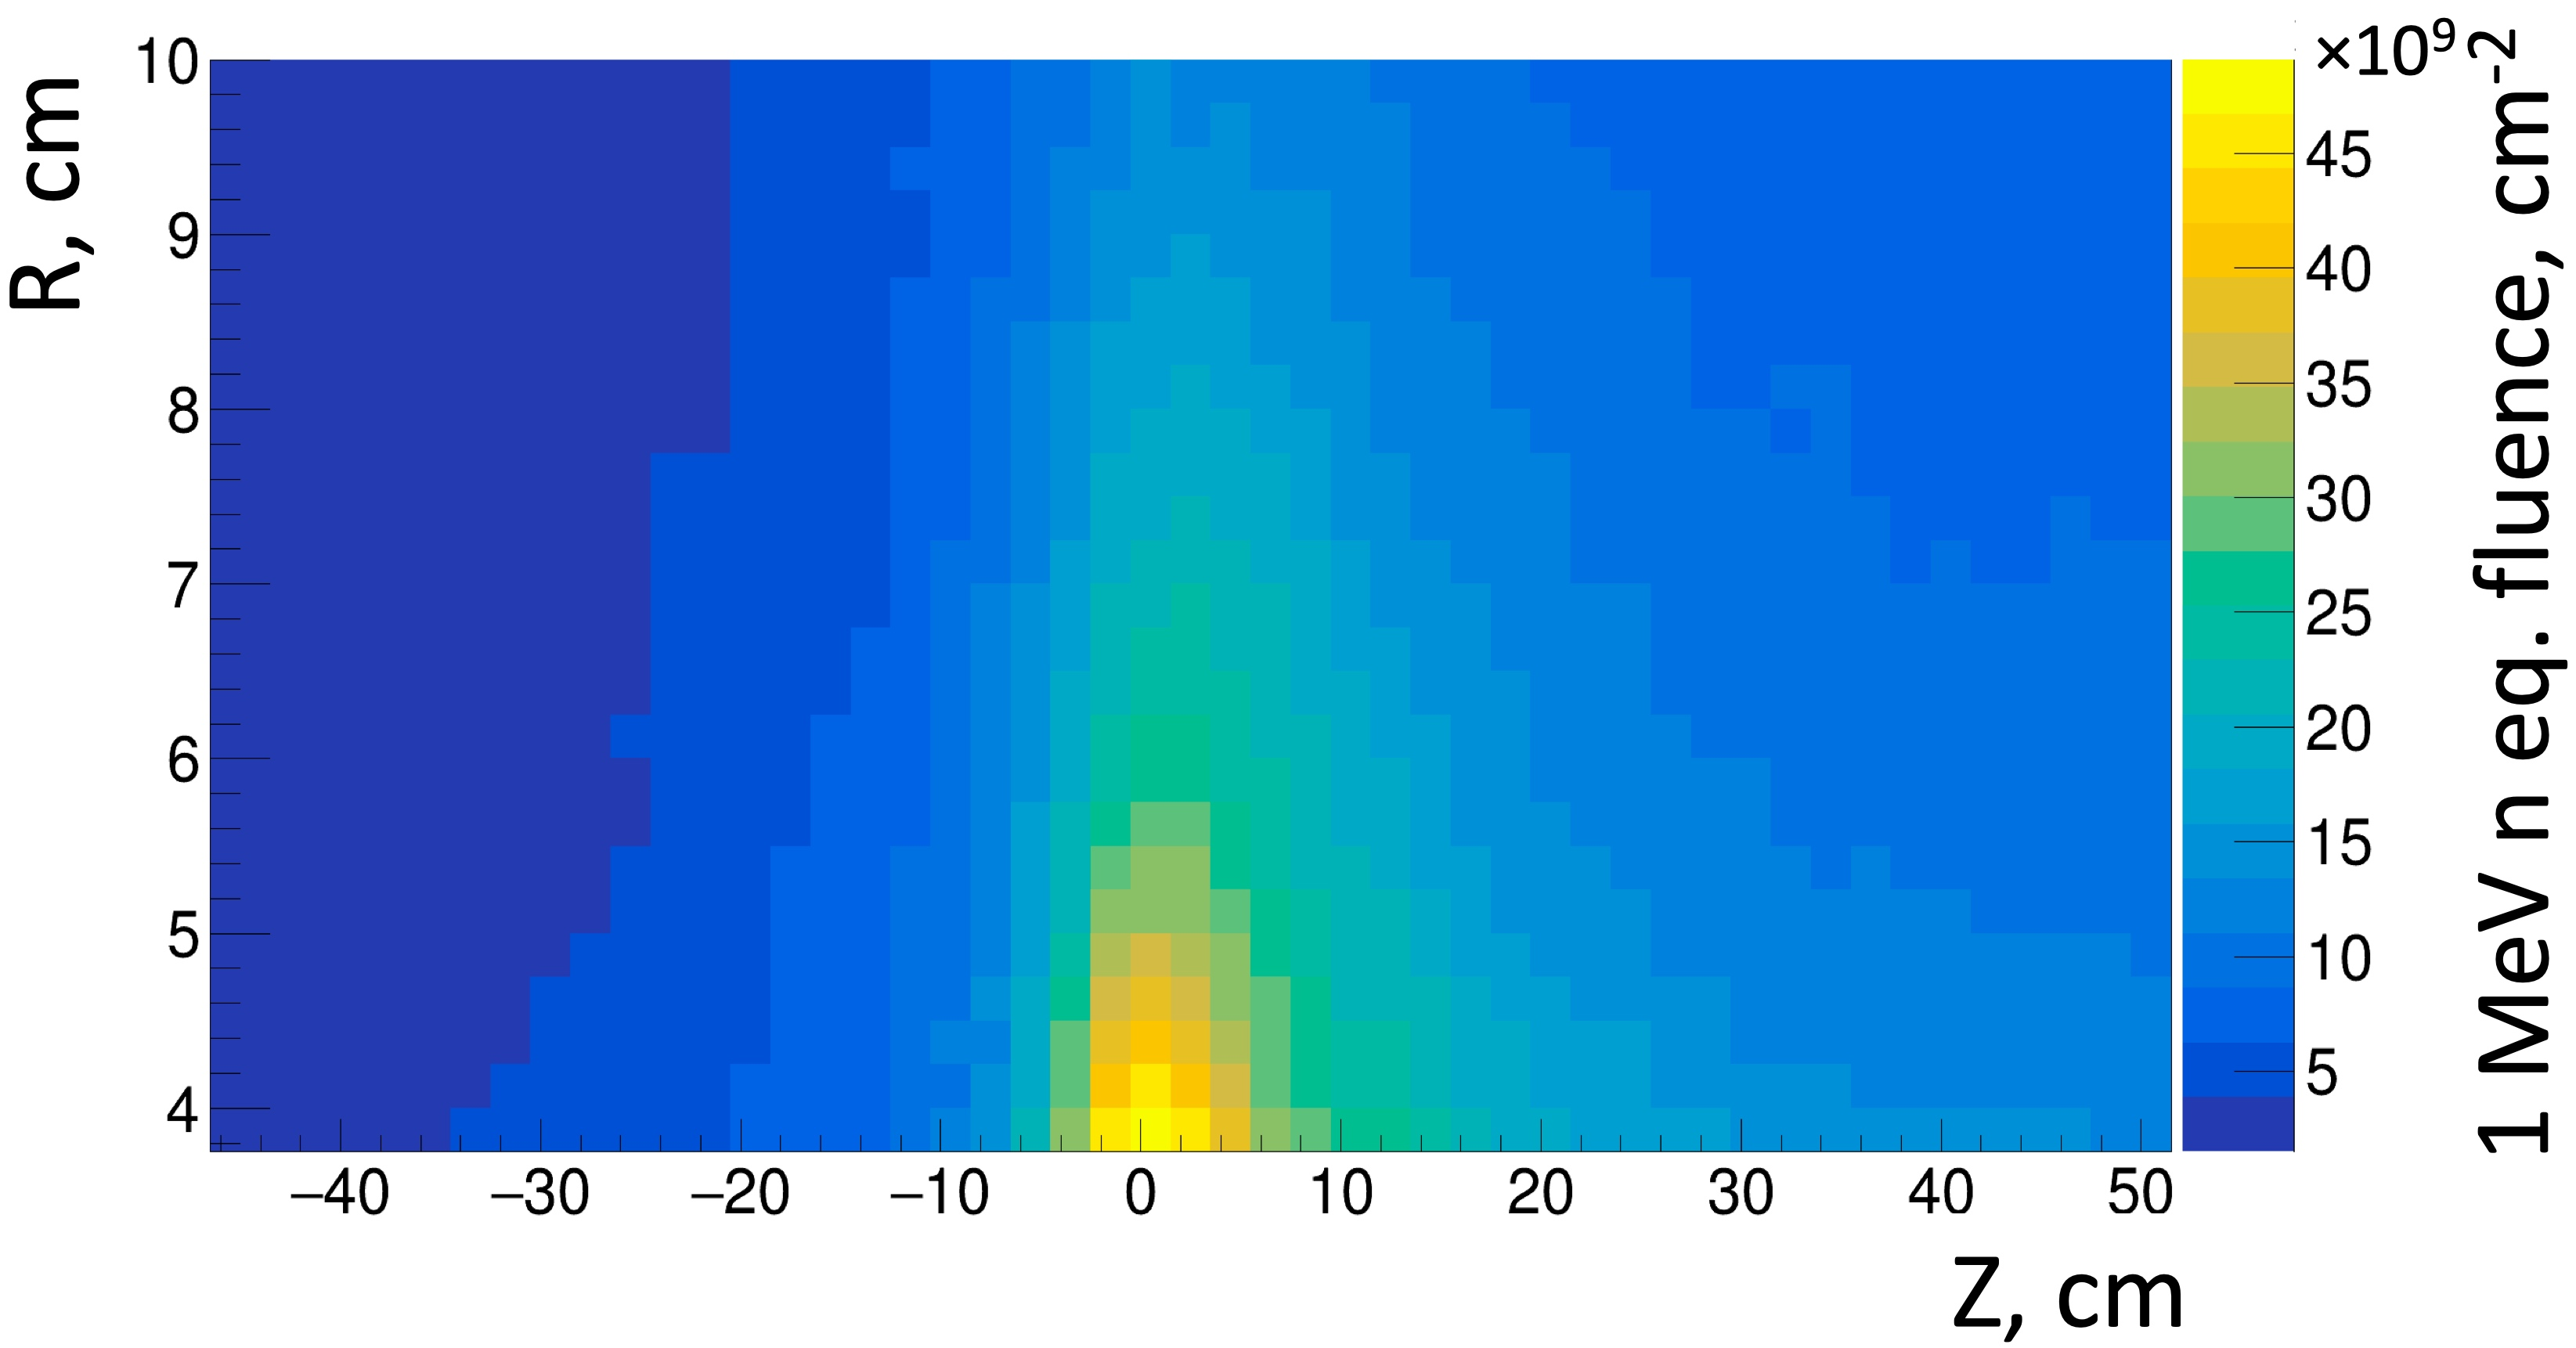
\includegraphics[width=1.0\columnwidth,keepaspectratio]{Deuterium_1MeVeq.jpg}
\caption{Accumulated 1MeV equivalent neutron fluence for the deuterium target.}
\label{fig:fluka2}
\end{figure}

FLUKA simulations of radiation damage levels have been performed in terms of 1MeV equivalent neutron fluence and high energy hadron equivalent fluence which is proportional to the rate of Single Event Effects (SEE)~\cite{FLUKA3}. Estimated levels of radiation damage in radial direction are presented in Fig.~\ref{fig:rad-levels-radial}) for liquid hydrogen and carbon targets at nominal beam currents. Also shown the radiation levels for the tagger magnet yoke during the beam tuning (see the beam line section in this volume).

\begin{figure}[hbt] 
\centering 
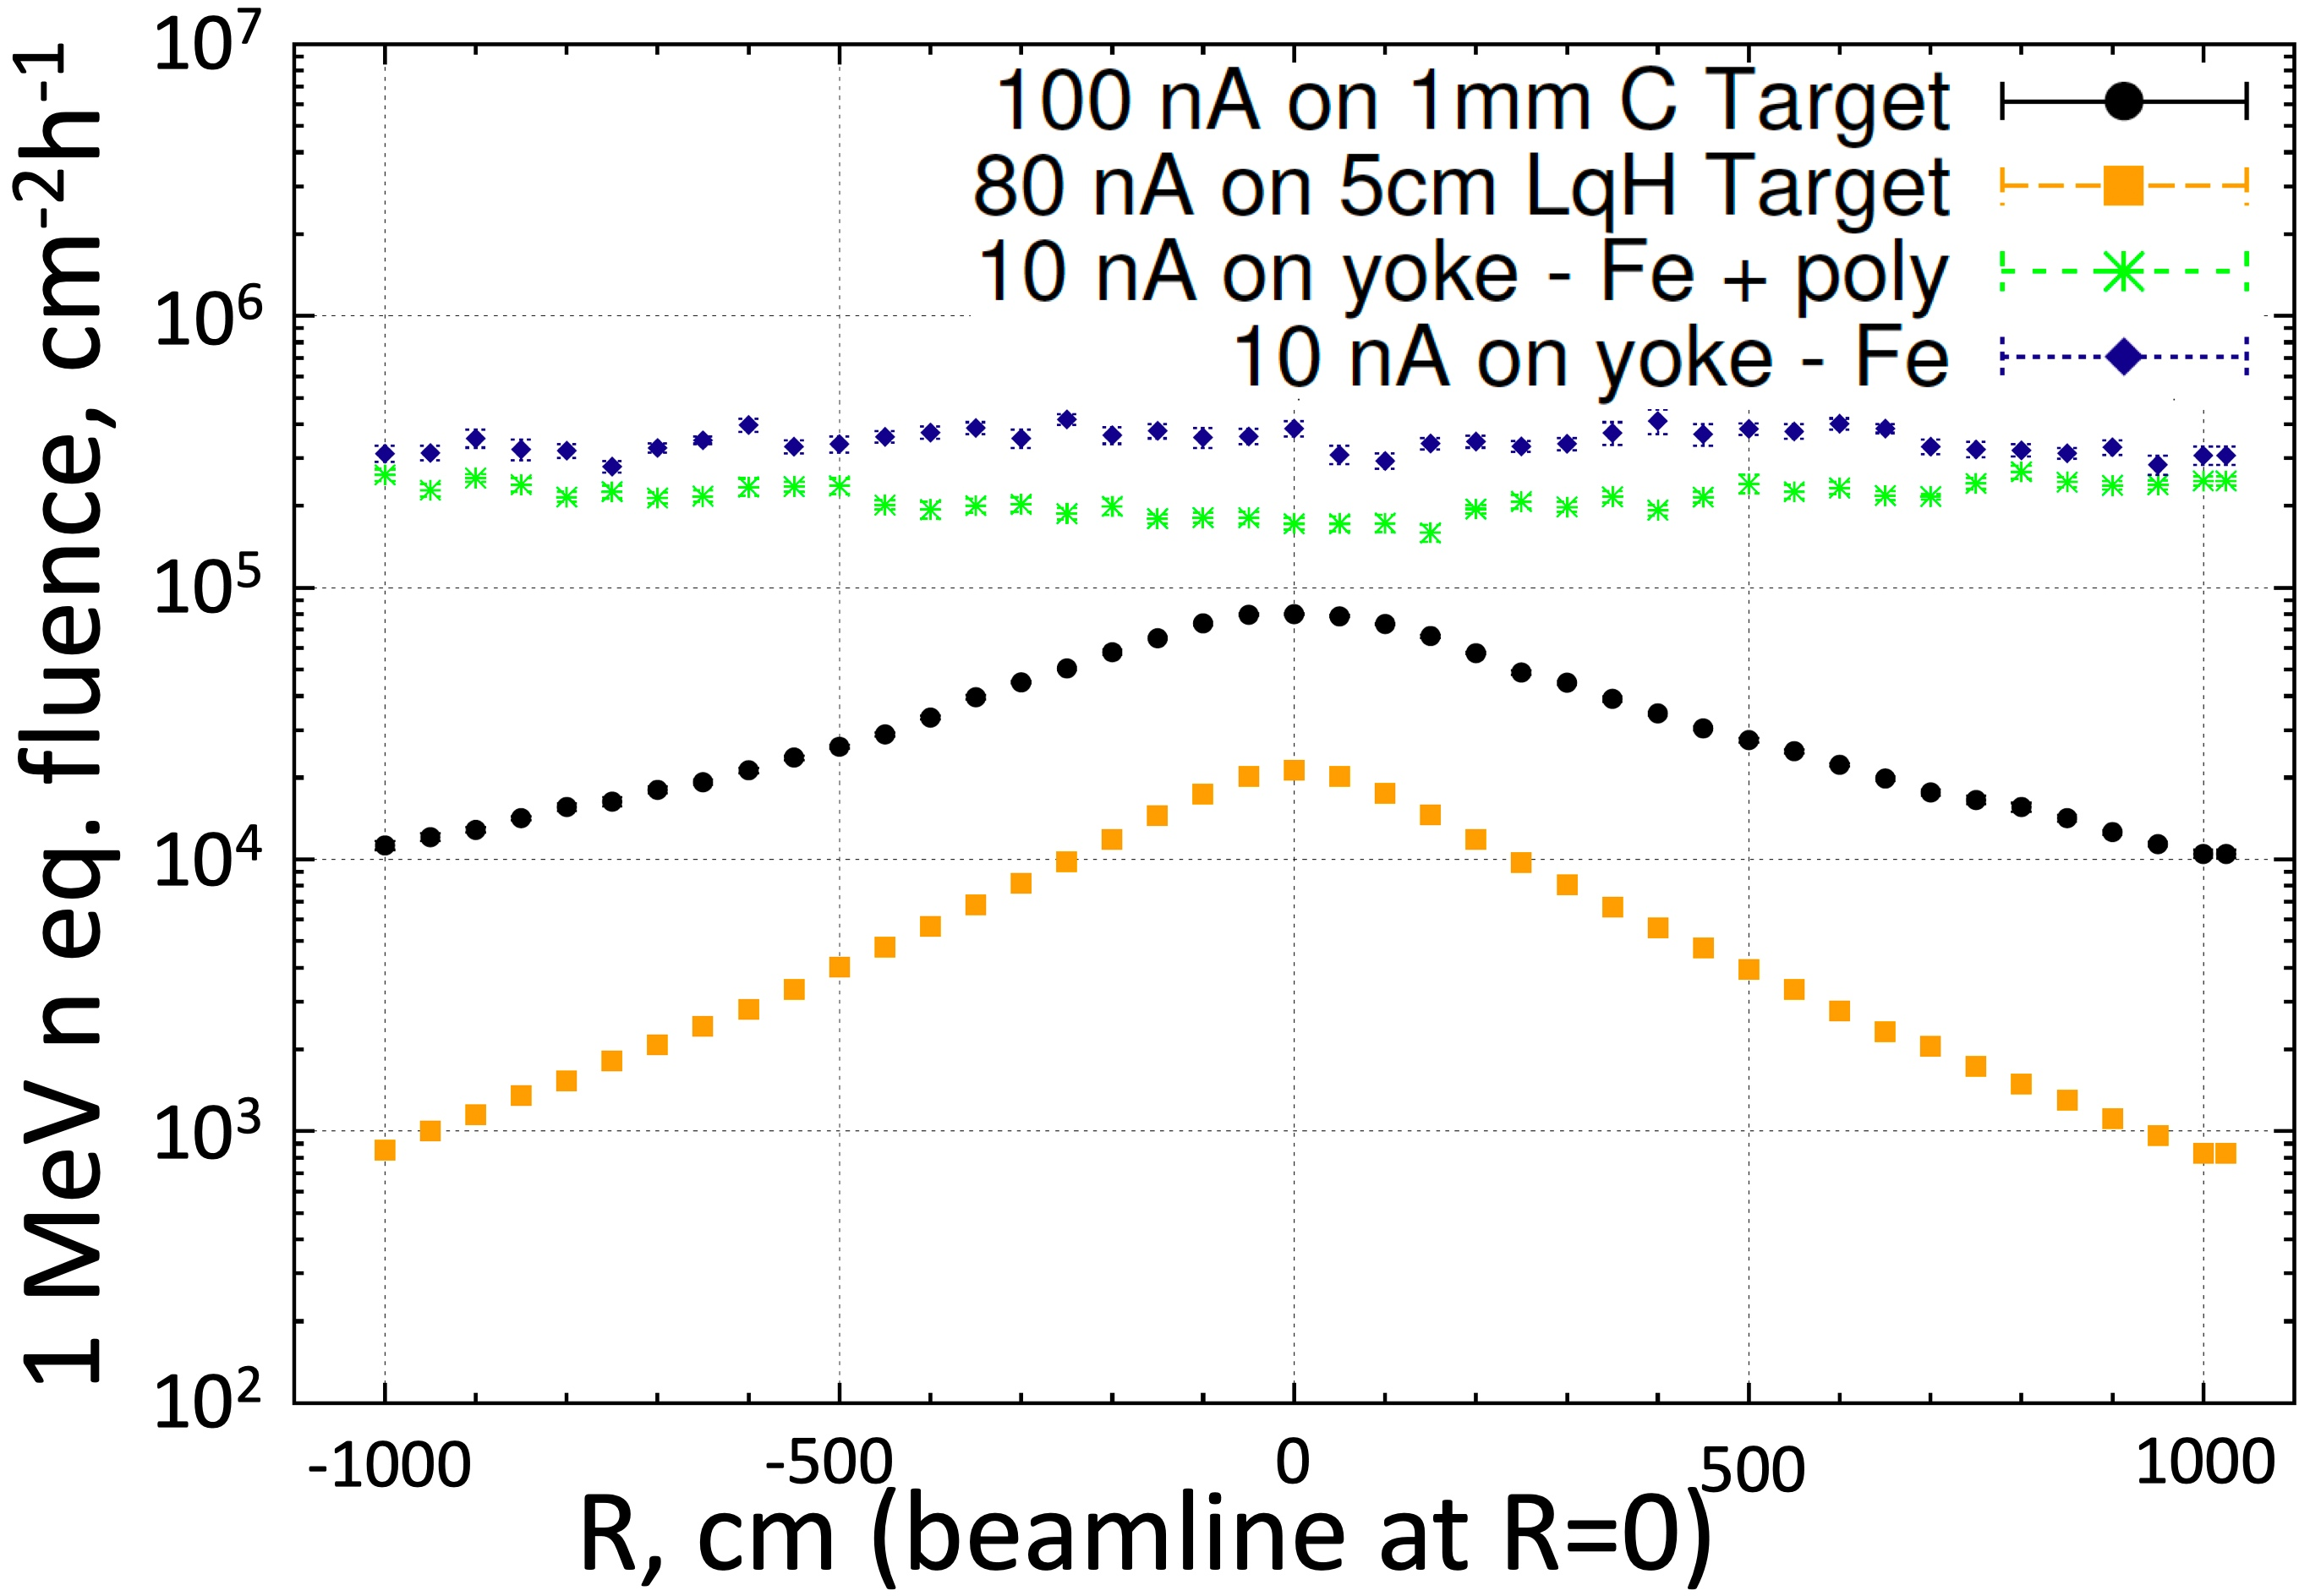
\includegraphics[width=1.0\columnwidth,keepaspectratio]{rad-levels-radial.jpg}
\caption{Estimated levels of radiation damage in radial direction in terms of 1MeV neutron equivalent fluence in silicon.}
\label{fig:rad-levels-radial}
\end{figure}

Simulations of beam-related backgrounds were performed for several thicknesses of a tungsten shielding cylinder around the CLAS12 target covering the first SVT layer. 
 
\begin{figure}[hbt] 
\centering 
\includegraphics[width=1.0\columnwidth,keepaspectratio]{rates-lh2.jpg}
\caption{Rates in the first SVT layer for a 5-cm long liquid hydrogen target at the nominal CLAS12 operating luminosity of 10$^{35}$cm$^{-2}$s$^{-1}$.}
\label{fig:rates-lh2}
\end{figure}

Fluences, radiation doses, and 1 MeV neutron damage rates in the SVT were calculated for different particles. Rates were estimated for liquid hydrogen, liquid deuterium, carbon, iron, and lead targets. For each event, 124,000 electrons going through the target within a 248.5-ns time window were simulated. This corresponds to the full CLAS12' 10$^{35}$cm$^{-2}$s$^{-1}$ luminosity on a 5-cm-long liquid-hydrogen target at 11 GeV beam energy. Rates in the first SVT layer for a liquid-hydrogen target are shown in Fig.~\ref{fig:rates-lh2}. For carbon target at a threshold of 40 keV the hadronic rate was estimated to be 5 MHz (total rate 40 MHz) with strip hit rates of 3.1 kHz (region 1), 2.2 kHz (region 2), and 1.7 kHz (region 3). The energy deposited in layer 1 for the electromagnetic and the hadronic particles is shown in Fig.~\ref{fig:energy-deposited-l1}. At a threshold of 30 keV, 92$\%$ of the electromagnetic background is rejected while preserving  99.5$\%$ of the signals coming from the hadrons~\cite{TDRSVT}.

\begin{figure}[hbt] 
\centering 
\includegraphics[width=1.0\columnwidth,keepaspectratio]{energy-deposited-l1.png}
\caption{Energy deposited in the SVT layer 1 for electromagnetic and hadronic particles for a liquid hydrogen target at the nominal CLAS12 operating luminosity.}
\label{fig:energy-deposited-l1}
\end{figure}

A tungsten shield 51~$\mu$m thick is installed on the target scattering chamber. The shield consists of 2 sheets mounted over the top and bottom halves of the foam cylinder referenced to the SVT common ground. The SVT rates and radiation damage benefit from the inclusion of the tungsten shield. The rates have been compared with physics run data at several beam currents.

While the gamma fluences / doses show a dramatic decrease with the introduction of shielding, the total fluences and doses decrease significantly for the thinner configuration and do not vary much for thicker tungsten (see Fig.~\ref{fig:rates-l1}). The photon radiation dose becomes negligible for 50 $\mu$m or more of tungsten with total 1 MeV equivalent radiation dose about 65 krad per year on a liquid-hydrogen target. For 15 years of running the experiment on a carbon target the estimated radiation dose for the sensors is 2.5~Mrad (with 50 $\%$ operation) \cite{TDRSVT}. 

\begin{figure}[hbt] 
\centering 
\includegraphics[width=1.0\columnwidth,keepaspectratio]{rates-l1.jpg}
\caption{Rates in the first SVT layer for different tungsten shield thickness from 50 to 500 $\mu$m for a liquid hydrogen target at the nominal CLAS12 operating luminosity. No energy threshold cut applied.}
\label{fig:rates-l1}
\end{figure}

An estimate of the double hit rate was performed. Fig.~\ref{fig:double-hit-rate} shows the probability of the double hits in the inner region of the SVT. The ratio of the double hits to the single hits was found to be about 1$\%$.

\begin{figure}[hbt] 
\centering 
\includegraphics[width=1.0\columnwidth,keepaspectratio]{double-hit-rate.jpg}
\caption{Double hit fraction in the region 1 with liquid hydrogen target.}
\label{fig:double-hit-rate}
\end{figure}

\subsection{Magnetic Field}

Due to the constrains on the maximum length of the cables, the readout, slow controls, and power supply crates are installed on a movable service cart within few meters from the detector. To assess the potential impact of the solenoid field on the SVT DAQ, a magnetic field map was simulated for the location of the power supply and readout crates. Fig.~\ref{fig:solenoid-field}) shows that the maximum strength of the field for the crates is at an acceptable level of 100 G.

\begin{figure}[hbt] 
\centering 
\includegraphics[width=1.0\columnwidth,keepaspectratio]{solenoid-field.jpg}
\caption{Solenoid field map at the location of the SVT service cart.}
\label{fig:solenoid-field}
\end{figure}




\section{Performance}The HTCC is one of the major CLAS12 systems used in experiments with the electron beam. The most important aspects of the HTCC performance are that it provides good timing, high electron detection efficiency, high signal strength, and high rejection factor of charged pions. All these parameters are critical for the quality of the data obtained in experiments since the detector, in combination with the forward calorimeter [ref. to ECAL], provides a fast trigger signal for CLAS12. As shown in section 6 the MC prediction for the HTCC for electrons is $\approx$100\%. Fig.~\ref{fig:RAFO_2GeV}. shows the experimentally measured electron detection efficiency for elastically scattered electrons at 2 GeV. The corresponding thresholds applied were approximately 2.5 photoelectrons. Measurements were performed using a special procedure with a random trigger that was not correlated with the HTCC. There were observed 27 events not detected by the HTCC due to the applied threshold. As shown, the electron detection efficiency is $\eta$ = (99$\pm$0.2)\%, which is in good agreement with the MC estimate. This result can be considered as a conservative estimate due to relatively high threshold used in measurements. Moreover, electrons travel a longer distance in the radiator gas (10 \% to 30 \% difference depending on a scattering angle). For these electrons the signal strength is higher, and therefore the detection efficiency is higher also as compared with the aforementioned efficiency for the elastically scattered electrons.   

\begin{figure}[!ht]
    \centering
    \includegraphics[width=1.0\linewidth,trim={0.0cm 0.0cm 0.0cm 0.0cm},clip]{images/RAFO_2GeV.jpg}
    \caption{Electron detection efficiency for elastically scattered electrons at 2 GeV. Data are obtained with the random trigger not correlated with the HTCC or other detector components of CLAS12.}
    \label{fig:RAFO_2GeV}
\end{figure}

Fig.~\ref{fig:positivePNPEC6595} shows the response of the detector in a wide range of particle momentum. The increase of number of events at high momenta is due to registration of charged pions (above threshold of their registration in the HTCC) and this is clearly illustrated.

\begin{figure}[!ht]
    \centering
    \includegraphics[width=1.0\linewidth,trim={0.0cm 0.0cm 0.0cm 0.0cm},clip]{images/positivePNPEC6595.png}
    \caption{Distributions of the HTCC response in a wide momentum range, including the region beyond the threshold of charged pion registration. Data obtained for positrons and $\pi^{+}$-mesons.}
    \label{fig:positivePNPEC6595}
\end{figure}

\begin{comment}
As shown bellow in the Fig.~\ref{fig:avgNPE_Theta_Phi_Dev_Build-2_NO_HOLES} the signal strength goes up for the utmost mirrors (large electron scattering angles). This is because electrons travel a longer distance in the radiator gas (10\% to 30\% difference depending on angle.) In other words the electron detection efficiency obtained for elastically scattered electrons at 2 GeV can be considered as as a conservative estimate for the efficiency of electron detection at larger angles.
\end{comment} 

The signal strength in the HTCC depends on the actual properties of the mirror facets, such as their final shape and reflectance. The accuracy of the combined mirror assembly and the alignment of the HTCC components (mirror, PMTs, Winston Cones), and the composition of the radiator gas all influence the final results. The FADC histogram of  the typical signal strength distribution obtained in one half-sector \#1 and \#2 of Sector 1 is shown in Fig.~\ref{fig:Signal_S1_HS1_HS2_R1_R2}. The signal strength for scattered electrons averaged over all HTCC channels is shown in Fig.~\ref{fig:Average_HTCC_Signal}. The experimentally measured mean value of 16.3 phe is close to Monte-Carlo simulation results, (see Fig.~\ref{fig:10cm_Targ_5T_Field_Phi}).

\begin{figure}[!ht]
    \centering
    \includegraphics[width=1.0\linewidth,trim={0.0cm 0.0cm 0.0cm 0.0cm},clip]{images/Signal_S1_HS1_HS2_R1_R2.jpg}
    \caption{Typical distributions of the signal strength in channels covering polar angles in the range of $5^\circ$ to $12.5^\circ$ (Ring 1) and $12.5^\circ$ to $20.0^\circ$ (Ring 2) within azimuthal interval of $60^\circ$.}
    \label{fig:Signal_S1_HS1_HS2_R1_R2}
\end{figure}

\begin{figure}[!ht]
    \centering
    \includegraphics[width=1.0\linewidth,trim={0.0cm 0.0cm 0.0cm 0.0cm},clip]{images/Average_HTCC_Signal.jpg}
    \caption{The HTCC average signal strength for electrons from beam data.}
    \label{fig:Average_HTCC_Signal}
\end{figure}

Fig.~\ref{fig:HTCC_Response_run4013} shows the HTCC response for different electron momenta. Fig.~\ref{fig:avgNPE_Theta_Phi_Dev_Build-2_NO_HOLES}  shows the distribution of the HTCC response over the entire face of the mirror in the $x-y$-plane. Similar distribution is shown in Fig.~\ref{fig:avgNPE_XY_Dev_Build_02npe} obtained at the lower electron detection threshold of 0.2 photoelectrons. At the large electron scattering angles in range of 27.5$^\circ$ to 35$^\circ$, the statistics is lower. Fig.~\ref{fig:statistics_Theta_Phi_Dev_Build_NO_HOLES} shows the distribution of statistics in all 6 sectors. The data shows that the integrated signal strength is about 16.5 photoelectrons.

\begin{figure}[!ht]
    \centering
    \includegraphics[width=1.0\linewidth,trim={0.0cm 0.0cm 0.0cm 1.73cm},clip]{images/HTCC_Response_run4013.png}
    \caption{The HTCC response for electrons: signal strength vs. momentum at 10.6 GeV energy.}
    \label{fig:HTCC_Response_run4013}
\end{figure}

\begin{figure}[!ht]
    \centering
    \includegraphics[width=1.0\linewidth,trim={0.0cm 0.0cm 0.0cm 1.67cm},clip]{images/avgNPE_Theta_Phi_Dev_Build-2_NO_HOLES.png}
    \caption{The HTCC response (in $N_{phe}$) for electrons in $x-y$-plane of the mirror.}
    \label{fig:avgNPE_Theta_Phi_Dev_Build-2_NO_HOLES}
\end{figure}

\begin{figure}[!ht]
    \centering
    \includegraphics[width=1.0\linewidth,trim={0.0cm 0.0cm 0.0cm 1.67cm},clip]{images/avgNPE_XY_Dev_Build_02npe.png}
    \caption{The HTCC response (in $N_{phe}$) for electrons in $x-y$-plane of the mirror at the electron detection threshold of 0.2 photoelectrons.}
    \label{fig:avgNPE_XY_Dev_Build_02npe}
\end{figure}

\begin{figure}[!ht]
    \centering
    \includegraphics[width=1.0\linewidth,trim={0.0cm 0.0cm 0.0cm 1.67cm},clip]{images/statistics_Theta_Phi_Dev_Build_NO_HOLES.png}
    \caption{Distribution of statistics in all 6 sectors.}
    \label{fig:statistics_Theta_Phi_Dev_Build_NO_HOLES}
\end{figure}

We also note that in cases when the electrons cross the mirror close to its edges (at approximately at 5$^\circ$ and 35$^\circ$) one should expect unavoidable losses in the signal strength: some part of the Cherenkov light just passes by the mirror. As far as the internal borders between adjacent mirrors are concerned, there are similar losses that take place and are finally partially compensated due to the complete azimuthal symmetry of the detector, see Fig.~\ref{fig:avgNPE_Theta_Phi_Dev_Build-2_NO_HOLES}. The width of that area along internal boundaries that is deformed in the direction normal to the mirror face due to the shrinkage of the glue is estimated between $\sim$5 to $\sim$10 mm. This area includes the technological zone ~0.5 mm of width that is not reflecting the light at all. As a result these regions (width up to $\sim$10 mm) along internal boundaries between mirror facets defuse the light impinging the area, and therefore the signal strength is reduced. this edge effect is normal for the given design of the detector.


\section{Acknowledgements}

We appreciate the contribution of J.  Andresen, C. Britton, S. Chappa, A. Dyer, J. Hoff, V. Re, and T. Zimmerman to the design of the HFCB. We are grateful to administrative, engineering, and technical staff of Fermilab Silicon Detector Facility for excellent work on module assembly.

\section{Conclusions}

The SVT is installed in the CLAS experimental hall, performance of modules measured during detector integration has been confirmed. No channels were lost during the installation. SVT barrel has been electrically  tested with number of defective channels 0.1$\%$, well within the specification. The chip average ENC noise is uniform $\sim$1600 e in normal operating conditions. There is no evidence of coherent noise between the modules and other components. The tracker has been commissioned with cosmic rays and integrated as part of  CLAS central detector. Tracking performance was confirmed with beam data and matches physics requirements. 





\section{References}

\bibliography{bibfile}
\bibliographystyle{elsarticle-num}
\end{document}








